\documentclass[12pt,twoside]{report}

% some definitions for the title page
\newcommand{\reporttitle}{Nested Multiparty Session Programming in Go}
\newcommand{\reportauthor}{Benito Echarren Serrano}
\newcommand{\supervisor}{Prof. Nobuko Yoshida}
\newcommand{\secondmarker}{Dr. Iain Phillips}
\newcommand{\reporttype}{Final Report}
\newcommand{\degreetype}{MEng Computing} 

\newcommand{\comment}[1]{}
\newcommand{\white}{\ \ \ \ \ \ \ \ \ \ \ \ }
\newcommand{\pad}{\ \ \ \ \ \ }
% load some definitions and default packages
%%%%%%%%%%%%%%%%%%%%%%%%%%%%%%%%%%%%%%%%%
% University Assignment Title Page 
% LaTeX Template
% Version 1.0 (27/12/12)
%
% This template has been downloaded from:
% http://www.LaTeXTemplates.com
%
% Original author:
% WikiBooks (http://en.wikibooks.org/wiki/LaTeX/Title_Creation)
%
% License:
% CC BY-NC-SA 3.0 (http://creativecommons.org/licenses/by-nc-sa/3.0/)
% 
%
%%%%%%%%%%%%%%%%%%%%%%%%%%%%%%%%%%%%%%%%%
%----------------------------------------------------------------------------------------
%	PACKAGES AND OTHER DOCUMENT CONFIGURATIONS
%----------------------------------------------------------------------------------------
\usepackage[a4paper,hmargin=2.8cm,vmargin=2.0cm,includeheadfoot]{geometry}
\usepackage{textpos}
\usepackage[numbers]{natbib} % for bibliography
\usepackage{tabularx,longtable,multirow,subfigure,caption}%hangcaption
\usepackage{fncylab} %formatting of labels
\usepackage{fancyhdr} % page layout
\usepackage{url} % URLs
\usepackage[english]{babel}
\usepackage{amsmath}
\usepackage{graphicx}
\usepackage{dsfont}
\usepackage{epstopdf} % automatically replace .eps with .pdf in graphics
% \usepackage{backref} % needed for citations
\usepackage{array}
\usepackage{latexsym}
\usepackage{semantic}
\usepackage{xfrac}
\usepackage{fourier}
\usepackage{ amssymb }


\usepackage{listings}
\usepackage{color}


\lstset{frame=tb,
  language=Java,
  aboveskip=3mm,
  belowskip=3mm,
  showstringspaces=false,
  columns=flexible,
  basicstyle={\ttfamily},
  numbers=left,
  numberstyle=\tiny\color{gray},
  keywordstyle=\color{blue},
  commentstyle=\color{dkgreen},
  stringstyle=\color{mauve},
  breaklines=true,
  breakatwhitespace=true,
  tabsize=3,
  frame=single,
}
\definecolor{dkgreen}{rgb}{0,0.6,0}
\definecolor{gray}{rgb}{0.5,0.5,0.5}
\definecolor{mauve}{rgb}{0.58,0,0.82}
\definecolor{granate}{rgb}{0.68, 0.02, 0.55}

\lstdefinelanguage{Scribble}{
  keywords={global, protocol, rec, role, choice, at, continue, do, from, to, var, if, in, while, do, else, case, break, calls, new, nested, accept, invite, create},
  keywordstyle=\color{granate}\bfseries,
  ndkeywords={class, export, boolean, throw, implements, import, this},
  ndkeywordstyle=\color{darkgray}\bfseries,
  identifierstyle=\color{black},
  sensitive=false,
  comment=[l]{//},
  morecomment=[s]{/*}{*/},
  commentstyle=\color{dkgreen}\ttfamily,
  stringstyle=\color{dkgreen}\ttfamily,
  morestring=[b]',
  morestring=[b]"
}


% \usepackage[pdftex,pagebackref,hypertexnames=false,colorlinks]{hyperref} % provide links in pdf
\usepackage[pdftex,hypertexnames=false,colorlinks]{hyperref} % provide links in pdf

\hypersetup{pdftitle={},
  pdfsubject={}, 
  pdfauthor={},
  pdfkeywords={}, 
  pdfstartview=FitH,
  pdfpagemode={UseOutlines},% None, FullScreen, UseOutlines
  bookmarksnumbered=true, bookmarksopen=true, colorlinks,
    citecolor=black,%
    filecolor=black,%
    linkcolor=black,%
    urlcolor=black}

\usepackage[all]{hypcap}

% {} limita scope de color
% \newcommand{\global}{{\color{blue}\mathtt{global}}}

%\usepackage{color}
%\usepackage[tight,ugly]{units}
%\usepackage{float}
%\usepackage{tcolorbox}
%\usepackage[colorinlistoftodos]{todonotes}
% \usepackage{ntheorem}
% \theoremstyle{break}
% \newtheorem{lemma}{Lemma}
% \newtheorem{theorem}{Theorem}
% \newtheorem{remark}{Remark}
% \newtheorem{definition}{Definition}
% \newtheorem{proof}{Proof}


%%% Default fonts
\renewcommand*{\rmdefault}{bch}
\renewcommand*{\ttdefault}{cmtt}



%%% Default settings (page layout)
\setlength{\parindent}{0em}  % indentation of paragraph

\setlength{\parindent}{0em}  % indentation of paragraph

\setlength{\headheight}{14.5pt}
\pagestyle{fancy}
\renewcommand{\chaptermark}[1]{\markboth{\chaptername\ \thechapter.\ #1}{}} 
%\fancyhead[RO]{\sffamily \textbf{\thepage}} %Page no.in the right on even pages
%\fancyhead[LE]{\sffamily \textbf{\thepage}} %Page no. in the left on odd pages

\fancyfoot[ER,OL]{\thepage}%Page no. in the left on
                                %odd pages and on right on even pages
\fancyfoot[OC,EC]{\sffamily }
\renewcommand{\headrulewidth}{0.1pt}
\renewcommand{\footrulewidth}{0.1pt}
% \captionsetup{margin=10pt,font=small,labelfont=bf}
\captionsetup{margin=10pt,font=small}

%--- chapter heading

\def\@makechapterhead#1{%
  \vspace*{10\p@}%
  {\parindent \z@ \raggedright \sffamily
    \interlinepenalty\@M
    \Huge\bfseries \thechapter \space\space #1\par\nobreak
    \vskip 30\p@
  }}

%--- chapter heading

\def\@makechapterhead#1{%
  \vspace*{10\p@}%
  {\parindent \z@ \raggedright \sffamily
        %{\Large \MakeUppercase{\@chapapp} \space \thechapter}
        %\\
        %\hrulefill
        %\par\nobreak
        %\vskip 10\p@
    \interlinepenalty\@M
    \Huge\bfseries \thechapter \space\space #1\par\nobreak
    \vskip 30\p@
  }}

%---chapter heading for \chapter*  
\def\@makeschapterhead#1{%
  \vspace*{10\p@}%
  {\parindent \z@ \raggedright
    \sffamily
    \interlinepenalty\@M
    \Huge \bfseries  #1\par\nobreak
    \vskip 30\p@
  }}	
\allowdisplaybreaks

% load some macros
% Here, you can define your own macros. Some examples are given below.

\newcommand{\R}[0]{\mathds{R}} % real numbers
\newcommand{\Z}[0]{\mathds{Z}} % integers
\newcommand{\N}[0]{\mathds{N}} % natural numbers
\newcommand{\C}[0]{\mathds{C}} % complex numbers
\renewcommand{\vec}[1]{{\boldsymbol{{#1}}}} % vector
\newcommand{\mat}[1]{{\boldsymbol{{#1}}}} % matrix


% {} limita scope de color
% Scribble syntax macros
\newcommand{\scrglobal}{{\color{blue}\mathtt{global}}}
\newcommand{\nested}{{\color{blue}\mathtt{nested}}}
\newcommand{\protocol}{{\color{blue}\mathtt{protocol}}}
\newcommand{\scrlocal}{{\color{blue}\mathtt{local}}}
\newcommand{\role}{{\color{blue}\mathtt{role}}}
\newcommand{\choice}{{\color{blue}\mathtt{choice}}}
\newcommand{\scrdo}{{\color{blue}\mathtt{do}}}
\newcommand{\rec}{{\color{blue}\mathtt{rec}}}
\newcommand{\calls}{{\color{blue}\mathtt{calls}}}
\newcommand{\continue}{{\color{blue}\mathtt{continue}}}
\newcommand{\from}{{\color{blue}\mathtt{from}}}
\newcommand{\scrto}{{\color{blue}\mathtt{to}}}
\newcommand{\scrend}{{\color{blue}\mathtt{end}}}
\newcommand{\scrnew}{{\color{blue}\mathtt{new}}}
\newcommand{\at}{{\color{blue}\mathtt{at}}}
\newcommand{\scror}{{\color{blue}\mathtt{or}}}
\newcommand{\invite}{{\color{blue}\mathtt{invite}}}
\newcommand{\create}{{\color{blue}\mathtt{create}}}
\newcommand{\scrin}{{\color{blue}\mathtt{in}}}
\newcommand{\accept}{{\color{blue}\mathtt{accept}}}

\newcommand{\project}{\projectenv{Env}}
\newcommand{\projectenv}[1]{\downarrow_A^{#1}}
\newcommand{\roles}[2]{\mathit{#1_1},\ ...\ ,\ \mathit{#1_#2}}
\newcommand{\rolessig}[2]{\role\ \mathit{#1_1},\ ...\ ,\ \role\ \mathit{#1_#2}}
\newcommand{\scrmessage}[2]{\mathtt{#1}(\mathtt{#2})}
\newcommand{\varinset}[2]{{#1 \in #2}}

\newcommand{\choiceG}[4]{\choice\ \at\ \mathit{#1}\ \{\,\mathit{#2}_{#3}\,\}_{\varinset{#3}{#4}}}
\newcommand{\messageG}[4]{\scrmessage{#1}{#2}\ \from\ \mathit{#3}\ \scrto\ \mathit{#4}}
\newcommand{\recG}[2]{\rec\ \mathit{#1}\ \{\,\mathit{#2}\,\}}
\newcommand{\continueG}[1]{\continue\ \mathit{#1}}
\newcommand{\callsG}[3]{\mathit{#1}\ \calls\ \mathit{#2}(\roles{#3}{n})}
\newcommand{\doG}[2]{\scrdo\ \mathit{#1}(\roles{#2}{n})}
\newcommand{\contG}[2]{#1;\ \mathit{#2}}

\newcommand{\choiceL}[4]{\choice\ \at\ \mathit{#1}\ \{\,\mathit{#2}_{#3}\,\}_{\varinset{#3}{#4}}}
\newcommand{\messageFromL}[3]{\scrmessage{#1}{#2}\ \from\ \mathit{#3}}
\newcommand{\messageToL}[3]{\scrmessage{#1}{#2}\ \scrto\ \mathit{#3}}
\newcommand{\recL}[2]{\rec\ \mathit{#1}\ \{\,\mathit{#2}\,\}}
\newcommand{\continueL}[1]{\continue\ \mathit{#1}}
\newcommand{\inviteL}[2]{\invite(\roles{#1}{n})\ \scrto\ \mathit{#2}}
\newcommand{\createL}[2]{\create(\rolessig{#1}{m})\ \scrin\ \mathit{#2}}
\newcommand{\acceptL}[4]{\accept\ \mathit{#1}(\roles{#2}{n};\ \scrnew\ \roles{#3}{m})\ \from\ \mathit{#4}}
\lstset{frame=tb,
  language=Java,
  aboveskip=3mm,
  belowskip=3mm,
  showstringspaces=false,
  columns=flexible,
  basicstyle={\ttfamily},
  numbers=left,
  numberstyle=\tiny\color{gray},
  keywordstyle=\color{blue},
  commentstyle=\color{dkgreen},
  stringstyle=\color{mauve},
  breaklines=true,
  breakatwhitespace=true,
  tabsize=3,
  frame=single,
}
\definecolor{dkgreen}{rgb}{0.078, 0.580, 0.086}
\definecolor{gray}{rgb}{0.5,0.5,0.5}
\definecolor{mauve}{rgb}{0.58,0,0.82}
\definecolor{granate}{rgb}{0.68, 0.02, 0.55}

\lstdefinelanguage{Scribble}{
  keywords={global, protocol, rec, role, choice, at, continue, do, from, to, var, if, in, while, do, else, case, break, calls, new, nested, accept, invite, create, local},
  keywordstyle=\color{blue}\bfseries,
  ndkeywords={class, export, boolean, throw, implements, import, this},
  ndkeywordstyle=\color{mauve}\bfseries,
  identifierstyle=\color{black},
  sensitive=false,
  comment=[l]{//},
  morecomment=[s]{/*}{*/},
  commentstyle=\color{dkgreen}\ttfamily,
  stringstyle=\color{dkgreen}\ttfamily,
  morestring=[b]',
  morestring=[b]"
}

\lstdefinelanguage{Pseudocode}{
  keywords={end, global, protocol, rec, role, choice, at, continue, do, from, to, var, if, in, while, do, else, case, break, calls, new, nested, accept, invite, create, local},
  % keywordstyle=\color{granate}\bfseries,
  ndkeywords={def, match, with, for, class, return, export, boolean, throw, implements, import, this},
  ndkeywordstyle=\color{mauve}\bfseries,
  identifierstyle=\color{black},
  sensitive=false,
  comment=[l]{//},
  morecomment=[s]{/*}{*/},
  commentstyle=\color{dkgreen}\ttfamily,
  stringstyle=\color{dkgreen}\ttfamily,
  morestring=[b]',
  morestring=[b]"
}


% NOTATION
\definecolor{purple}{rgb}{0.415, 0.035, 0.827}
% \definecolor{dkorange}{rgb}{0.870, 0.427, 0.007}
\definecolor{dkorange}{rgb}{0.709, 0.482, 0.050}
\definecolor{dkpurple}{rgb}{0.227, 0.031, 0.631}
% \definecolor{dkred}{rgb}{0.878, 0.094, 0}
\definecolor{dkred}{rgb}{0.8, 0.019, 0}
% \definecolor{lightblue}{rgb}{0.047, 0.752, 0.811}
\definecolor{lightblue}{rgb}{0.043, 0.588, 0.6}
% \definecolor{dkyellow}{rgb}{0.678, 0.654, 0}
\definecolor{dkyellow}{rgb}{0.4, 0.4, 0.039}


% GO KWDS
\newcommand{\kwd}[1]{{\color{mauve} \texttt{#1}}}
\newcommand{\gotype}{\kwd{type}}
\newcommand{\gostruct}{\kwd{struct}}
\newcommand{\gointerface}{\kwd{interface}}
\newcommand{\gogo}{\kwd{go}}
\newcommand{\gofunc}{\kwd{func}}
\newcommand{\gochan}{\kwd{chan}}
\newcommand{\goconst}{\kwd{const}}
\newcommand{\goiota}{\kwd{iota}}
\newcommand{\godefer}{\kwd{defer}}
\newcommand{\gopanic}{\kwd{panic}}
% GO KWDS

% Reserved words
\newcommand{\protocolname}[1]{{\mathit{#1}}}
\newcommand{\rolename}[1]{{\mathit{#1}}}
\newcommand{\localprotocol}[2]{{#1@#2}}
\newcommand{\localprotocolname}[2]{{\mathit{#2}\_\mathit{#1}}}

% NOTATION
% Variables
\newcommand{\varname}[1]{{\mathtt{#1}}}

% Types
\newcommand{\typename}[1]{{\color{dkpurple}\mathtt{#1}}}

% Directory structure
\newcommand{\filename}[1]{{\color{dkgreen} \mathtt{#1.go}}}
\newcommand{\dirname}[1]{{\color{dkgreen} \mathtt{#1}/}}
\newcommand{\pkgname}[1]{{\color{dkgreen} \mathtt{#1}}}

% Structs
% \newcommand{\structname}[1]{{\color{dkred} \mathit{#1}}}
% \newcommand{\structfield}[1]{{\color{dkred} \mathtt{#1}}}

% Functions and Interfaces
% \newcommand{\functionname}[1]{{\color{dkyellow} \mathtt{#1}}}
% \newcommand{\interfacename}[1]{{\color{dkyellow} \mathit{#1}}}

% Structs
\newcommand{\structfield}[1]{{\color{dkred} \mathtt{#1}}}
\newcommand{\functionname}[1]{{\color{dkred} \mathit{#1}}}

% Functions and Interfaces
\newcommand{\structname}[1]{{\color{dkyellow} \mathtt{#1}}}
\newcommand{\interfacename}[1]{{\color{dkyellow} \mathit{#1}}}

% Enums
\newcommand{\enumtype}[1]{{\color{lightblue} \mathit{#1}}}
\newcommand{\enumvalue}[1]{{\color{lightblue} \mathtt{#1}}}

% NOTATION

% HELPER CMDS
\newcommand{\wg}{\varname{wg}}
\newcommand{\rolechannels}{\varname{roleChannels}}
\newcommand{\invitechannels}{\varname{inviteChannels}}
\newcommand{\envparam}{\varname{env}}
\newcommand{\payloaddecl}[3]{\structfield{#1_1}:\ \typename{#2_1},\ ...\ ,\ \structfield{#1_{#3}}:\ \typename{#2_{#3}}}
\newcommand{\pkgstructaccess}[2]{\pkgname{#1}.\structname{#2}}
\newcommand{\pkginterfaceaccess}[2]{\pkgname{#1}.\interfacename{#2}}
\newcommand{\pkgfuncaccess}[2]{\pkgname{#1}.\functionname{#2}}
\newcommand{\methodcall}[2]{\varname{#1}.\functionname{#2}}
\newcommand{\assignment}[2]{\varname{#1}\ :=\ #2}
\newcommand{\waitgroup}{\pkgstructaccess{sync}{WaitGroup}}
\newcommand{\rolechantype}[2]{\pkgstructaccess{#2\_channels}{#1\_Chan}}
\newcommand{\invitechantype}[2]{\pkgstructaccess{invitations}{\localprotocol{#1}{#2}\_InviteChan}}
\newcommand{\envtype}[2]{\pkgstructaccess{callbacks}{\localprotocol{#1}{#2}\_Env}}
\newcommand{\resulttype}[2]{\pkgstructaccess{#2\_results}{#1\_Result}}
\newcommand{\roleimplparams}{\wg,\ \rolechannels,\ \invitechannels,\ \envparam}
% HELPER CMDS

% load title page
\begin{document}
% Last modification: 2015-08-17 (Marc Deisenroth)
\begin{titlepage}

\newcommand{\HRule}{\rule{\linewidth}{0.5mm}} % Defines a new command for the horizontal lines, change thickness here

%----------------------------------------------------------------------------------------
%	LOGO SECTION
%----------------------------------------------------------------------------------------


\includegraphics[width = 4cm]{./figures/imperial}\\[0.5cm] 

\center % Center everything on the page
 
%----------------------------------------------------------------------------------------
%	HEADING SECTIONS
%----------------------------------------------------------------------------------------

\textsc{\LARGE \reporttype}\\[1.5cm] 
\textsc{\Large Department of Computing}\\[0.5cm] 
\textsc{\large Imperial College of Science, Technology and Medicine}\\[0.5cm] 

%----------------------------------------------------------------------------------------
%	TITLE SECTION
%----------------------------------------------------------------------------------------

\HRule \\[0.4cm]
{ \huge \bfseries \reporttitle}\\ % Title of your document
\HRule \\[1.5cm]
 
%----------------------------------------------------------------------------------------
%	AUTHOR SECTION
%----------------------------------------------------------------------------------------

\begin{minipage}{0.4\textwidth}
\begin{flushleft} \large
\emph{Author:}\\
\reportauthor % Your name
\end{flushleft}
\end{minipage}
~
\begin{minipage}{0.4\textwidth}
\begin{flushright} \large
\emph{Supervisor:} \\
\supervisor\\[5pt] % Supervisor's Name
\emph{Second Marker:}\\
\secondmarker
\end{flushright}
\end{minipage}\\[4cm]




%----------------------------------------------------------------------------------------


%----------------------------------------------------------------------------------------
%	DATE SECTION
%----------------------------------------------------------------------------------------

{\large \today} % Date, change the \today to a set date if you want to be precise


\vfill % Fill the rest of the page with whitespace
Submitted in partial fulfillment of the requirements for the \degreetype~of Imperial College London

\end{titlepage}

\setcitestyle{square}


% page numbering etc.
\pagenumbering{roman}
\clearpage{\pagestyle{empty}\cleardoublepage}
\setcounter{page}{1}
\pagestyle{fancy}

%%%%%%%%%%%%%%%%%%%%%%%%%%%%%%%%%%%%
\begin{abstract}
Go is a programming languge which is widely used in industry, and its concurrency primitives - \textit{goroutines} and \textit{shared memory channels} - make it a popular choice for development in distributed systems. Despite its inbuilt concurrency features, the language does not provide much support against concurrency errors such as deadlocks and race conditions.\\

Multiparty session types (MPST) provide a typing discipline for describing the interactions between processes, and they can be used to develop message-passing APIs where these kinds of concurrency bugs \textit{cannot} happen. However, previous implementations of MPST frameworks for Go did not treat Go's concurrency primitives, and they were unable to express a large number real-world APIs, which limited their practical applications.\\

In order to fill this gap, we present the first implementation of the MPST theory of \textit{nested protocols}, which makes it possible to call a subprotocol during the execution of a parent protocol, possibly involving new participants in the subprotocol. We extend a MPST-based framework for specifying and statically verifying concurrent protocols with the nested protocol theory, introducing the definitions of nested protocols and nested protocol calls.\\

We design a scheme to generate APIs in Go for the roles taking part in each nested protocol which ensures that they only perform I/O actions that comply with the protocol specification. Our implementation also leverages Go's in-built concurrency primitives to implement the behaviour of the roles, using channels as their mechanism for communication.\\

We evaluate the expressiveness of our implementation by showing how it can be used to describe common distributed computing patterns. We then demonstrate how these patterns can be applied to implement three case studies and analyse their performance using a benchmark. 
\end{abstract}

\cleardoublepage
%%%%%%%%%%%%%%%%%%%%%%%%%%%%%%%%%%%%
% \section*{Acknowledgments}
% Comment this out if not needed.

% \clearpage{\pagestyle{empty}\cleardoublepage}

%%%%%%%%%%%%%%%%%%%%%%%%%%%%%%%%%%%%
%--- table of contents
\fancyhead[RE,LO]{\sffamily {Table of Contents}}
\tableofcontents 


\clearpage{\pagestyle{empty}\cleardoublepage}
\pagenumbering{arabic}
\setcounter{page}{1}
\fancyhead[LE,RO]{\slshape \rightmark}
\fancyhead[LO,RE]{\slshape \leftmark}

%%%%%%%%%%%%%%%%%%%%%%%%%%%%%%%%%%%%
\chapter{Introduction}
\section{Motivation}

From the multiple cores in a CPU or GPU to the large server clusters in data centers, concurrency and parallelism have become an inherent part of computers and how they are used. This distributed computation model gives much higher performance and scalability, as multiple tasks can be executed at the same time, but it also makes reasoning about the software much harder, giving rise to concurrency bugs such as race conditions and deadlocks.\\

In order to reason about these concurrent and parallel programs, researchers have come up with different memory models with different guarantees. The two most important ones are shared memory and message passing. Shared memory is an abstraction where all the components can read and write to a single piece of memory, and the changes that anyone makes become visible to the other participants. On the other hand, message passing expresses the communications between different components as a series of message exchanges, with each process having its own address space. %However reasoning about it can be tricky, as some compiler and hardware optimisations reorder the instructions, and when different threads read and write to the same location in memory, race conditions can occur.
\\

When writing a concurrent program, understanding the concurrency model that you are using is vital to writing correct code. However, unlike the type system which provides some correctness guarantees about the program at compile time (type safety of assignments, method calls, etc.), programming languages generally offer little to no support when it comes to statically detecting concurrency bugs (deadlocks, race conditions, etc.). Although separate tools for different programming languages have been developed to do this, like FindBugs\cite{FindBugs} or Jlint\cite{JLint} for Java\comment{How Good is Static Analysis at Finding Concurrency Bugs?/Find Bugs paper and chord paper}, they do not scale well with the size of the program and may not find all the concurrency bugs in the implementation\cite{ConcurrencyTools}. Session types\cite{binarysessiontypes1} provide an alternative approach for reasoning about inter-process communication in a message passing setting. They formalise the structured interactions between the participants as a protocol, ensuring that there are no communication errors or concurrency bugs in the program. Instead of trying to find bugs in an existing implementation, session types guarantee that the implementation will be free of concurrency bugs. Unlike data types, which express the type of information that will be stored in memory during execution, session types describe the communication exchanges between processes.\\

% On the other hand, in message passing the components communicate by exchanging data in the form of explicit messages. This model can be used to express the communication between different components in a distributed system. The interactions of different participants exchanging typed data following a protocol can be formalized using session types \comment{ref session types}, which guarantee that communication errors such as deadlocks or receiving unexpected messages will not happen.
Session types have been extended in different directions in order to be more expressive by providing more control over the interactions through means such as logical assertions\cite{logicaassertions}. The theory has also been extended to provide greater flexibility on how participants can join or leave a session\cite{multirolesessiontypes} or having a parametric number of participants acting a particular role (e.g. n workers)\cite{parametrictypes}.\\

However, modern protocols have grown and become more complex. Often, they will have a highly modular structure, with a protocol calling or depending on other protocols. Moreover, different protocols may also share some common structure, with interactions between different participants following the same pattern. For instance, a protocol where a client wants to communicate with a server might initially involve authenticating with a different authentication server in order to get a valid token. This set of interactions with the authentication server could be considered a different subprotocol, which might also be used by many different applications in their authentication process. \\

Demangeon and Honda \cite{nestedprotocols} extended the existing session type theory in order to define nested protocols using subsessions and invitations. This new theory structures such protocols in a more intuitive way and even provides the ability to be able to reuse subprotocols for different use cases. It also parametrizes protocols so that multiple calls to the same protocol can be made with potentially different parameters, making protocol declarations more concise and readable. Subprotocols can also invite new participants to participate in them, making it possible to define protocols with a dynamic number of participants. We develop the first implementation of this theory to give a session type-based framework for the specification and safe implementation of distributed programs in Go.\\

Go is a programming language which has become widely used in industry\cite{gousers}, especially for development of distributed systems, and it has been used to develop frameworks like Kubernetes and Docker. Go defines two concurrency primitives which simplify the development of programs involving local concurrency\cite{godocs}: the ability to spawn thousands of lightweight threads called \textit{goroutines} and \textit{channels}, which enable inter-process communication and synchronisation through message passing. Despite this, Go offers little support against concurrency bugs such as deadlocks and race conditions. Session types can address this issue by generating implementations of concurrent programs which are guaranteed to be correct.\\

Unfortunately, existing session type-based frameworks have two major issues which limit their practical applications: first, they require the number of participants to fixed at the start of the session, and second, the Go implementations they generate do not take advantage of the language's concurrency primitives\cite{parametrictypes}. In nested protocols, participants can be introduced into the session dynamically, enabling them to be used to model more complex systems. Moreover, dynamically delegating tasks by spawning new goroutines is common practice in Go, which makes this programming model highly suitable for implementing nested protocols.
%  Go can handle this kind of task well by using two of its in-built primitives for concurrency\cite{godocs}: the ability to spawn thousands of lightweight threads called \textit{goroutines} and \textit{channels}, which allow inter-process communication and synchronisation through message passing. 


\section{Objectives}
The aim of this project was to produce an end-to-end solution for \textbf{statically} verifying and generating the implementation of a protocol specification with nested protocols. We extend Scribble\cite{scribble}, the protocol description language based on the multiparty session types (MPST) with constructs for defining nested protocols and nested protocol calls. These extensions are based on the MPST theory presented in \cite{nestedprotocols}. We also define a code generation scheme to generate APIs for the different roles in a protocol from a Scribble protocol specification. These APIs can then be used by the developers generate an implementation of the protocol, and they guarantee that the implementation of the role will follow the behaviour specified in their protocol declaration without a need for any runtime checks.

\section{Contributions and Report Structure}
The result of this project is an end-to-end solution for \textbf{statically} verifying nested protocols and generaing an API implementation in Go for all the roles participating in the protocols. To the best knowledge of the author, this is the first practical implementation of the nested protocols MPST theory presented in \cite{nestedprotocols}. With this new extended framework, a significant subset of message-passing APIs can be generated.\\

The workflow for the verification and API generation of nested protocols is shown in Figure \ref{project-pipeline}. In the figure steps shown in green denote steps in the process which only need to be executed when generating the implementation for the protocol specification.\\

\begin{figure}
    \centering
    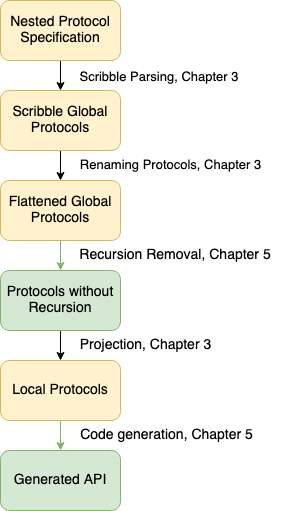
\includegraphics[scale=0.75]{figures/pipeline.png}
    \caption{Pipeline for Verification and API Generation of Nested Protocols}
    \label{project-pipeline}
\end{figure}

In Chapter 2, we introduce the typing discipline of session types and the current approach for generating the implementation of protocols from their session types using Scribble\cite{scribble}. We also describe the MPST theory of nested protocols which we use to develop our implemention.\\

In Chapter 3, we describe the extensions we have introduced to Scribble\cite{featherweight} in order to model nested protocols. We describe the new syntactic constructs we define based on the theory presented in \cite{nestedprotocols} and how we have extended the definitions in Scribble to take into the addition of nested protocols.\\

In Chapter 4, we discuss our design for the implementation of the Go APIs and the factors which have affected the choices we have made when coming up with this design. In particular, we describe how some of the features of Go, our target language have affected the approach we follow in our implementation and how we structure it.\\

In Chapter 5, we define the code generation scheme which we use to generate the different components in the implementation of nested protocols. We describe the correspondance between the different constructs of a Scribble protocol declaration and the implementation of the Go APIs. Developers can use the code that we generate to implement protocols which are correct by construction. The type system will guarantee that the messages will always be of the correct type and our implementation will ensure that the roles follow the behaviour specified by the protocol.\\

In Chapter 6, we evaluate our work through case studies implemented as nested protocols. We discuss the increase in expresiveness that nested protocols provide and evaluate the performance of our implementation design by running a benchmark on our case studies.\\

Finally, we conclude in Chapter 7 by outlining possible future improvements to our implementation and summarising our work.\\

Our work on extending Scribble with nested protocols has all been implemented on top of an existing OCaml implementation of the framework called \texttt{nuscr}\footnote{\href{https://github.com/nuscr/nuscr}{https://github.com/nuscr/nuscr}}. Our extension is currently only available a fork of the repository\footnote{\href{https://github.com/becharrens/nuscr}{https://github.com/becharrens/nuscr}}, but it should be integrated into the main repository once it has been reviewed and approved.

%The toolchain generates an implementation of the different roles in the protocol, allowing the user to define logic through callbacks. 
% \begin{figure}[tb]
% \centering
% 
\includegraphics[width = 0.4\hsize]{./figures/imperial}
% \caption{Imperial College Logo. It is nice blue, and the font is quite stylish. But you can choose a different one if you do not like it.}
% \label{fig:logo}
% \end{figure}

% Figure~\ref{fig:logo} is an example of a figure. 

%%%%%%%%%%%%%%%%%%%%%%%%%%%%%%%%%%%%
\chapter{Background}

\section{Session Types}
\subsection{Overview}

The two main models to reason about concurrent programs are shared memory and message passing. In shared memory, components communicate by reading and writing to a shared part of memory. This is how CPU threads and processes in a computer communicate with each other. However, reasoning about concurrent programs with this model can be tricky, as compiler and hardware optimisations can reorder the program's instructions\cite{sharedmemory}. On the other hand, in message passing inter-process communication is carried out by exchanging data in the form of explicit messages. This model closely resembles how communication is carried out in distributed systems.\\

Message passing can be encoded using the $\pi$-calculus, a process algebra based on name passing which was developed by Milner\cite{milnerpicalc}. In this calculus, processes communicate by sending channel names over named channels. We present an asynchronous variant of the $\pi$-calculus in section \ref{pi-calculus}. Session types\cite{binarysessiontypes1} introduce a typing discipline for formalising the communication exchanges between processes in the $\pi$-calculus. The initial theory was defined only for two participants, but it was later extended by Honda et al.\cite{asyncmpst1, asyncmpst2} to include multiple parties. This enabled the session types to encode a larger number of protocols. Session types improve the reliability of distributed systems by guaranteeing the correctness of the programs. If the processes are well-typed, they will have session fidelity and will not suffer from communication errors such as deadlocks, type mismatches or protocol violations.\\

There are already multiple implementations of session types for popular programming languages such as Java\cite{java}, C\cite{mpstc}, Go\cite{parametrictypes}, Python\cite{python}, Erlang\cite{erlang}, etc. Due to the set of features available to different programming languages, the implementation of MPST varies from one language to another. Some languages use rely on the type system to verify the correctness of the session's implementation at compile-time, while others may require run-time checks in order to detect protocol violations. 

\subsection{Asynchronous $\pi$-Calculus}\label{pi-calculus}
The $\pi$-calculus is a process algebra for encoding communicating systems. Processes communicate with one another through name passing, by sending and receiving channel names over named channels. The $\pi$-calculus is a simple yet powerful model which has been shown to be Turing-complete\cite{turingcomplete}, as it can encode the $\lambda$-calculus. The original theory was proposed by Robin Milner\cite{milnerpicalc}, but different variants have been proposed since. The first asynchronous $\pi$-calculus theory was presented in \cite{asyncandpicalc}, and we present a variant based on this theory, as defined in \cite{co406}.

\begin{figure}[h]
    \centering
    \begin{equation*}
    \centering
    \begin{array}{rrlcr}
        P,\ Q & ::= && \white & \text{Processes} \\[2.75pt]
             &   & 0 & \white & \text{Nil\ Process}  \\[2.75pt]
             & | & P\ |\ Q & \white & \text{Parallel\ Composition} \\[2.75pt]
             & | & (\nu\ a)\ P & \white & \text{Scope Restriction} \\[2.75pt]
             & | & !P & \white  & \text{Replication} \\[2.75pt]
             & | & \overline{u}\langle v \rangle & \white & \text{Output} \\[2.75pt] 
             & | & u(x).P & \white & \text{Input} \\\\
        u,\ v & ::= && \white & \text{Identifiers} \\[2.75pt]
              &   & a,\ b,\ c & \white & \text{Names} \\[2.75pt]
              & | & x,\ y,\ z & \white & \text{Variables} \\
        \end{array}
    \end{equation*}
    \caption{Syntax of monadic asynchronous  $\pi$-calculus}
    \label{picalc_syntax}
\end{figure}{}

The syntax of the asynchronous $\pi$-calculus is defined in Figure \ref{picalc_syntax}:
\begin{itemize}
    \item $0$ is the nil process, which represents the process with no actions.
    \item $P\ |\ Q$ is the parallel composition of two processes. These processes can execute in any order.
    \item $(\nu\ a)\ P$ is the scope restriction operation. It creates a new named channel $a$ that can only be used within process P and will not interfere with any other existing names.
    \item $!P$ is process replication. It represents the infinite parallel composition of process $P$: $P\ |\ P\ |\ P\ |\ ...$
    \item $\overline{u}\langle v \rangle$ is the output operation, which sends $v$ over $u$.
    \item $u(x).P$ is the input operation. It receives a a value over channel $u$. After receiving the value  it will continue executing process P, replacing all references to $x$ in $P$ with the received value.
\end{itemize}

Structural congruence is an equivalence relation which expresses that two processes are equivalent/interchangeable. We define the structural congruence of asynchronous $\pi$-calculus relation in Figure \ref{picalc_cong}.\\

\begin{figure}[h]
    \centering
    \begin{equation*}
    \centering
    \begin{array}{rcrclcr}
         & & P & \equiv & P & & \text{Reflexivity}\\[2.75pt]
         P \equiv Q & \implies & Q &\equiv\ & P & & \text{Symmetry}  \\[2.75pt]
         P \equiv Q\ \land\ Q \equiv R & \implies & P & \equiv & R & & \text{Transitivity} \\[2.75pt]
         P \equiv Q\ & \implies & (\nu\ a)\ P & \equiv & (\nu\ a)\ Q & & \text{Cong\ of\ Restriction} \\[2.75pt]
         P \equiv Q\ & \implies & P\ |\ R & \equiv & Q\ |\ R & & \text{Cong\ of\ Parallel\ Comp} \\[2.75pt]
         P \equiv Q & \implies & u(x).P & \equiv & u(x).Q & & \text{Cong\ of\ Input} \\[2.75pt]
         P \equiv Q & \implies & !P & \equiv & !Q & & \text{Cong\ of\ Replication} \\[2.75pt]
         P\ =_\alpha \ Q\ & \implies & P & \equiv & Q &  & \alpha-\text{equivalence} \\[2.75pt]
         & & P\ |\ (Q\ |\ R) & \equiv & (P\ |\ Q)\ |\ R & & \text{Associativity} \\[2.75pt]
         & & P\ |\ Q & \equiv & Q\ |\ P & & \text{Commutativity} \\[2.75pt]
         & & P\ |\ 0 & \equiv & P & & \text{Zero} \\[2.75pt]
         & & !P & \equiv & P\ |\ !P & & \text{Replication} \\[2.75pt]
         & & (\nu\ a)\ 0 & \equiv & 0 & & \text{Res\ of\ Nil} \\[2.75pt]
         & & (\nu\ a)(\nu\ b)\ P\ & \equiv & (\nu\ b)(\nu\ a)\ P & & \text{Res\ of\ Restriction} \\[2.75pt]
         a\ \notin\ fn(P) & \implies & \ P\ |\ (\nu\ a)\ Q & \equiv & (\nu\ a)(P\ |\ Q) & & \text{Res\ over\ Parallel\ Comp}
        \end{array}
    \end{equation*}
    \caption{Structural congruence of monadic asynchronous  $\pi$-calculus}
    \label{picalc_cong}
\end{figure}{}

The operational semantics of the $\pi$-calculus shown in Figure \ref{picalc_op_sem} define how the communication between the processes happens. The most important rule is \textsc{Comm}, which shows how the value sent by the output process is received by the input process and used in its continuation $P$ by replacing the references to the variable $x$ in $P$.

\begin{figure}[h!]
    \centering
    \begin{equation*}
    \centering
    \begin{array}{c}
    \inference{}{\overline{a}\langle v \rangle\ |\ a(x).P\ \longrightarrow\ P\{\sfrac{v}{x}\}}[\textsc{Comm}]\\[20pt]
    \inference{P\ \longrightarrow\ P'}{P\ |\ Q\ \longrightarrow\ P'\ |\ Q}[\textsc{Par}]\\[20pt]
    \inference{P\ \longrightarrow\ P'}{(\nu\ a)\ P \longrightarrow\ (\nu\ a)\ P'}[\textsc{Res}]\\[20pt]
    \inference{
        P \equiv Q 
        & Q\ \longrightarrow\ Q' 
        & Q' \equiv P'
    }{P\ \longrightarrow\ P'}[\textsc{Struct}]
    \end{array}
    \end{equation*}
    \caption{Operational semantics of monadic asynchronous $\pi$-calculus}
    \label{picalc_op_sem}
\end{figure}{}

It is important to notice that the output process $\bar{u} \langle v \rangle$ does not have any continuation. This reflects the asynchronous nature of the calculus. However, the asynchronous pi calculus presented above is very expressive; it is possible to encode other variants of $\pi$-calculus using it, including synchronous $\pi$-calculus, which permits continuation after output, and polyadic $\pi$-calculus, where it is possible to exchange vectors of messages at once. 

% The intuition for encoding synchronous $\pi$-calculus is to use two additional channels to agree on a rendez-vous between the sender and the receiver. The sender will send a channel over which to communicate, and the receiver will send a private channel over which the exchange will actually take place. To encode polyadic synchronous $\pi$-calculus using monadic synchronous pi cal, 

% \begin{table}[]
%     \centering
%     \begin{tabular}{l|p{6cm}|p{6cm}}
%          &$monadic\ asynchronous\ \longrightarrow\ monadic \ synchronous$ & $mondadic\ synchronous\ \longrightarrow\ polyadic\ synchronous$ \\
%          \hline
%          \textsc{Input} & $\llbracket \bar{u} \langle v \rangle.P$\rrbracket = \hfill (\nu\ c)(\bar{u} \langle c \rangle\ |\ c(y).(\bar{y} \langle v\rangle\ |\ \llbracket P \rrbracket))& $\llbracket \bar{u} \langle v \rangle.P$\rrbracket = \hfill (\nu\ c)(\bar{u} \langle c \rangle\ |\ c(y).(\bar{y} \langle v\rangle\ |\ \llbracket P \rrbracket))
         
%     \end{tabular}
%     \caption{Caption}
%     \label{tab:my_label}
% \end{table}{}

\subsection{Binary Session Types}
A session is a unit of conversation between participants. Session types provide a structured way to define and reason about the communications which take place between participants. In binary session types, these interactions happen between two participants. A session results from the binary composition of the processes of each participant. There are multiple similar formulations for session types in the literature, but Figure \ref{bst_session_calc} shows the syntax for processes in binary session types as presented in \cite{co406}. %presented in \textit{the CO406 course}\comment{replace with reference}.\\

\begin{figure}[h]
    \centering
    \begin{equation*}
    \centering
    \begin{array}{rrlcr}
        v & ::= & \underline{n} & \white & \text{Integers} \\[2.75pt]
              & |  & \texttt{true}\ |\ \texttt{false} & \white & \text{Booleans} \\[2.75pt]
              & | & \texttt{"str"} & \white & \text{Strings} \\\\
        e,\ e' & ::= & v & \white & \text{Values} \\[2.75pt]
              & |  & x & \white & \text{Variables} \\[2.75pt]
              & | & e\ +\ e'\ |\ e\ -\ e'\ |\ -e & \white & \text{Arithmetic} \\[2.75pt]
              & | & e\ =\ e'\ |\ e\ <\ e'\ |\ e\ >\ e' & \white & \text{Relational} \\[2.75pt]
              & | & e\ \land\ e'\ |\ e\ \lor\ e'\ |\ \lnot e & \white & \text{Logical} \\
              & | & e\ \bigoplus\ e' & \white & \text{Non-determinism}\\\\
        
        
        p & ::= & Alice\ |\ Bob & \white & \text{Participant}\\\\
        P,\ Q & ::= && \white & \text{Processes} \\[2.75pt]
             &   & 0 & \white & \text{Nil\ Process}  \\[2.75pt]
             & | & \overline{p} \langle e \rangle.P & \white & \text{Output} \\[2.75pt] 
             & | & p(x).P & \white & \text{Input}\\[2.75pt]
             & | & p\ \triangleright\ \{l_i:\ P_i\}_{i\in I}& \white & \text{Branching}\\[2.75pt]
             & | & p\ \triangleleft\ l.P& \white & \text{Selection} \\[2.75pt]
             & | & \texttt{if}\ e\ \texttt{then}\ P\ \texttt{else}\ Q & \white & \text{Conditional} \\[2.75pt]
             & | & \mu X.P & \white  & \text{Recursive}\ \text{Process} \\[2.75pt]
             & | & X & \white  & \text{Recursive\ Variable} \\\\
             
        M & ::= & p :: P\ |\ q :: Q & \white & \text{Binary\ Composition}
        \end{array}
    \end{equation*}
    \caption{Processes in the binary session calculus}
    \label{bst_session_calc}
\end{figure}{}

\begin{itemize}
    \item $0$ is the nil process, which represents no actions.
    \item $\overline{p} \langle e \rangle.P$ is the output operation, which sends the value $e$ to participant $p$ with continuation $P$ (the session calculus is synchronous).
    \item $p(x).P$ is the input operation, which waits for participant $p$ to send a value $x$. Upon receiving the value, execution continues with $P$, with the received value replacing the references to $x$ in $P$.
    
    \item $p\ \triangleright\ \{l_i:\ P_i\}_{i\in I}$ is the branching operation. The process waits for participant $p$ to send a label $l\ =\ l_i$, for some $i \in I$. After receiving the label, execution continues with process $P_i$.
    
    \item $p\ \triangleleft\ l.P$ is the selection operation. The process sends label $l$ to participant $p$, then continues executing $P$.
    
    \item $\texttt{if}\ e\ \texttt{then}\ P\ \texttt{else}\ Q$ is the conditional operation. Expression $e$ should evaluate to a boolean. If $e$ evaluates to true then process $P$ is executed, otherwise, $Q$ is executed.
    
    \item $\mu X.P$ and $X$ are used to express recursion in the processes. The recursive process $\mu X.P \equiv P\{\sfrac{\mu X.P}{X}\}$, that is, you are able to replace all the instances of the recursion variable $X$ in P with $\mu X.P$. This enables you to carry out potentially infinite unfoldings of the process.
    
    \item $e\ \bigoplus\ e'$ expresses a non-deterministic choice between two expressions of the same type, so the expression could evaluate to the result of either of the two expressions. 
    
    \item The evaluation of expressions is only defined when the types match: logical expressions are only defined on expressions which evaluate to booleans, arithmetic expressions and $e\ <\ e'$ and $e\ >\ e'$ are only defined on integer values, and $e\ =\ e'$ is only defined if $e$ and $e'$ have the same type.
\end{itemize}{}

This session calculus is based on the $\pi$-calculus, so we can observe a great amount of similarities between the constructs in both calculi. The main differences are the introduction of the branching and selection operations (which can be encoded in the $\pi$-calculus), the definition of recursion and the conditional process. \\

% The operational semantics for a session $M\ =\ p::P\ |\ q::Q$ are defined in a similar manner to the $\pi$-calculus. Additional rules are required for the branching/selection and the conditional processes. Reducing a recursive process may involve unfolding the recursion multiple times through structural congruence. For a formal definition please\\

We introduce the definition of the session types in Figure \ref{bst_session_types}. We will not give the formal typing judgements for the processes, these can be found in \cite{co406, binarysessiontypes1, subtyping}\comment{Course material ref and possibly language primitives}. However, we give an intuition behind the correspondence between processes and their session types:

\begin{figure}[h]
    \centering
    \begin{equation*}
    \centering
    \begin{array}{rrlcr}
        S & ::= && \white & \text{Session\ Type} \\[2.75pt]
             &   & \texttt{end} & \white & \text{Termination}  \\[2.75pt]
             & | & p![U];\ S & \white & \text{Value\ Send} \\[2.75pt]
             & | & p?[U];\ S & \white & \text{Value\ Receive} \\[2.75pt]
             & | & p \bigoplus \{l_i\ :\ S_i\}_{i \in I} & \white& \text{Selection} \\[2.75pt]
             & | & p \& \{l_i\ :\ S_i\}_{i \in I} & \white & \text{Branching} \\[2.75pt] 
             & | & t & \white & \text{Type\ Variable} \\[2.75pt]
             & | & \mu t.S & \white & \text{Recursive\ Type}\\\\
        U & ::= & \texttt{int}\ |\ \texttt{bool}\ |\ \texttt{string}& \white & \text{Sorts\ for\ Expressions}
        \end{array}
    \end{equation*}
    \caption{Syntax of binary session types}
    \label{bst_session_types}
\end{figure}{}

\begin{itemize}
    \item $Bob(x).\overline{Bob} \langle x + 1 \rangle.0:\ Bob?[\texttt{int}];\ Bob![\texttt{int}];\ \texttt{end}$ - In order to infer the sort of the input variable it may be necessary to see how it is used in the process.
    \item $Alice\ \triangleleft\ choice.\overline{Alice} \langle \texttt{"hello"} \rangle.0:\ Alice \bigoplus \{choice:\ Alice![\texttt{str}];\ \texttt{end}\}$ - similarly for branching.
    \item In order to be able to specify a type for a conditional process $\texttt{if}\ e\ \texttt{then}\ P\ \texttt{else}\ Q$, both branches $P$ and $Q$ must have the same type $S$, and therefore the type of the conditional process will also $S$.
    \item $\mu t.S$ and $t$ are used to specify recursive types. They work much in the same way as recursive processes; recursive types can also unfolded by replacing instances of $t$ in $S$ by $\mu t.S$.
\end{itemize} 

\begin{figure}[h!]
    \centering
    \begin{equation*}
    \centering
    \begin{array}{rcl}
             \overline{\texttt{end}} & = & \texttt{end}  \\[2.75pt]
             \overline{p![U];\ S} & = & p?[U];\ \overline{S} \\[2.75pt]
             \overline{p?[U];\ S} & = & p![U];\ \overline{S} \\[2.75pt]
             \overline{p \bigoplus \{l_i\ :\ S_i\}_{i \in I}} & = & p \& \{l_i\ :\ \overline{S_i}\}_{i \in I}\\[2.75pt]
             \overline{p \& \{l_i\ :\ S_i\}_{i \in I}} & = & p \bigoplus \{l_i\ :\ \overline{S_i}\}_{i \in I}\\[2.75pt]
             \overline{\mu t.S} & = & \mu t.\overline{S}\\[2.75pt]
             \overline{t} & = & t
        \end{array}
    \end{equation*}
    \caption{Duality of binary session types}
    \label{bst_duality}
\end{figure}{}

A key concept in binary session types is duality. When two processes are composed in a session, in order for the session to progress correctly, both processes must be carrying out complimentary operations. For instance, if $Alice$ is trying to send a string to $Bob$, $Bob$ must be waiting to receive a string from $Alice$, otherwise the protocol is stuck. Similarly, if $Bob$ is waiting for a label from $Alice$ to decide which branch to execute, $Alice$'s process must send one of the expected labels. Not only must the constructs be complimentary, but the types of the messages being sent must also match. Therefore, in order for a session to be correct, the processes involved must be duals of one another. This will ensure that the binary session will always make progress and that the session continues to be well-typed as the protocol is carried out. The duality of binary session types is shown in Figure \ref{bst_duality}.



\subsection{Multiparty Session Types}\label{multiparty-session-types}
Binary session types have limited applications to real-world problems, as standard protocols tend to be much more complex and involve more than two participants. These interactions cannot always be correctly expressed as the composition of binary sessions between different pairs of participants. \\

Multiparty session types\cite{asyncmpst2} extend the theory to enable protocols to have multiple participants, thus overcoming these limitations. The main idea is to introduce global types, which describe the multiparty interactions within a protocol from a global perspective, as well as deriving a specification of the behaviour of each participant as local session type through the projection operation. \\

There are multiple variants of processes and their respective MPST in the literature. We present the syntax for synchronous multiparty session types defined in \cite{verygentleintrotompst} in Figure \ref{MPST_processes}.

\begin{figure}[h]
    \centering
    \begin{equation*}
    \centering
    \begin{array}{rrlcr}
        P,\ Q & ::= && \white & \text{Processes} \\[2.75pt]
             &   & 0 & \white & \text{Nil\ Process}  \\[2.75pt]
             
             & | & \texttt{if}\ e\ \texttt{then}\ P\ \texttt{else}\ Q & \white & \text{Conditional} \\[2.75pt]
             & | & \mu X.P & \white  & \text{Recursive}\ \text{Process} \\[2.75pt]
             & | & X & \white  & \text{Recursive\ Variable}\\[2.75pt]
             & | & p!l \langle e \rangle.P & \white & \text{Output} \\[2.75pt]
             & | & \sum\limits_{i \in I} p?l_i(x_i).P_i & \white & \text{Branching} \\\\

        M & ::= &&& \text{Multiparty\ Session}\\[2.75pt]
        & | & p :: P\ & \white & \text{Process}\\[2.75pt]
        & | & M\ |\ M\ & \white & \text{Parallel\ Composition}\\\\
        
        &&p,\ q,\ r,\ ... & \white & \text{Participants}\\[2.75pt]
        &&e,\ e',\ ... & \white & \text{Expressions}\\[2.75pt]
        &&x,\ y,\ z,\ ... & \white & \text{Expression\  variables}
        \end{array}
    \end{equation*}
    \caption{Processes in multiparty session calculus}
    \label{MPST_processes}
\end{figure}{}

Although the syntax has some minor difference when compared to the one showed in Figure \ref{bst_session_calc}, the semantics are essentially the same. The main difference is that processes now send/receive a label with the value they communicate. Because sessions now involve multiple participants, it is necessary to specify the other participant for the exchange (it would have been possible to omit this information in binary session types). \\

In multiparty session types, when deriving the types for protocols we consider both the global type, which formally specifies the interactions between all the participants in the protocol from a global perspective and local session types, which characterize the interactions that each of the participants carry out within the global protocol. The parallel composition of processes satisfying the session types implements the behaviour of the global type. In this way, the implementations of the different participants are decoupled from one another, so they could be implemented separately and the overall implementation would be correct as long as they all follow their respective session types.

\begin{figure}[h]
    \centering
    \begin{equation*}
    \centering
    \begin{array}{rrlcr}
        S & ::= & \texttt{int}\ |\ \texttt{bool}\ |\ \texttt{string}& \white & \text{Sorts}\\\\
        \textsc{Global\ Types} & && &\\[3pt]
        G & ::= & \texttt{end} & \white & \text{Termination}  \\[2.75pt]
             & | & p \longrightarrow q: \{l_i( S_i).G_i\}_{i \in I} & \white & \text{Branching} \\[2.75pt] 
             & | & t & \white & \text{Type\ Variable} \\[2.75pt]
             & | & \mu t.G & \white & \text{Recursive\ Type}\\\\
             
        \textsc{Local Types} &&&& \\[3pt]
        T & ::= & \texttt{end} & \white & \text{Termination}  \\[2.75pt]
          & | & \bigoplus_{i \in I}\ p!l_i(S_i).T_i & \white& \text{Selection} \\[2.75pt]
          & | & \&_{i \in I}\ p?l_i(S_i).T_i & \white & \text{Branching} \\[2.75pt] 
          & | & t & \white & \text{Type\ Variable} \\[2.75pt]
          & | & \mu t.S & \white & \text{Recursive\ Type}
        
        \end{array}
    \end{equation*}
    \caption{Syntax of multiparty session types}
    \label{MPST_types}
\end{figure}{}

We present the syntax for global and local types in Figure \ref{MPST_types}. Similarly to the syntax of processes, the local session types are almost the same as the binary session types. Global types introduce a single construct for branching/selection, $p \longrightarrow q:\{l_i(S_i).G_i\}_{i \in I}$, in which participant $p$ sends to $q$ the label (and corresponding value) which will determine what the continuation is.\\

Each participant in the protocol enacts a role in the global type. The session type for each role is derived by projecting the global type onto that role, which essentially ignores all the interactions in which the role does not take part, leaving only the behaviour that needs to be implemented for that role within the protocol. The projection operation is defined in Figure \ref{MPST_projection}.\\

\begin{figure}[h]
    \centering
    \begin{equation*}
    \centering
    \begin{array}{rcl}
        
        (p \longrightarrow p':\{l_i(S_i).G_i\}_{i \in I}) \upharpoonright q & = &
        \begin{cases}
            \bigoplus_{i \in I}\ p'!l_i(S_i).(G_i \upharpoonright q) & \text{if}\ q\ =\ p\\
            \&_{i \in I}\ p?l_i(S_i).(G_i \upharpoonright q) & \text{if}\ q\ =\ p'\\
            G_{i_0} \upharpoonright q & \text{where}\ i_0 \in I,\ \text{if}\ q \notin \{p,\ p'\}\\
            & \text{and}\ \forall i,j \in I.\ G_i \upharpoonright q\ =\ G_j \upharpoonright q
        \end{cases}\\[33pt]
        (\mu t.G) \upharpoonright q & = & 
        \begin{cases}
            \mu t.(G \upharpoonright q) & \text{if}\ G \upharpoonright q \neq t\\
            \texttt{end} & \text{otherwise}
        \end{cases}\\[13pt]
        t \upharpoonright q & = & t\\[2.75pt]
        \texttt{end} \upharpoonright q & = & \texttt{end}\\[2.75pt]
        \end{array}
    \end{equation*}
    \caption{Projection of Global Types to Local Types}
    \label{MPST_projection}
\end{figure}{}

Projecting a role $q$ on $\texttt{end}$ and $t$ (type variable) has no impact, since $q$ is not participating in any exchange. When projecting on $p \longrightarrow p':\{l_i(S_i).G_i\}_{i \in I}$, depending on which role $q$ is undertaking in the exchange, the projected session type will change. 
\begin{itemize}
    \item If the $q = p$, then the projection is a selection, as the process decides which label and value to send to $p'$. The continuations $G_i$ must be projected onto $q$ as well.
    \item Similarly, if $q = p'$, $q$ will be waiting for a message from $p$, therefore the projected session type is a branching operation. 
    \item  When $q$ does not participate in the label exchange, the projection becomes more tricky. There are multiple approaches to resolve this situation; the one shown in Figure \ref{MPST_projection} is known as plain merge. Since $q$ does not know which branch will have been chosen by $p$, all branches must have the same continuation from $q$'s viewpoint, otherwise $q$ would not know which behaviour to implement. A different approach called the full merge provides a less restrictive definition\cite{verygentleintrotompst}.
    
\end{itemize}

In binary session types, ensuring that both participants implemented session types which were duals of one another was enough to guarantee the correctness of the protocol. With multiple participants however, that is not the case anymore. Although you can ensure that each pair of participants has dual interactions, in order to guarantee the correctness that alone is not enough. The projection operation ensures that the composition of the different local types produced satisfies the global type. Multiparty session types can therefore provide many guarantees about the communication of well-typed multiparty sessions such as:
\begin{itemize}
    \item \textbf{Progress}: A multiparty session $M$ can either have ended ($M\ \equiv\ p :: 0$) or it can continue to execute (there exists $M'$ such that $M \longrightarrow M'$). This means that every sent message will eventually be received and every process waiting for a message eventually receives one. \cite{verygentleintrotompst, gentleintrotompst}
    \item \textbf{Subject reduction}: If a well-typed session $M:\ G$ reduces to $M'$, then $M':\ G'$ is well typed\cite{verygentleintrotompst}.
    \item \textbf{Type Safety}: If $M:\ G$ is well-typed then the session will never get stuck - a session where there are processes which have not finished must able to continue executing\cite{verygentleintrotompst}.
    \item \textbf{Protocol fidelity}: All interactions which happen are expressed in the global type of the protocol\cite{gentleintrotompst}.
    \item \textbf{Communication Safety}: There can never be a mismatch between the types of messages which are sent and which are expected\cite{gentleintrotompst}.
\end{itemize}{}

\subsection{Scribble API Endpoint Generation}\label{Scribble}
Scribble\cite{scribble,featherweight} is a protocol description language based on multiparty session types. The Scribble framework translates this formal definition of the protocol into an implementation in one of various programming languages, thus applying the theory of MPST in a practical setting. A protocol describes the structure of the message exchanges between different roles, the entities which will participate in the protocol.\\

We present the syntax of the Scribble language as defined in \cite{featherweight} in Figure \ref{scribble-global-protocol}. A Scribble module can contain multiple protocols, with one of them being the designated point of entry for the computation. Protocols can call each other through the $\scrdo$ construct, but this essentially corresponds to inlining the called protocol. In order for a protocol call to be valid, it must be called with number of roles specified in its declaration. The remaining syntactic constructs relate closely to the different session types in the theory, described in Section \ref{multiparty-session-types}. A message exchange is specified by the label of the message and the type of its payload, \texttt{S}, and the sender and receiver roles. Although here we only specify one payload type there could potentially be zero or more multiple ones. Some implementations of Scribble also permit the user to optionally specify names for each of the payload fields, but we omit this in our notation as well. The $\choice$ construct encodes the external choice by a role, with a set of the different continuations which can happen based on the role's choice. The recursive type and type variables are directly encoded by the $\rec$ and $\continue\ t$ constructs, and the \texttt{end} session type is represented with the $\scrend$ construct.\\



\begin{figure}[!h]
    \centering
    \begin{math}
        \begin{array}{rcl}
            \mathit{Module} & ::= & \mathit{P}+\\\\
            \mathit{P} & ::= & \scrglobal\ \protocol\ \mathit{pro}(\rolessig{A}{n})\ \{\;\mathit{G}\;\} \\\\
            % G & ::= & \texttt{end} & \white &
            \mathit{G} & ::= &\\[2.75pt]
              &   | & \choice\ \at\ \mathit{A}\ \{\;\mathit{G_1}\;\}\ \scror\ ...\ \scror\ \{\;\mathit{G_n}\;\} \\[2.75pt]
              &   | & \scrmessage{a}{S}\ \from\ \mathit{A}\ \scrto\ \mathit{B};\ \mathit{G} \\[2.75pt]
              &   | & \rec\ \mathit{t}\ \{\;G\;\} \\[2.75pt]
              &   | &  \continue\ \mathit{t} \\[2.75pt]
              &   | & \scrdo\ \mathit{pro}(\roles{A}{n});\ \mathit{G} \\[2.75pt]
              &   | & \scrend \\[2.75pt]
        \end{array}
    \end{math}
    \caption{Syntax of Scribble global protocols}
    \label{scribble-global-protocol}
\end{figure}

A syntactically correct protocol where all the protocol calls are valid can be expanded with the interactions of the called protocols to produce a single large protocol with all the interactions which must be performed. Scribble the verifies that the protocol is well-formed, which ensures local protocols can be generated for all the roles. Syntactically correct protocols can be ambiguous, for instance, if the first message in two branches of a $\choice$ have the same signature, as other roles would not be able to tell which branch has been chosen. The local protocols are derived by projecting the global type onto each of the roles. A communication finite state machine (CFSM) is then generated for each of the local protocols, which expresses the valid transitions between states that a role can carry out during the protocol. These transitions represent a message exchange with a different participant.\\

An example of a global protocol can be seen in Figure \ref{scribble_protocol}, which shows a calculator protocol carried out by two roles: a client who enters the operands and the server who carries out the operation. The protocol has a recursive loop in which the client can choose to either send two numbers to multiply to the server, get the result back and start over again or quit the protocol. The resulting CFSM for the server $S$ can be seen in Figure \ref{scribble_fsm}.\\

\begin{figure}[h]
    \centering
    \lstset{language=Scribble}
    \begin{lstlisting}
global protocol Calc(role S , role C ) {
    rec Loop {
    	choice at C {
    		multiply(int, int) from C to S;
    		result(int) from S to C ;
    		continue Loop ;
    	} or {
    		quit() from C to S ;
    		terminate() from S to C ;
    	}
    }
}
    \end{lstlisting}
    \caption{Calculator Protocol}
    \label{scribble_protocol}
\end{figure}{}

\begin{figure}[h!]
    \centering
    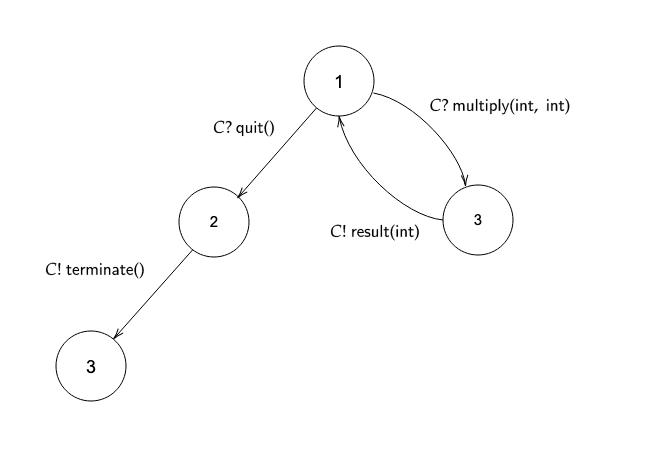
\includegraphics[scale=0.53]{scribble_fsm.png}
    \caption{CFSM for role S in Calculator Protocol}
    \label{scribble_fsm}
\end{figure}{}
We describe how the CFSMs can be used to generate code in an OOP programming language like Java for the different endpoints (roles) in the protocol. Each of the states in the CFSM is converted to a class with methods for each of the outgoing transitions from the current state, which carry out the necessary communication operations and return the next state. The user can chain calls to these methods to carry out the protocol, transitioning only between valid states until the final state is reached, which does not have any outgoing transitions. \\

In order to ensure the correctness of the implementation, every state must only be used once, which may require run-time checks. Implementations using the Scribble-generated APIs benefit from the correctness guarantees of MPST, ensuring that there are no communication errors and that the protocol is followed properly.\\

\section{Nested Protocols}
\subsection{Motivations}
The theory of session types has been extended in different directions in order to be able to become more expressive. Some advances have made it possible to annotate the protocol with logical assertions to define extra properties that the protocol should meet\cite{logicaassertions}. Other developments have made it possible to express protocols with parametrised roles\cite{parametrictypes} (expressing protocols where $n$ participants carry out particular roles), or to have greater control over how participants can join or leave a session through a dynamic multiparty session\cite{multirolesessiontypes}. \\

Demangeon and Honda \cite{nestedprotocols} try to address a different challenge: protocols used in networking and in distributed systems are increasingly large. In many cases, they are highly modular, and often different protocols share the same structure. In order to better define and manage these protocols they extend the theory of session types to include nested protocols, which make it possible to define complex protocols using a simpler modular structure. Using this approach, protocols which have a similar structure can be grouped together under a single parametrised protocol, and complex protocols which might call other protocols can be expressed by making a call to those subprotocols. Moreover, different calls to the same subprotocol can be made with different parameters to achieve different behaviours. In their theory, subprotocols can also bring in new participants by `inviting' them to participate. This can help simplify some protocols, as it enables you specify protocols where participants are brought in/contacted only if required.

\subsection{Nested Session Calculus}
The theory they proposed is based on the idea of nesting protocols, where a parent protocol may define independent subprotocols and call them during its execution. Calls to a protocol can pass in different kinds of arguments as parameters such as values, roles from the parent protocol which will participate in the subprotocol and even other protocols which might be used during the call, similar to higher-order functions in functional programming.\\ 

Subprotocols are implemented as subsessions. The participant calling the protocol will create a new private session for its execution, and will send \textit{internal invitations} to all the roles in the parent protocol which will participate, and \textit{external invitations} to bring in new agents. In this way, only the roles which have a access to the subsession, so the other roles in the parent session will not be able to interfere with it. This model thus makes it possible to have private interactions in a public session. Using the Scribble language described in Section \ref{Scribble}, it is also possible to define subprotocols, but as opposed to this theory, the roles participating in Scribble protocols have to be known statically, meaning that a protocol call corresponds to inlining the subprotocol.\\

Calling subprotocols also abstract away their actual implementation, which means that the implementation of the subprotocol can be changed (e.g. to change how authentication is carried out or to improve the protocol's security) without changing the implementation of the parent protocol. Subprotocols also give a better separation between the different execution branches of the protocol, as different external participants can be invited only when required, reducing the complexity and utilisation of resources. For instance, in an HTTP-like protocol a proxy could have the choice of either returning a cached response directly or to initiate a \textit{Contact} protocol to involve the server and get the response. \\

\begin{figure}[h]
    \centering
    \begin{equation*}
    \centering
    \begin{array}{rrlcr}
        P,\ Q & ::= && \white & \text{Processes} \\[2.75pt]
             &   & 0 & \white & \text{Nil\ Process}  \\[2.75pt]
             & | & P\ |\ Q & \white & \text{Parallel\ Composition}  \\[2.75pt]
             & | & a(x).P & \white & \text{Receive\ Ext.\ Invitation} \\[2.75pt]
             & | & \overline{a}\langle s \rangle.P & \white & \text{Send\ Ext.\ Invitation} \\[2.75pt]
             & | & P\ +\ P & \white & \text{Non-determinism}\\[2.75pt]
             & | & k?[r, r]_{i \in I} \{l_i(x_i).P_i\}& \white & \text{Branching} \\[2.75pt]
             & | & k![r, r]l \langle v \rangle.P & \white & \text{Selection} \\[2.75pt]
             & | & (\nu\ u)\ P & \white & \text{Scope\ Restriction}\\[2.75pt] 
             & | & \texttt{new}\ s\ \texttt{on}\ k\ \texttt{with}\ (\widetilde{v})\&(\widetilde{a}\ \texttt{as}\ \widetilde{r}).P & \white & \text{Subprotocol\ Call}\\[2.75pt]
             & | & s \downarrow [r,\ r_1 : r_2](x).P & \white & \text{Receive\ Internal\ Invitation}\\[2.75pt]
             & | & s \uparrow [r,\ r_1 : r_2]\langle s \rangle.P & \white & \text{Send\ Internal\ Invitation}\\[2.75pt]
             & | & \mu X(x).P\langle v \rangle & \white  & \text{Recursive\ Process} \\[2.75pt]
             & | & X\langle v \rangle & \white  & \text{Recursive\ Variable}\\\\

        % M & ::= &&& Multiparty\ Session\\[2.75pt]
        % & | & p :: P\ & \white & Process\\[2.75pt]
        % & | & M\ |\ M\ & \white & Parallel\ Composition\\\\
        &&s,\ k,\ ... & \white & \text{Session\ names}\\[2.75pt]
        &&a,\ b,\ u,\ ... & \white & \text{Shared\ channels}\\[2.75pt]
        &&v & \white & \text{Values}\\
        &&r,\ r',\ ... & \white & \text{Role\ Identifiers}\\[2.75pt]
        &&x,\ y,\ z,\ ... & \white & \text{Variables}
        \end{array}
    \end{equation*}
    \caption{Processes in Session Calculus for Nested Protocols}
    \label{nested_session_calculus}
\end{figure}{}

Figure \ref{nested_session_calculus} shows the session calculus presented in the paper which includes the syntax for invitations and defining protocols. The calculus is based on the $pi$-calculus and shares a lot of the constructs of other existing session calculi\cite{logicaassertions}. Names are divided into two kinds: session channels, which handle all exchanges within a session, and shared channels, used to send and receive external invitations. 
\begin{itemize}
    \item Parallel composition, scope restriction and the nil process are defined as before.
    \item Recursion is also defined in a similar way as before, but it can additionally pass in a value to the recursive call which may be used when the recursive call is expanded. 
    \item $a(x).P$ and $\overline{a}\langle s \rangle.P$ are used for receiving and sending external invitations over the shared channel $a$.
    \item $P\ +\ P$ is the non-deterministic process. Execution can continue with either one of the two processes.
    \item $k?[r_1, r_2]_{i \in I} \{l_i(x_i).P_i\}$ is the branching operation from $r_1$ to $r_2$ with continuation $P_i$ in session $k$. $k![r_1, r_2]l \langle v \rangle.P$ is the selection operation, its dual primitive. 
    \item $s \downarrow [r,\ r_1 : r_2](x).P$ is the action for waiting for an internal invitation sent by $r$ to $r_1$ in order to play role $r_2$ in session $s$. 
    \item $s \uparrow [r,\ r_1 : r_2]\langle s \rangle.P$ is the action of sending an invitation from $r$ to $r_1$ in order to play role $r_2$ in session $s$.
    \item $\texttt{new}\ s\ \texttt{on}\ k\ \texttt{with}\ (\widetilde{v})\&(\widetilde{a}\ \texttt{as}\ \widetilde{r}).P$ is the operation for calling a subprotocol. Creates a new subsession $s$ within the parent session $k$, passing in arguments $\widetilde{v}$ and using shared channels $\widetilde{a}$ to send the external invitations.
\end{itemize}

\subsection{Nested Session Types}\label{nested-session-types}
The paper also extends the syntax of session types to include the types for defining and calling subprotocols as well as sending and receiving invitations. The extended syntax for local and global types is shown in Figure \ref{nested_session_types}. They define kinds (types for types), including $\diamond$, which represents the protocol type, in order to formalize the definition of protocols. The definition of global types is essentially the same as before:
\begin{itemize}
    \item Termination, branching and recursion are almost the same as before. They also define the type for parallel composition.
    \item They introduce the construct $G_1\ \bigoplus^r\ G_2$ to represent located choice, where role $r$ can choose between two different branches. 
    \item $\texttt{let}\ \mathcal{P}\ =\ \lambda\widetilde{r}^1,\ \widetilde{y} \mapsto \texttt{new}\ \widetilde{r}^2.G\ \texttt{in}\ G'$ defines a subprotocol $\mathcal{P}$. The vector of roles $\widetilde{r}^1$ defines a set of roles that will be carried out by roles from the parent protocol which will be internally invited, whereas the vector $\widetilde{r}^2$ contains the set of roles which will be externally invited. The protocol also takes in vector of values $\widetilde{y}$.
    \item $r\ \texttt{calls}\ \mathcal{P}\langle \widetilde{r},\ \widetilde{y}\rangle.G$ is the subprotocol call carried out by role $r$, internally inviting roles $\widetilde{r}$ and passing in the values $\widetilde{y}$.
\end{itemize}{}

The local session types have the same constructs as before, as well as the new constructs to handle invitations and protocol calls:
\begin{itemize}
    \item Termination, branching, selection and recursion are almost unchanged, and they introduce a type for parallel composition. 
    \item The construct $T_1\ \bigoplus^r\ T_2$ represents located choice.
    \item $\texttt{call}\ \mathcal{P}:G\ \texttt{with}\ (\widetilde{v}\ \texttt{as}\ \widetilde{y}:\widetilde{S})\&(\widetilde{r}^2).T$ is a call to the subprotocol $\mathcal{P}$, which has global type $G$, sending a vector of values $\widetilde{v}$ as arguments with sorts $\widetilde{S}$ and externally inviting the roles in $\widetilde{r}^2$ to participate in the subprotocol.
    \item Sending and accepting invitations for a role $r$ are handled by the $\texttt{req}\ \mathcal{P}[r]\langle \widetilde{v} \rangle\ \texttt{to}\ r.T$ and $\texttt{ent}\ \mathcal{P}[r]\langle \widetilde{v} \rangle\ \texttt{from}\ r.T$ constructors respectively.
\end{itemize}{}

\begin{figure}[h]
    \centering
    \begin{equation*}
    \centering
    \begin{array}{rrlr}
        Val & ::= & \texttt{int}\ |\ \texttt{bool}\ |\ \texttt{string} & \text{Sorts}\\\\
        K, S & ::= & Role\ |\ Val\ |\ \diamond\ |\ (K_1\ \times\ ...\ \times\ K_n) \longrightarrow K & \text{Kinds}\\\\
        
        \textsc{Global\ Types} & & &\\[3pt]
        G & ::= & \texttt{end} & \text{Termination}  \\[2.75pt]
             & | & \texttt{let}\ \mathcal{P}\ =\ \lambda\widetilde{r}^1,\ \widetilde{y} \mapsto \texttt{new}\ \widetilde{r}^2.G\ \texttt{in}\ G' & \text{Subprotocol\ Def}\\[2.75pt]
             & | & r\ \texttt{calls}\ \mathcal{P}\langle \widetilde{r},\ \widetilde{y}\rangle.G  & \text{Subprotocol\ Call} \\[2.75pt]
             & | & r_1 \longrightarrow r_2: \sum_{i \in I}\{l_i( S_i).G_i\} &  \text{Branching} \\[2.75pt]
             & | & G_1\ \bigoplus^r\ G_2   & \text{Located Choice} \\[2.75pt]
             & | & G_1\ |\ G_2 & \text{Parallel\ Composition} \\[2.75pt]
             & | & t & \text{Type\ Variable}\\[2.75pt]
             & | & \mu t.G & \text{Recursive\ Type}\\\\
             
        \textsc{Local Types} &&& \\[3pt]
        T & ::= & \texttt{end} &  \text{Termination}  \\[2.75pt]
          & | & \texttt{send}[r]!_{i \in I}\{ l_i(x_i: S_i).T_i\} & \text{Selection} \\[2.75pt]
          & | & \texttt{get}[r]?_{i \in I}\{l_i(x_i:S_i).T_i\} &  \text{Branching} \\[2.75pt] 
          & | & T_1\ \bigoplus \ T_2   & \text{Located Choice} \\[2.75pt]
          & | & T_1\ |\ T_2 & \text{Parallel\ Composition} \\[2.75pt]
          & | & \texttt{call}\ \mathcal{P}:G\ \texttt{with}\ (\widetilde{v}\ \texttt{as}\ \widetilde{y}:\widetilde{S})\&(\widetilde{r}^2).T &  \text{Subprotocol Call} \\[2.75pt]
          & | & \texttt{ent}\ \mathcal{P}[r]\langle \widetilde{v} \rangle\ \texttt{from}\ r.T &  \text{Accept Invitation} \\[2.75pt]
          & | & \texttt{req}\ \mathcal{P}[r]\langle \widetilde{v} \rangle\ \texttt{to}\ r.T &  \text{Send Invitation} \\[2.75pt]
          & | & t &  \text{Type\ Variable} \\[2.75pt]
          & | & \mu t.T &  \text{Recursive\ Type}
        
        \end{array}
    \end{equation*}
    \caption{Syntax of Session Types for Nested Protocols}
    \label{nested_session_types}
\end{figure}{}

As before, deriving the local types from the global type is done through the projection operation, although now it becomes necessary to define a protocol environment to hold the types of the nested protocols, which gets updated by the $let\ in$ constructor.\\ 

Figure \ref{nested_session_projection} shows the definition of projection for the nested protocol definition and call. Projection on the remaining constructors is defined in the standard way. Projection of a protocol definition updates the environment with the protocol's global type and signature and continues recursively projecting the type. When projecting a nested protocol call onto a role $r^p$, there are multiple cases to consider:
\begin{itemize}
    \item if $r^p$ is the caller but does not participate itself in the subprotocol, the projection must only send out the internal invitations in parallel, as well as executing the projection of the continuation.
    \item if $r^p$ is the caller as well as a participant, then it must also send all the internal invitations to all the participating roles, but that includes itself, it must also accept its own invitation.
    \item if $r^p$ did not call the protocol but is a participant of the protocol, then it must simply accept the invitation, with the continuation being the projection of the continuation of the global type.
    \item otherwise, $r^p$ is neither a participant or the caller, so the projection is the projection of the continuation of the global type.
\end{itemize}

\begin{figure}[h]
    \centering
    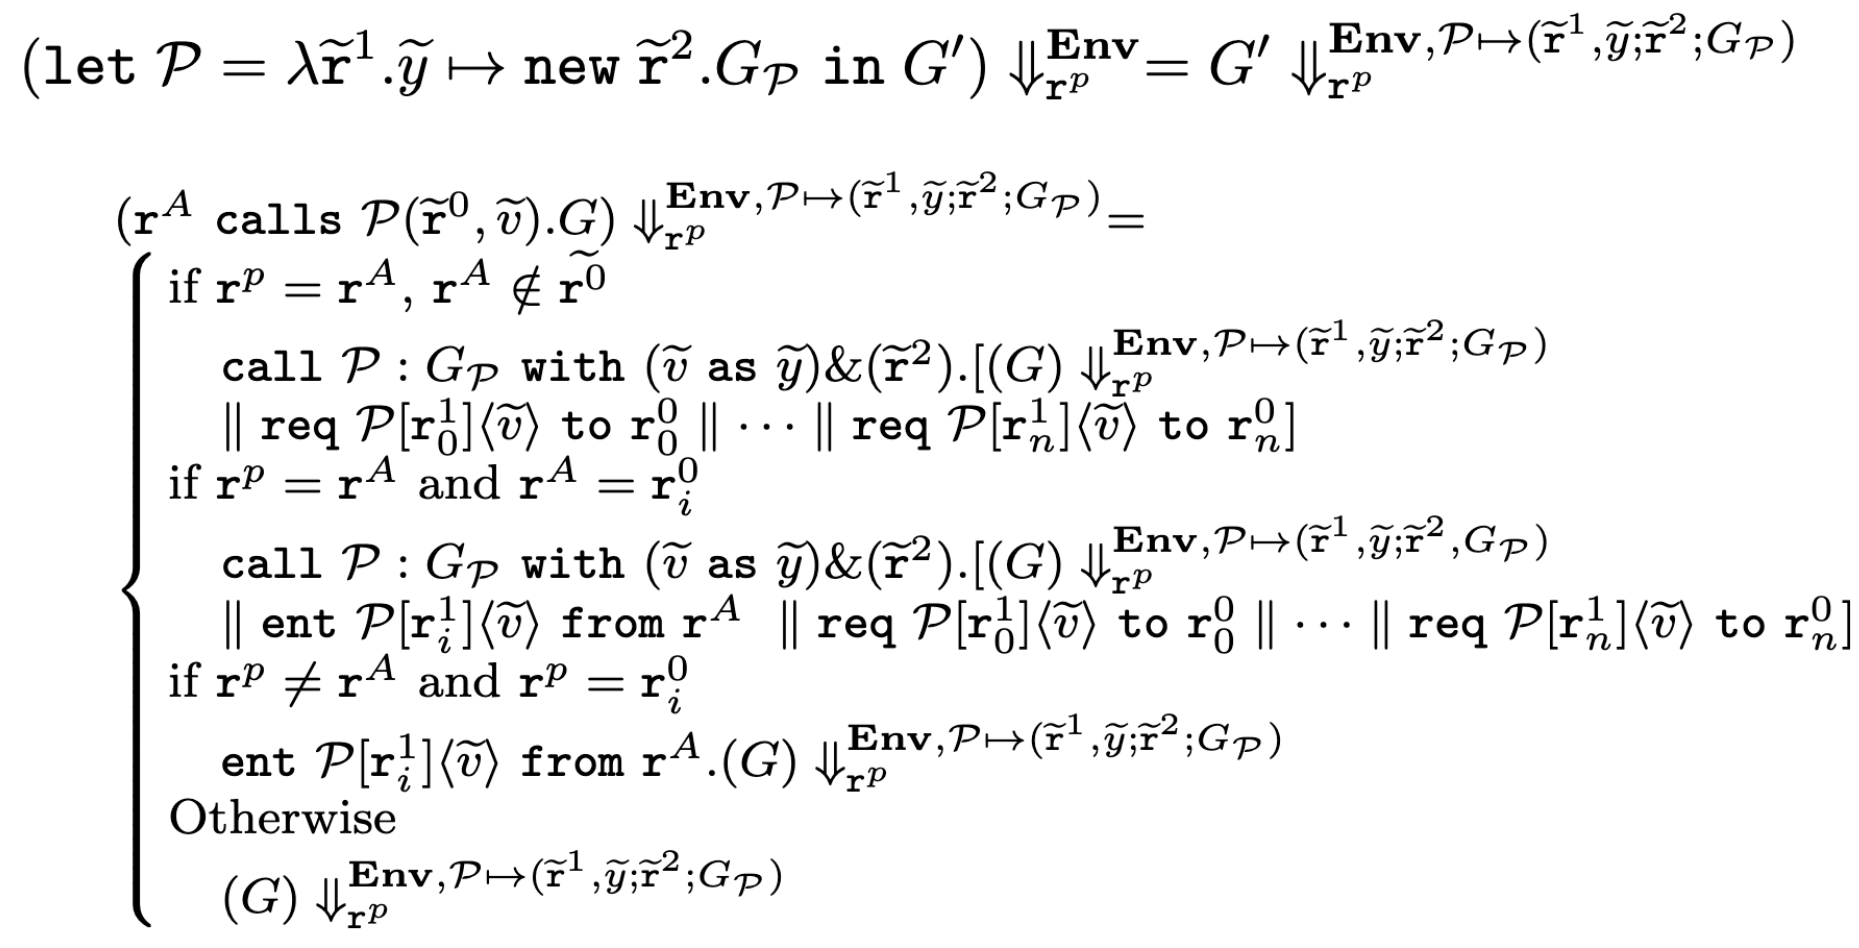
\includegraphics[scale=0.45]{nested_session_projection.png}
    \caption{Projection of Global Type in Nested Protocols\cite{nestedprotocols}}
    \label{nested_session_projection}
\end{figure}{}

\subsection{Returning Values from Subprotocols}\label{nested-protocols-return-value}
One limitation of the formulation expressed above is the inability of communication from a subsession back to the parent subsession. This means that it is impossible to express in a session type the relationship between a value calculated during a subsession and a value which a role might send after the nested protocol has ended. \\

For example, in the Client-Proxy-Server protocol described in Figure \ref{nested_session_example}, the value the server returns is $ans$, but that value cannot be seen outside of the $Contact$ subprotocol, so the proxy (middle) can only return $ans_0$ after completing the call to $Contact$. However, there are no guarantees that these two values are the same. The paper proposes some further extensions to the syntax of session types in order to make the protocol end by returning a value to the role which initiated the call in order to be able to capture be able to return information from the subprotocol. \\

Nevertheless, the current theory will suffice in most scenarios, as the kinds of the messages alone restrict what values can be sent, and it is up to the user's implementation to decide which value to send. Any value which satisfies this constraint can be considered a valid implementation of the protocol.
\begin{figure}[h]
    \centering
    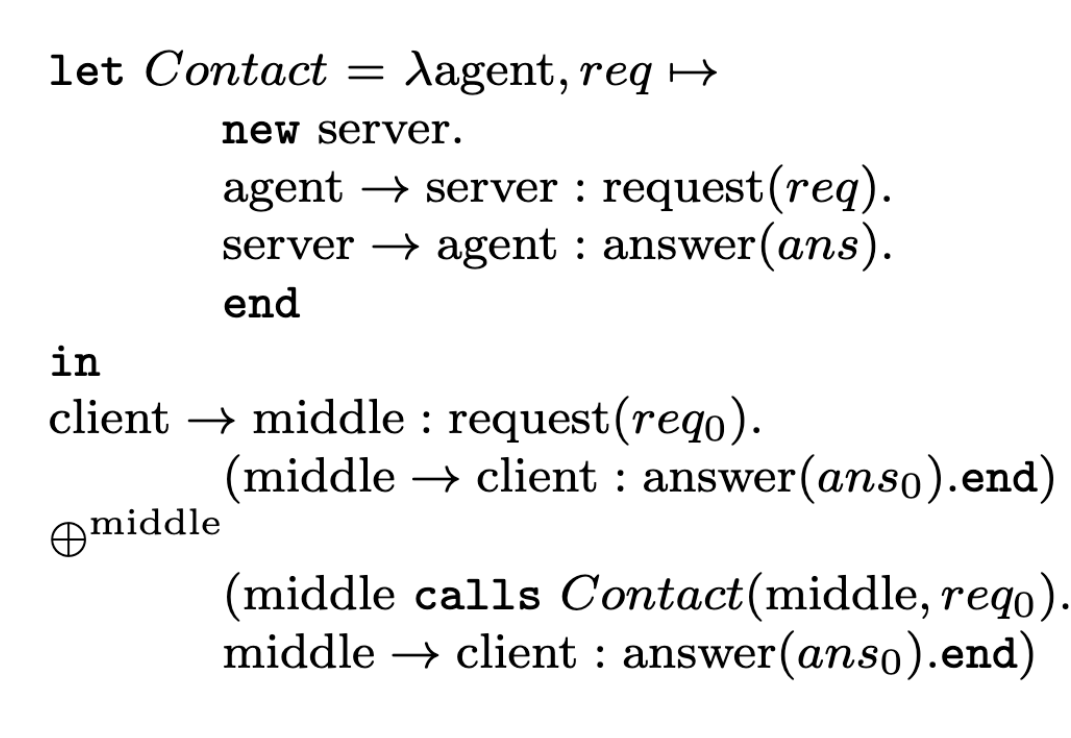
\includegraphics[scale=0.5]{nested_session_example.png}
    \caption{Example of Global Session Type for CPS Protocol\cite{nestedprotocols}\comment{nested protocols snippet}}
    \label{nested_session_example}
\end{figure}{}

% \subsection{Code Generation in Golang}
% Gois a popular industrial systems language.1One of its primary design features is first-classlanguage support for lightweight concurrency on multicore machines. Go offers easy spawningof parallel coroutines, calledgoroutines, that are transparently multiplexed over an underlyingset of system threads. Goroutines communicate and synchronize via message passing over typedchannels, designed to alleviate the difficulties of low-level mechanisms such as mutexes, conditionvariables and memory barriers commonly used in systems programming. As first-class objects, aninteresting andusefulfeature is the ability to passchannels over channels.Go is also well-established in distributed systems; e.g., it is the implementation language offrameworks such as Kubernetes, Docker and Jaeger. As the aforementioned concurrency features ofGo are specific to shared memory, a significant class of distributed programming in Go is conductedusing channel-based networking libraries via TCP, HTTP, etc. as transports. Developers appreciateGo since distributed programming in practice often involves local concurrency: goroutines andchannels are effective for dealing locally with the inherent asynchrony of distributed interactions
% For this project, the aim is to be able to generate a correct implementation of a protocol which uses nested protocols given a MPST-based specification. The target language for the framework to be developed is Go. Go is a popular programming language in industry. It has already been used to develop large projects like Docker and Kubernetes, and one of the reasons for its popularity is that it has inbuilt concurrency mechanisms. It has light-weight 

% In order for a global type to be well-formed, it must be projectable and well-kinded. Informally, well-kind which informally means that a mapping from all the identifiers in the global type to kinds can be found which 
%%%%%%%%%%%%%%%%%%%%%%%%%%%%%%%%%%%%

\chapter{Extending Scribble with Nested Protocols}\label{scribble-extensions-chapter}
% TODO: Verify this after extending Scribble background
In this chapter we extend the Featherweight Scribble language\cite{scribble} to model nested protocols. We extend the syntax of both global and local types with contructs for representing nested protocols similar to the ones described in \cite{nestedprotocols}. We introduce a precise definition of a protocol's scope - the protocols which are able to call a protocol, and extend the definition of well-formedness to take our syntax extensions into account. Finally, we extend the projection of Scribble global protocols with the new constructs we introduce.



\section{Syntax Extensions}\label{scribble-extensions}

% Scribble already allows defining multiple protocols in one module and protocols calling each other. However, in order to represent nested protocols, we need to extend Scribble with the ability to define protocols inside other protocols. Moreover, in the current implementation, protocol calls essentially correspond to inlining the interactions of the called protocol, but, as described in Section \ref{nested-session-types}, nested protocol calls involve inviting participating roles, external participants into the subsession and accepting the invitations before carrying out the interactions of the called protocol. Therefore, we will extend the Scribble syntax with suitable constructs for these operations and incorporate the semantics of nested protocol calls into the framework.\\

In Section \ref{Scribble} we described how the Scribble syntax already has most of the constructs needed to encode session types, including constructs for encoding labelled message exchanges, recursion and external choice. However, the session types pesented in the nested sessions paper\cite{nestedprotocols}, which we describe in Section \ref{nested-session-types}, also include some constructs which are not currently implemented in Scribble, like the internal choice session type. We have decided to focus on implementing the main functionality related to nested protocols, such as making it possible to declare protocols inside other protocols and introducing the use of invitations in order to participate in a nested protocol call, rather than extending Scribble with other non-essential constructs. We will therefore not support internal choice, but this should not be a great limitation, as the external choice construct will suffice for most use cases.
\\

In the definition of nested protocols presented in \cite{nestedprotocols}, which can be seen in Section \ref{nested-session-types}, a nested protocol call could also specify values which should be passed into the subsession. We will not support the ability to send values when calling a nested protocol explicitly. However, in the protocol implementation we will provide a means for the user to pass in values to subsessions by initialising the state of the different roles which will participate in the nested protocol, so this omission should not have a great impact in practice.\\

We introduce a precise definition for the scope of protocols, which the original paper\cite{nestedprotocols} did not handle explicitly. Through the use of scopes, the users can encapsulate different behaviours as nested protocols which can only be used inside a protocol, and these scope restrictions will be verified by the framework.\\

\subsection{Global Protocols}\label{scr-global-protocols}

We have extended the definition of a Scribble module, which we described in Section \ref{Scribble}, with nested protocols. Previously, a module was a collection of global protocols, but now it can also contain zero or more top-level nested protocols. However, it must still contain at least one global protocol (with no dynamic roles), which can be used as the entry point for the computation. As in \cite{nestedprotocols}, nested protocols can also be defined inside both nested and global protocols.\\

Although nested protocols could in theory be defined anywhere within a scope, for ease of parsing in the Scribble implementation and to provide more structured Scribble modules, we restrict the location where nested protocol can be declared. At the top-level, any nested protocols must be defined before the global protocol declarations, and within other protocols, they must be declared before any of the interactions. However, these restrictions do not impact the expressiveness of the implementation, as the order of the protocol declarations within a scope does not matter.\\

\begin{figure}[!h]
    \begin{center}
        \begin{tabular}{l}
            % \begin{math}
            %     \begin{array}{@{}rcl}
            %         \mathit{Module} & ::= & \mathit{N}\!*\ \mathit{P}+\\[7.5pt]
            %         \mathit{PBody} & ::= & \mathit{N}\!*\ \mathit{G}
            %     \end{array}
            % \end{math}\\[18pt]
            $\mathit{Module}\ ::=\ \mathit{N}\!*\ \mathit{P}+$\\[8pt]

            $\mathit{PBody}\ ::=\  \mathit{N}\!*\ \mathit{G}$\\[8pt]

            $\mathit{N}\ ::=\ \nested\ \protocol\ \mathit{pro}(\rolessig{A}{n};\ \scrnew\ \rolessig{B}{m})\ \{\;\mathit{PBody}\;\}$\\[8pt]
            
            \begin{math}
                \begin{array}{@{}rcl}
                    \mathit{P} & ::= & \scrglobal\ \protocol\ \mathit{pro}(\rolessig{A}{n})\ \{\;\mathit{PBody}\;\}\\[5pt]
                    \mathit{G} & ::= &\\[2.75pt]
                        &   | & \choice\ \at\ \mathit{A}\ \{\;\mathit{G_1}\;\}\ \scror\ ...\ \scror\ \{\;\mathit{G_n}\;\} \\[2.75pt]
                        &   | & \scrmessage{a}{S}\ \from\ \mathit{A}\ \scrto\ \mathit{B};\ \mathit{G} \\[2.75pt]
                        &   | & \rec\ \mathit{t}\ \{\;G\;\} \\[2.75pt]
                        &   | &  \continue\ \mathit{t} \\[2.75pt]
                        &   | & \scrdo\ \mathit{pro}(\roles{A}{n});\ \mathit{G} \\[2.75pt]
                        &   | &  \mathit{A}\ \calls\ \mathit{pro}(\roles{A}{n});\ G\\[2.75pt]
                        &   | & \scrend \\[2.75pt]
                \end{array}
            \end{math}
        \end{tabular}
    \end{center}
    % $\mathit{Module}\ ::=\ \mathit{N}\!*\ \mathit{P}+$\\[8pt]

    % $\mathit{PBody}\ ::=\  \mathit{N}\!*\ \mathit{G}$\\[8pt]

    % $\mathit{N}\ ::=\ \nested\ \protocol\ \mathit{pro}(\rolessig{A}{n};\ \scrnew\ \rolessig{B}{m})\ \{\;\mathit{PBody}\;\}$\\[8pt]

    % $\mathit{P}\ ::=\ \scrglobal\ \protocol\ \mathit{pro}(\rolessig{A}{n})\ \{\;\mathit{PBody}\;\}$\\[8pt]

    % \begin{center}$
    %     \begin{array}{rcl}
    %         \mathit{G} & ::= &\\[2.75pt]
    %             &   | & \choice\ \at\ \mathit{A}\ \{\;\mathit{G_1}\;\}\ \scror\ ...\ \scror\ \{\;\mathit{G_n}\;\} \\[2.75pt]
    %             &   | & \scrmessage{a}{S}\ \from\ \mathit{A}\ \scrto\ \mathit{B};\ \mathit{G} \\[2.75pt]
    %             &   | & \rec\ \mathit{t}\ \{\;G\;\} \\[2.75pt]
    %             &   | &  \continue\ \mathit{t} \\[2.75pt]
    %             &   | & \scrdo\ \mathit{pro}(\roles{A}{n});\ \mathit{G} \\[2.75pt]
    %             &   | &  \mathit{A}\ \calls\ \mathit{pro}(\roles{A}{n});\ G\\[2.75pt]
    %             &   | & \scrend \\[2.75pt]
    %     \end{array}
    % $\end{center}
    % }
    \caption{Syntax for Scribble module with nested protocols}
    \label{scribble-nested-syntax-global}
\end{figure}

% \begin{figure}[!h]
%     \begin{itemize}
%         \item $\mathit{Module}\ ::=\ \mathit{N}\!*\ \mathit{P}+$
%         \item $\mathit{N}\ ::=\ \nested\ \protocol\ \mathit{pro}(\rolessig{A}{n};\ \scrnew\ \rolessig{B}{m})\ \{\;\mathit{PBody}\;\}$
%         \item  $\mathit{P}\ ::=\ \scrglobal\ \protocol\ \mathit{pro}(\rolessig{A}{n})\ \{\;\mathit{PBody}\;\}$
%         \item $\mathit{PBody}\ ::=\  \mathit{N}\!*\ \mathit{G}$
%         \item $\mathit{G}\ ::= $
        
%         $\quad\quad|\ \choice\ \at\ \mathit{A}\ \{\;\mathit{G_1}\;\}\ \scror\ ...\ \scror\ \{\;\mathit{G_n}\;\}$
    
%         $\quad\quad|\ \scrmessage{a}{S}\ \from\ \mathit{A}\ \scrto\ \mathit{B};\ \mathit{G}$
        
%         $\quad\quad|\ \rec\ \mathit{t}\ \{\,\mathit{G}\;\}$
        
%         $\quad\quad|\ \continue\ \mathit{t}$
        
%         $\quad\quad|\ \scrdo\ \mathit{pro}(\roles{A}{n});\ G$
    
%         $\quad\quad|\ \mathit{A}\ \calls\ \mathit{pro}(\roles{A}{n});\ G$
        
%         $\quad\quad|\ \scrend$
    
%     \end{itemize}
%     \caption{Syntax for Scribble module with nested protocols}
%     \label{scribble-nested-syntax-global}
% \end{figure}


A formal specification of our proposed syntax for Scribble modules with nested protocols is given in Figure \ref{scribble-nested-syntax-global}, and we provide some examples of global and nested protocols in Figure \ref{scribble-nested-global}. We introduce several new keywords in order to define nested protocols and calls to nested protocols, while trying to preserve as much of the original syntax and behaviour as possible.
\begin{itemize}
    \item The $\nested$ keyword can be used to define protocols with dynamic participants. Dynamic participants are separated from regular participants by a $\scrnew$ keyword in the protocol declaration. However, nested protocols need not have dynamic participants, in which case the latter part of the declaration can be omitted. When a protocol is defined within another protocol, it restricts the scope where it can be used, much like defining a nested function in a programming language. We also support shadowing of protocol names: if you redefine a protocol in an inner scope, then it will override the previous definition in that scope and all its subscopes.
    \item The $\calls$ construct introduces a subsession, where a role calls a nested protocol, inviting a set of roles to carry out the interactions of the nested protocol. In a $\calls$ construct the dynamic participants of the nested protocol are omitted - it is only necessary to specify which existing roles which be participating, as the remaining roles will be dynamically created.
    \item We modify the semantics of the $\scrdo$ construct, which previously resulted in expanding the interactions of the called protocol, to instead create a subsession. Its semantics are equivalent to a $\calls$ construct, where the first partipant in the protocol is treated as the caller. However, we restrict the use of the $\calls$ construct to only call nested protocols and the $\scrdo$ construct to call global protocols. 
    \item The distinction between global and nested protocols is important, and needs to be verified to ensure that any protocol call used the correct construct. Moreover, protocol calls need to be verified to ensure that the call matches the signature of the protocol which is in scope, as protocol declarations with the same protocol name in different scopes may involve a different number of participants.
    \item As we did in Section \ref{Scribble}, we simplify the notation for labelled messages. Even though we only write down labelled messages with one payload field, Scribble also supports user-defined labelled messages with zero or more payload fields. In our implementation the user may optionally define names for any of the payload fields as well. However, there cannot be any duplicate field names within a message.
    \item As before, the $\scrend$ construct can be omitted when writing down protocol declarations.
\end{itemize}

\begin{figure}[h]
    \centering
    \lstset{language=Scribble}
    \begin{lstlisting}
    
    nested protocol NestedProtocol(role X; new role Y) {
        do GlobalProtocol(X, Y);
    }
    
    global protocol GlobalProtocol(role A, role B) {
        B calls NestedProtocol(A);
    }
        \end{lstlisting}
        \caption{Scribble syntax for nested protocols}
        \label{scribble-nested-global}
    \end{figure}{}
 
\subsection{Scopes}

As it was briefly mentioned in Section \ref{scribble-extensions}, the definition of nested protocols presented in \cite{nestedprotocols} did not handle the scopes in which protocols could be called explicitly. In our Scribble extension we provide a more precise definition of protocol's scope and how it affects which protocols can be called from within different protocols in a Scribble module.\\

In a Scribble module we have the top-level scope, where the user can define global and nested protocols which can be called from any protocol, no matter how deeply nested its declaration is. As we mentioned in Section \ref{scr-global-protocols}, each protocol declaration introduces a new scope of its own.  Any nested protocols defined within are not visible outside that  protocol, but can be used in that protocol's implementation and any nested protocols defined within.\\

The main restriction we have applied is that within any given scope, there must never be a clash between protocols of the same kind. For simplicity, the naming conflicts only take into account the name of the protocol rather than the full signature. This means that global protocols, which can only be defined at the top level, must always have unique names, and no two nested protocols defined in the same scope can have the same name.

\subsubsection{Global vs Nested Protocols}

The distinction between the $\scrdo$ and $\calls$ constructs for calling global and nested protocols makes it possible to unambiguously define a nested protocol and a global protocol with the same name without one definition shadowing the other. However, in this case the user must be careful when calling the protocol, especially if they have signatures with the same number of non-dynamic participants, as it can be easy to confuse which protocol call was intended. If the signatures are different this should be less of a problem, as trying to call a protocol with the wrong number of participants will produce an error.\\

As we mentioned in Section \ref{scr-global-protocols}, defining a nested protocol with the same name as a nested protocol in an outer scope will override the definition in the current scope and any inner scopes. Global protocol definitions cannot be shadowed, as they can only be defined within the top-level scope. When checking that protocol calls are valid it is is important to keep track of the protocols which are currently in scope and their signatures to ensure that the call matches the number of roles in the protocol's signature. 

\subsection{Local Protocols}

After extending the syntax for Scribble global protocols we also had to modify the definition of projection of Scribble global types presented in \cite{featherweight} to include these new constructs, which we describe in Section \ref{scribble-projection}. We therefore extend the syntax of Scribble local types with constructs for sending and receiving invitations following the session types presented in \cite{nestedprotocols}. \\

% \begin{figure}[h!]
%     \begin{itemize}
%         \item $L ::=\scrlocal\ \protocol\ A@pro(\role A_1,\ ...,\ \role A_n;\ \scrnew\ \role\ B_1,\ ...,\ \role\ B_m)\ \{T\}$
%         \item $T ::= $
        
%         $\quad\quad|\ \choice\ \at\ A\ \{T_1\}\ \scror\ ...\ \scror\ \{T_n\}$
    
%         $\quad\quad|\ \scrmessage{a}{S}\ \from\ B;\ T$
    
%         $\quad\quad|\ \scrmessage{a}{S}\ \scrto\ B;\ T$
        
%         $\quad\quad|\ \rec\ t\ \{T\}$
        
%         $\quad\quad|\ \continue\ t$
        
%         $\quad\quad|\ \invite(A_1,\ ...\ ,\ A_n)\ \scrto\ pro;\ T$
        
%         $\quad\quad|\ \create(\role\ B_1,\ ...\ ,\role\ B_n)\ \scrin\ pro;\ T$
    
%         $\quad\quad|\ \accept\ C@pro(A_1,\ ...\ ,\ A_n;\ \scrnew\ B_1,\ ...\ ,\ B_m)\ \from\ A;\ T$
    
%         $\quad\quad|\ \scrend$
%     \end{itemize}
%     \caption{Syntax of Scribble local protocols extended with invitations}
%     \label{scr-local-protocols-syntax}
% \end{figure}

\begin{figure}[h!]
    \begin{center}
        \begin{tabular}{l}
            $\mathit{L}\ ::=\ \scrlocal\ \protocol\ \mathit{A@pro}(\rolessig{A}{n};\ \scrnew\ \rolessig{B}{m})\ \{\;T\;\}$ \\\\
            \begin{math}
                \begin{array}{@{}rcl}
                    \mathit{RecvMsg} & ::= & \\[2.75pt]
                     & | & \messageFromL{a}{S}{B}\,;\\[2.75pt]
                     & | & \acceptL{C@pro}{A}{B}{A}\,;\\\\
        
                    \mathit{T} & ::= &\\[2.75pt]
                      &   | & \choice\ \at\ \mathit{A}\ \{T_1\}\ \scror\ ...\ \scror\ \{T_n\} \\[2.75pt]
                      &   | & \rec\ \mathit{t}\ \{\;T\;\} \\[2.75pt]
                      &   | &  \continue\ \mathit{t} \\[2.75pt]
                      &   | & \scrmessage{a}{S}\ \scrto\ \mathit{B};\ \mathit{T} \\[2.75pt]
                    %   &   | & \scrmessage{a}{S}\ \from\ \mathit{B};\ \mathit{T} \\[2.75pt]
                      &   | & \mathit{RecvMsg}\ \mathit{T}\\[2.75pt]
                      &   | & \invite(\roles{A}{n})\ \scrto\ \mathit{pro}\,;\ \mathit{T} \\[2.75pt]
                      &   | & \create(\rolessig{B}{m})\ \scrin\ \mathit{pro}\,;\ \mathit{T}\\[2.75pt]
                    %   &   | & \accept\ \mathit{C@pro}(\roles{A}{n};\ \scrnew\ \roles{B}{m})\ \from\ \mathit{A}\,;\ \mathit{T}\\[2.75pt]
                    &   | & \scrend \\[2.75pt]
                \end{array}
            \end{math}
        \end{tabular}
    \end{center}
    \caption{Syntax of Scribble local protocols extended with invitations}
    \label{scr-local-protocols-syntax}
\end{figure}

% \begin{figure}[h!]
%     \centering
%     \begin{math}
%         \begin{array}{rcl}
%             \mathit{L} & ::= & \scrlocal\ \protocol\ \mathit{A@pro}(\rolessig{A}{n};\ \scrnew\ \rolessig{B}{m})\ \{\;T\;\} \\\\
%             % G & ::= & \texttt{end} & \white &
            
%             \mathit{RecvMsg} & ::= & \\[2.75pt]
%              & | & \messageFromL{a}{S}{B}\\[2.75pt]
%              & | & \acceptL{C@pro}{A}{B}{A}\\\\

%             \mathit{T} & ::= &\\[2.75pt]
%               &   | & \choice\ \at\ \mathit{A}\ \{T_1\}\ \scror\ ...\ \scror\ \{T_n\} \\[2.75pt]
%               &   | & \scrmessage{a}{S}\ \from\ \mathit{B};\ \mathit{T} \\[2.75pt]
%               &   | & \scrmessage{a}{S}\ \scrto\ \mathit{B};\ \mathit{T} \\[2.75pt]
%               &   | & \rec\ \mathit{t}\ \{\;T\;\} \\[2.75pt]
%               &   | &  \continue\ \mathit{t} \\[2.75pt]
%               &   | & \invite(\roles{A}{n})\ \scrto\ \mathit{pro}\,;\ \mathit{T} \\[2.75pt]
%               &   | & \create(\rolessig{B}{m})\ \scrin\ \mathit{pro}\,;\ \mathit{T}\\[2.75pt]
%               &   | & \accept\ \mathit{C@pro}(\roles{A}{n};\ \scrnew\ \roles{B}{m})\ \from\ \mathit{A}\,;\ \mathit{T}\\[2.75pt]
%               &   | & \scrend \\[2.75pt]
%         \end{array}
%     \end{math}
%     \caption{Syntax of Scribble local protocols extended with invitations}
%     \label{scr-local-protocols-syntax}
% \end{figure}

Our proposed extensions to the syntax of Scribble local protocols are shown in Figure \ref{scr-local-protocols-syntax}, and some examples of local protocols, which correspond to the projections of the protocols in Figure \ref{scribble-nested-global}, are can be seen in Figure \ref{scribble-nested-local}. We have kept all the original Scribble constructs and added three new ones for sending invitations, accepting invitations and for initializing dynamic roles:

\begin{itemize}
    \item The sending of internal invitations is expressed by the $\invite$ construct, which specifies the roles which are going to participate, and the name of the protocol to which they are invited. The syntax for the $\invite$ contruct shown above can be seen as a shorthand for sending a series of individual invitations in parallel (asynchronously) to all the roles who are going to participate in the protocol. Indeed, this idea could be expressed with an alternative notation such as:
    $\{\invite(A_i)\ \scrto\ pro;\}_{i \in \{1,\ ...\ ,\ n\}};\ T$

    \item Bringing new participants into the subsession through external invitations is done through the $\create$ statement, which specifies the dynamic roles of the protocol to be created. Similarly to the $\invite$ construct, the proposed syntax can be seen as a shorthand for the sending in parallel of external invitations.
    
    \item Internal invitations are accepted through the $\accept$ construct, which contains information about the participant which sent the inviation, the local protocol which the role is going to be carrying out as well as all the other roles which will be participating as well.
\end{itemize}

% TODO: verify projection
\begin{figure}[htb!]
    \centering
    \lstset{language=Scribble}
    \begin{lstlisting}
    
    local protocol X@NestedProtocol(role X; new role Y) {
        invite(X, Y) to GlobalProtocol;
        accept A@GlobalProtocol(X, Y);
    }

    local protocol Y@NestedProtocol(role X; new role Y) {
        accept B@GlobalProtocol(X, Y);
    }
    
    local protocol A@GlobalProtocol(role A, role B) {
        accept X@NestedProtocol(A; new Y) from B;
    }

    local protocol B@GlobalProtocol(role A, role B) {
        invite(A) to NestedProtocol;
        create(role Y) in NestedProtocol;
    }
    \end{lstlisting}
    \caption{Scribble syntax for nested protocols}
    \label{scribble-nested-local}
\end{figure}{}

\section{Well-formedness}
% When moving this, I need to ensure that I define what a valid protocol call is before it is refered to in other places.
In order to be able to generate the implementation of a protocol specified by the user, the Scribble framework must first verify that the protocol is well-formed.\\ According to the definitions in \cite{featherweight, nestedprotocols}, in order for a protocol to be well-formed it must be projectable and all protocol calls must be valid. A protocol is projectable if the projection is defined for all the participants of that protocol, and a protocol call is valid if the called protocol is defined/in scope, it is called with the correct number of roles and all the roles involved are distinct and in scope (participating in the current protocol).\\

Despite our extensions to the Scribble framework, the well-formedness property remains the same. However, we highlight the importance of ensuring that protocol calls are valid after introducing nested scopes and the ability to shadow protocol declarations, which makes it possible users to declare protocols with the same name and different declarations in different scopes. We also extend the definition of projection given in \cite{nestedprotocols} by incorporating the full merge operator, which the original paper did not. In order to do this, we extend the definition of the merge operator defined in \cite{featherweight}.

% The well-formedness property for protocols still remains the same as before \cite{nestedprotocols}\cite{featherweight}. We say a protocol is well-formed if it is projectable and all protocol calls are valid. A protocol is projectable if the projection is defined for all the participants of that protocol. We incorporate the merging operator into the projection, which the original paper did not, extending the definition with the cases for invitations. A protocol call is valid if the protocol called is in scope, it is called with the correct number of roles and all the roles involved are distinct and in scope (participating in the current protocol).

\section{Renaming Protocols}\label{renaming}

The representation of Scribble nested protocols we have defined in Section \ref{scr-global-protocols} is similar to the representation of nested protocols given in \cite{nestedprotocols}. However, the distinction between global and nested protocols and protocol calls in Scribble makes it more complicated and verbose to define the projection of protocols, and name clashes between protocols in different scopes will need to be resolved at some point before code generation to be able to generate a correct implementation of the protocols.\\

In order to simplify the process, we propose introducing an extra preprocessing step on the protocols before projecting them, once the global and nested protocols have been validated to ensure they are syntactically correct and that all protocol calls are valid. The objective in this step is to generate a simpler, flattened representation of the Scribble module, where all the protocols are stored in a single set. In order to achieve this, name clashes need to be resolved to ensure that all protocol names are unique, and all references to the protocols in protocol calls must be renamed to the new unique names. Ensuring that all protocol names are globally unique has the added advantage of enabling us to remove the distinction between nested and global protocols and treat protocol calls to both global and nested protocols uniformly, as there can be no ambiguity with regards to which protocol is going to be called.\\

The result of this renaming process is a set of protocols which do not contain any nested protocols within, where both global and nested protocols have been converted into this intermediate representation. We define a different syntax for this representation, as shown in Figure \ref{protocols-after-renaming}, which is essentially the same as a nested protocol declaration without any nested protocols inside.\\

\begin{figure}[h!]
    \centering
    $\protocol\ P(\role\ A_1,\ ...,\ \role\ A_n;\ \scrnew\ \role\ B_1,\ ...,\ \role\ B_m)\ \{\;G\;\}$\\
    \caption{Intermediate representation of protocols after renaming}
    \label{protocols-after-renaming}
\end{figure}

We present a renaming algorithm which uses two environments. The first one maps the original protocol names that were accessible in the current scope to the unique names of the protocols they refer to, while the second environment holds the set of all the unique protocol names which have been generated. The scope environment can be used to update the protocol calls in the interactions of a protocol, and the protocol name environment is necessary to generate globally unique protocol names. We define the algorithm in pseudocode in Figures \ref{renaming-interactions} and \ref{renaming-module}.

\subsection{Renaming Protocol Declarations}

The first step in the algorithm is to aggregate the information from the protocol declarations in the \textbf{top-level scope} into both environments. When resolving clashes between top-level nested and global protocols we decided to always change the nested protocol names and keep the global protocol names without changing them. With this approach we are able to only keep a single environment for the nested protocols which are in the current scope, as global protocol names will not change, so there is no need to track them in a separate environment. We add the unique names of both the top-level global and nested protocols to the protocol name environment, and store a mapping from the nested protocol names to their new unique names in the scope environment. As well as updating the environments, we also change the protocol names in the nested protocol declarations. This process can be seen in lines 15-25 of the \texttt{rename\_module} function in Figure \ref{renaming-module}.\\

Once we have all the information about the top-level scope, we can proceed to \textbf{recursively rename} the interactions of all the protocols, aggregating all the resulting protocols in a single set. In order to update the interactions of a protocol, we must first update both the scope and protocol name environments with the nested protocol declarations inside the current protocol. The procedure for how this can be done is shown in the function \texttt{rename\_nested\_protocols} in Figure \ref{renaming-interactions}. We first generate a new unique name for each of the protocols and add it to the protocol name environment. The scope environment is updated by creating/modifying the mapping for the protocol's old name so that it refers to the new name. We also update the declarations of the nested protocols with their new unique names here. Once both environments have been updated, we recursively rename the interactions of each of the nested protocols and store them in the result set. Finally, we update the protocol names in the current protocol's interactions using the scope environment and add the protocol with its new interactions to the result set.
 
\subsection{Renaming Protocol Interactions}

The procedure we have just described is implemented in the \texttt{\seqsplit{rename\_and\_flatten\_protocols}} function in Figure \ref{renaming-module}. We need to return the updated protocol name environment as well as the set of renamed protocols to ensure that the protocol names we generate are unique. Otherwise, clashes could occur between protocols defined inside different nested protocols. However, the scope environment does not contain any useful information outside the current scope, so it can be ignored once the protocol's interactions have been updated. \\

Renaming a protocol's interactions simply requires recursively traversing the global type, as shown in the \texttt{rename\_protocol\_calls} function in Figure \ref{renaming-interactions}. The only interactions which change are the global protocol calls and nested protocol calls. In order to treat both types of calls in the same way, global protocol calls are converted explicitly to the $\calls$ construct with the first participant initiating the call. As global protocol names were not changed, the protocol name in the call remains the same. On the other hand, updating nested protocol calls requires looking up the unique protocol name corresponding to the protocol being called in the scope environment and building a new $\calls$ construct with it.\\

\begin{figure}[h!]
    \centering
    \lstset{language=Pseudocode}
    \begin{lstlisting}[escapeinside={(*}{*)}]
    def rename_protocol_calls(G, ScopeEnv):
        match G with:
            | A calls P((*$\roles{A}{n}$*)); (*$\mathtt{G_1}$*) ->
                newP = ScopeEnv[P]
                (*new$\mathtt{G_1}$*) = rename_protocol_calls((*$\mathtt{G_1}$*), ScopeEnv)
                return A calls newP((*$\roles{A}{n}$*)); (*new$\mathtt{G_1}$*)
            | do P((*$\roles{A}{n}$*)); (*$\mathtt{G_1}$*) -> 
                (*new$\mathtt{G_1}$*) = rename_protocol_calls((*$\mathtt{G_1}$*), ScopeEnv)
                return (*$\mathtt{A_1}$*) calls P((*$\roles{A}{n}$*)); (*new$\mathtt{G_1}$*)
            | choice at A (*$\mathtt{\{\;G_i\,\}_\varinset{i}{I}}$*) ->
                return choice at A (*$\mathtt{\{\;\;rename\_protocol\_calls(G_i,\ ScopeEnv)\;\;\}_\varinset{i}{I}}$*)
            | rec t (*$\mathtt{\{\;G_1\,\}}$*) -> 
                (*new$\mathtt{G_1}$*) = rename_protocol_calls((*$\mathtt{G_1}$*), ScopeEnv)
                return rec t (*$\mathtt{\{\;newG_1\,\}}$*)
            | a(S) from A to B; (*$\mathtt{G_1}$*) ->
                (*new$\mathtt{G_1}$*) = rename_protocol_calls((*$\mathtt{G_1}$*), ScopeEnv)
                return a(S) from A to B; (*new$\mathtt{G_1}$*)
            | continue t ->
                return continue t
            | end ->
                return end
        
    def rename_nested_protocols(nested_protocols, ScopeEnv, ProtocolNames):
        renamed_protocols = (*$\emptyset$*)
        for (nested protocol P((*$\rolessig{A}{n}$*); (*$\scrnew\ \rolessig{B}{m}$*)) {nested_protos; G}) in nested_protocols:
            newP = UNIQUE_NAME(P, ProtocolNames)
            ScopeEnv = ScopeEnv[P -> newP]
            ProtocolNames = ProtocolNames (*$\bigcup$*) {newP}
            renamed_protocols = renamed_protocols (*$\bigcup$*) {(*$\;$*)nested protocol newP((*$\rolessig{A}{n}$*); (*$\scrnew\ \rolessig{B}{m}$*)) {nested_protos; G}(*$\;$*)}
        return (renamed_protocols, ScopeEnv, ProtocolNames)
    \end{lstlisting}
    \caption{Algorithm for renaming protocol interactions}
    \label{renaming-interactions}
\end{figure}
\clearpage

\begin{figure}[h!]
    \centering
    \lstset{language=Pseudocode}
    \begin{lstlisting}[escapeinside={(*}{*)}]
    def rename_and_flatten_protocols(nestedProtocol, ScopeEnv, ProtocolNames, AllProtocols):
        match nestedProtocol with:
          | nested protocol P((*$\rolessig{A}{n}$*); new (*$\rolessig{B}{m}$*)) {nested_protocols; G} ->
            (ScopeEnv, ProtocolNames, nestedProtocols) = 
                rename_nested_protocols(nestedProtocols, ScopeEnv, ProtocolNames)
            for nestedProtocol in nestedProtocols:
              ProtocolNames, AllProtocols = 
                  rename_and_flatten_protocols(nestedProtocol, ScopeEnv, ProtocolNames, AllProtocols)

            newG = rename_protocol_calls(G, ScopeEnv)
            AllProtocols = AllProtocols (*$\bigcup$*) {(*$\;$*)protocol P((*$\rolessig{A}{n}$*); new (*$\rolessig{B}{m}$*)) {(*$\;$*)newG(*$\;$*)}(*$\;$*)}
            return ProtocolNames, AllProtocols
      
    def rename_module(nested_protocols, global_protocols):
        ProtocolNames = (*$\emptyset$*)
        ScopeEnv = {}
        TopLevelProtocols = (*$\emptyset$*)
        AllProtocols = (*$\emptyset$*)
        for (global protocol P((*$\rolessig{A}{n}$*)) {nested_protos; G}) in global_protocols:
          ProtocolNames = ProtocolNames (*$\bigcup$*) P
          TopLevelProtocols = TopLevelProtocols (*$\bigcup$*) {nested protocol P((*$\rolessig{A}{n}$*); (*$\emptyset$*)) {nested_protos; G}}

        renamed_nested_protocols, ScopeEnv, ProtocolNames = 
              rename_nested_protocols(nested_protocols, ScopeEnv, ProtocolNames)
        TopLevelProtocols = TopLevelProtocols (*$\bigcup$*) renamed_nested_protocols
        for top_level_protocol in TopLevelProtocols:
            ProtocolNames, AllProtocols = rename_and_flatten_protocols(top_level_protocol, SetupEnv, ProtocolNames, AllProtocols)

        return AllProtocols

    \end{lstlisting}
    \caption{Algorithm for renaming protocols in a Scribble module}
    \label{renaming-module}
\end{figure}
\clearpage


\section{Projection}\label{scribble-projection}
Like definition of projection presented in \cite{nestedprotocols}, projecting a global or nested protocol requires having an environment which keeps track of all the protocols which are in scope. Our definition of projection is defined on the flattened representation of the Scribble module we described in Section \ref{renaming}, where all the protocols are stored in one large set and the distinction between global and nested protocols has been removed. Moreover, in order to successfully rename all the protocols the original Scribble module must have been checked to ensure all protocol calls are valid. From this flattened representation, building the projection environment is a trivial process, where the protocol declarations in the set can be aggregated to create a mapping from protocol names to their role signatures ($P \mapsto \{\roles{A}{n};\ \roles{B}{m}\}$).\\

It is not a problem to store the signatures of all the protocols in the environment, because in the validation step and the renaming process we will have already verified that the scope restriction is not violated, so the protocols will only ever need to look up protocols which are defined in their scope in the projection environment. The definition of projection is undefined for protocol calls to protocols which are not in the environment, but this case should never arise if the protocols have passed the previous validation steps we have described.

\subsection{Projection of Global Protocols}

In order to generate all the local protocols in a Scribble module, we must project every protocol onto every role taking part in it, which will generate a much larger set of local protocols. We define the projection of a Scribble protocol $P$ onto a role $A$ in Figure \ref{scribble-protocol-projection}.

\begin{figure}[!h]
    \begin{center}
        \begin{tabular}{l}
            $(\protocol\ \mathit{P}(\rolessig{A}{n};\ \scrnew\ \rolessig{B}{m})\ \{\mathit{G}\})\project\ =$\\[7pt]
            \begin{math}
                \begin{cases}
                    \mathit{If}\ \mathit{A} \in \{\roles{A}{n},\ \roles{B}{m}\}:\\
                    \scrlocal\ \protocol\ \mathit{A@P}(\rolessig{A}{n};\ \scrnew\ \rolessig{B}{m})\ \{\mathit{G} \project\}\\[8pt]
                    \mathit{Otherwise:} \quad \mathit{undefined}
                \end{cases}
            \end{math}
        \end{tabular}
    \end{center}
    \caption{Projection of a Scribble protocol}
    \label{scribble-protocol-projection}
\end{figure}
% If $A \in \{\roles{A}{n},\ \roles{B}{m}\}$ then:

% $(\protocol\ P(\rolessig{A}{n};\ \scrnew\ \rolessig{B}{m})\ \{G\})\downarrow_A^{Env}\ =$

% $\scrlocal\ \protocol\ A@P(\rolessig{A}{n};\ \scrnew\ \rolessig{B}{m})\ \{G \downarrow_A^{Env}\}$\\

% Otherwise it is undefined. \\


The projection operation on global protocols remains the same as defined in \cite{featherweight} for all constructs except the $\choice$. Figure \ref{featherweight-scribble-projections} shows these definitions, which we have taken from the paper. We denote $\mathcal{P}(G)$ as the set of roles participating in protocol $G$.\\

Previously, the $\scrdo$ construct would be expanded before projection, which we do not do. However, after removing the distinction between global and nested protocols, all calls to global protocols using the $\scrdo$ construct will have been converted to $\calls$, so we also do not need to define a rule for projecting $\scrdo$. 

\begin{figure}[!h]
    \begin{center}
        \begin{tabular}{l}
            $(\scrmessage{a}{S}\ \from\ \mathit{B}\ \scrto\ \mathit{C};\ G') \project\ =\ $\\[3.5pt]
            \begin{math}
                \begin{cases}
                    \scrmessage{a}{S}\ \scrto\ \mathit{C};\ (\mathit{G'} \project) & \mathit{if}\ \mathit{A}\ =\ \mathit{B}\\[3pt]
                    \scrmessage{a}{S}\ \from\ \mathit{B};\ (\mathit{G'} \project) & \mathit{if}\ \mathit{A}\ =\ \mathit{C}\\[3pt]
                    \mathit{G'} \project & \mathit{otherwise}
                \end{cases}
            \end{math}
            \\\\
            $(\rec\ \mathit{t}\ \{\mathit{G'}\}) \project\ =$\\[3.5pt]
            \begin{math}
               \begin{cases}
                   \rec\ \mathit{t}\ \{\mathit{G'} \project\} & \mathit{if}\ \mathit{A}\ \in\ \mathcal{P}(G')\\
                   \scrend & \mathit{otherwise}
               \end{cases}
           \end{math}
           \\\\
           $(\continue\ \mathit{t}) \project\ =\ \continue\ \mathit{t}$
           \\\\
           $(\scrend) \project\ =\ \scrend$
        \end{tabular}
    \end{center}
 
    \caption{Projection of constructs taken from Featherweight Scribble\cite{featherweight}}
    \label{featherweight-scribble-projections}
\end{figure}

\subsubsection{Projection of Protocol Calls}

The projection of the $\calls$ construct is based on the projection of the protocol call which was defined in \cite{nestedprotocols}, and it considers the same 4 cases. When the projected role is making a call, it must send all the invitations to the other participants, potentially including itself. It must also send external invitations to the new dynamic participants which will take part in the subsession, if any. If there are no dynamic participants, then the $\create$ construct can be omitted. If the projected role is taking part in the subsession, then it must also accept the invitation to the appropriate role in the nested protocol from the caller. If the projected role is neither the caller or a participant in the protocol call, then the protocol call can be ignored. The formal definition of the projection of the $\calls$ construct is shown in Figure \ref{scribble-calls-projection}\\
 
%  $(\scrmessage{a}{S}\ \from\ B\ \scrto\ C;\ G') \project\ =\ $\\[3.5pt]
% \begin{math}
%     \begin{cases}
%         \scrmessage{a}{S}\ \scrto\ C;\ (G' \project) & if\ A\ =\ B\\[3pt]
%         \scrmessage{a}{S}\ \from\ B;\ (G' \project) & if\ A\ =\ C\\[3pt]
%         G' \project & otherwise
%     \end{cases}\\\\
% \end{math}
 
%  $(\rec\ t\ \{G'\}) \project\ =$\\[3.5pt]
%  \begin{math}
%     \begin{cases}
%         \rec\ t\ \{G' \project\} & if\ A\ \in\ \mathcal{P}(G')\\
%         \scrend & otherwise
%     \end{cases}\\\\
% \end{math}
 
%  $(\continue\ t) \project\ =\ \continue\ t$\\
 
%  $(\scrend) \project\ =\ \scrend$\\
 
\begin{figure}[!h]
    \begin{center}
        \begin{tabular}{l}
            $(C\ \calls\ P(\roles{A}{n});\ G') \projectenv{Env,\ P\ \mapsto\ \{\roles{D}{n};\ \roles{B}{m}\}}\ =$\\[3.5pt]
            \begin{math}
                \begin{cases}
                    \invite(\roles{A}{n})\ \scrto\ \mathit{P}; & \mathit{if}\ \mathit{A}\ =\ \mathit{C},\ \exists i. \mathit{C}\ =\ \mathit{A_i}\\[0.25pt]
                    \create(\rolessig{B}{m})\ \scrin\ \mathit{P}; & \\[0.25pt]
                    \accept\ \mathit{D_i@P}(\roles{A}{n};\ \scrnew\ \roles{B}{m})\ \from\ \mathit{C}; & \\[0.25pt]
                    (\mathit{G'} \projectenv{Env,\ P\ \mapsto\ \{\roles{D}{n};\ \roles{B}{m}\}}) & \\[13pt]

                    \invite(\roles{A}{n})\ \scrto\ \mathit{P}; & \mathit{if}\ \mathit{A}\ =\ \mathit{C},\ \mathit{C} \notin \{\roles{A}{n}\} \\[0.25pt]
                    \create(\rolessig{B}{m})\ \scrin\ \mathit{P}; &\\[0.25pt]
                    (\mathit{G'} \projectenv{Env,\ P\ \mapsto\ \{\roles{D}{n};\ \roles{B}{m}\}}) &\\[13pt]

                    \accept\ \mathit{D_i@P}(\roles{A}{n};\ \scrnew\ \roles{B}{m})\ \from\ C; & \mathit{if}\ \mathit{A}\ \neq\ \mathit{C},\ \exists i. C\ =\ A_i\\[0.25pt]
                    (\mathit{G'} \projectenv{Env,\ P\ \mapsto\ \{\roles{D}{n};\ \roles{B}{m}\}}) & \\[13pt]

                    (\mathit{G'} \projectenv{Env,\ \mathit{P}\ \mapsto\ \{\roles{D}{n};\ \roles{B}{m}\}}) & \mathit{otherwise}
                \end{cases}
            \end{math}
        \end{tabular}
    \end{center}
    \caption{Projection of $\calls$ construct}
    \label{scribble-calls-projection}
\end{figure}

%  $(C\ \calls\ P(\roles{A}{n});\ G') \projectenv{Env,\ P\ \mapsto\ \{\roles{D}{n};\ \roles{B}{m}\}}\ =$\\[3.5pt]
%  \begin{math}
%     \begin{cases}
%         \invite(\roles{A}{n})\ \scrto\ P; & if\ A\ =\ C,\ \exists i. C\ =\ A_i\\[0.25pt]
%         \create(\rolessig{B}{m})\ \scrin\ P; & \\[0.25pt]
%         \accept\ D_i@P(\roles{A}{n};\ \scrnew\ \roles{B}{m})\ \from\ C; & \\[0.25pt]
%         (G' \projectenv{Env,\ P\ \mapsto\ \{\roles{D}{n};\ \roles{B}{m}\}}) & \\[13pt]

%         \invite(\roles{A}{n})\ \scrto\ P; & if\ A\ =\ C,\ C \notin \{A_1,\ ...\ ,\ A_n\} \\[0.25pt]
%         \create(\rolessig{B}{m})\ \scrin\ P; &\\[0.25pt]
%         (G' \projectenv{Env,\ P\ \mapsto\ \{\roles{D}{n};\ \roles{B}{m}\}}) &\\[13pt]

%         \accept\ D_i@P(\roles{A}{n};\ \scrnew\ \roles{B}{m})\ \from\ C; & if\ A\ \neq\ C,\ \exists i. C\ =\ A_i\\[0.25pt]
%         (G' \projectenv{Env,\ P\ \mapsto\ \{\roles{D}{n};\ \roles{B}{m}\}}) & \\[13pt]

%         (G' \projectenv{Env,\ P\ \mapsto\ \{\roles{D}{n};\ \roles{B}{m}\}}) & otherwise
%     \end{cases}\\\\
% \end{math}

\begin{figure}[h!]
    \begin{center}
        \begin{tabular}{l}
            % $\mathtt{MSG\_FROM}(R)\ =$\\

            % $\quad \quad |\ \scrmessage{a}{S}\ \from\ \mathit{R}\ \scrto\ \mathit{C}$\\

            % $\quad \quad |\ \mathit{R}\ \calls\ \mathit{P}(\roles{A}{n})$\\[7pt]

            % $\mathtt{RECV\_FROM}(\mathit{R})\ =$\\

            % $\quad \quad |\ \scrmessage{a}{S}\ \from\ \mathit{R}$\\

            % $\quad \quad |\ \accept\ \mathit{D@P}(\roles{A}{n};\ \scrnew\ \roles{B}{m})\ \from\ \mathit{R}$\\[7pt]

            $R_1 = R_2 \implies \mathtt{IS\_MSG\_FROM}(\,R_2,\ \contG{\messageG{a}{S}{R_1}{C}}{G}\;)$\\[7pt]

            $R_1 = R_2 \implies \mathtt{IS\_MSG\_FROM}(\,R_2,\ \contG{\callsG{R_1}{P}{A}}{G}\;)$\\[14pt]

            $R_1 = R_2 \implies \mathtt{IS\_RECV\_FROM}(\,R_2,\ \messageFromL{a}{S}{R_1};\;)$\\[7pt]

            $R_1 = R_2 \implies \mathtt{IS\_RECV\_FROM}(\,R_2,\ \acceptL{D@P}{A}{B}{R_1};\;)$\\[14pt]

            $\mathtt{FIRST\_RECEIVERS}(\,G\,)\ =$\\

            \begin{math}
                \begin{cases}
                    \{B\} & \mathit{if}\ G\ =\ \scrmessage{a}{S}\ \from\ \mathit{A}\ \scrto\ \mathit{B};\ \mathit{G'}\\
                    \{\roles{A}{n}\} & \mathit{if}\ \mathit{G}\ =\ \mathit{A}\ \calls\ \mathit{P}(\roles{A}{n});\ \mathit{G'}\\
                    \emptyset & \mathit{otherwise}
                \end{cases}
            \end{math}
        \end{tabular}
    \end{center}
    \caption{Auxiliary definitions for projection of $\choice$ and merge operator}
    \label{scribble-choice-aux-predicates}
\end{figure}

% Let:

% $\mathtt{MSG\_FROM}(R)\ =$

% $\quad \quad |\ \scrmessage{a}{S}\ \from\ R\ to\ C$

% $\quad \quad |\ R\ \calls\ P(\roles{A}{n})$

% $\mathtt{RECV\_FROM}(R)\ =$

% $\quad \quad |\ \scrmessage{a}{S}\ \from\ R$

% $\quad \quad |\ \accept\ D@P(\roles{A}{n};\ \scrnew\ \roles{B}{m})\ \from\ R$

% $\mathtt{FIRST\_RECEIVERS}(G)\ =$

% \begin{math}
%     \begin{cases}
%         \{B\} & if\ G\ =\ \scrmessage{a}{S}\ \from\ A\ \scrto\ B;\ G'\\
%         \{\roles{A}{n}\} & if\ G\ =\ A\ \calls\ P(\roles{A}{n});\ G'\\
%         \emptyset & otherwise
%     \end{cases}\\\\
% \end{math}

\begin{figure}[h!]
    \begin{center}
        \begin{tabular}{l}
            $(\choice\ \at\ \mathit{B}\ \{\mathit{G_i}\}_{i \in I}) \project\ =$\\[3.5pt]
            \begin{math}
               \begin{cases}
                   \choice\ \at\ \mathit{B}\ \{(\mathit{G_i} \project)\}_\varinset{i}{I} & \mathit{if} \mathit{A}\ =\ \mathit{B}\ \mathit{or}\ \mathit{A}\ \in\ \displaystyle \bigcap_\varinset{i}{I}\ \mathtt{FIRST\_RECEIVERS}(\mathit{G_i})\\
                   \displaystyle \bigsqcup_\varinset{i}{I}\ (\mathit{G_i} \project) & \mathit{otherwise}\\
               \end{cases}
           \end{math}\\\\
           
           \textit{if} $\forall \varinset{i}{I}.\mathtt{IS\_MSG\_FROM}(\,B,\; G _i\,)$\\[10pt]
           \textit{Otherwise it is undefined}
        %    \quad $\bullet$ $\bigsqcup$ is the full merge operator, which is defined in Figure \ref{fullmerge}
        \end{tabular}
    \end{center}
    \caption{Projection of $\choice$ extended with invitations}
    \label{scribble-choice-projection}
\end{figure}

% We then define the projection of $\choice$ as:\\

%  $(\choice\ \at\ B\ \{G_i\}_{i \in I}) \project\ =$\\[3.5pt]
%  \begin{math}
%     \begin{cases}
%         \choice\ \at\ B\ \{(G_i \project)\}_\varinset{i}{I} & if A\ =\ B\ or\ A\ \in\ \displaystyle \bigcap_\varinset{i}{I}\ \mathtt{FIRST\_RECEIVERS}(G_i)\\
%         \displaystyle \bigsqcup_\varinset{i}{I}\ (G_i \project) & otherwise\\
%     \end{cases}\\[2pt]
% \end{math}

% where:
% \begin{itemize}
%     \item $G_i\ =\ \mathtt{MSG\_FROM}(B)_i;\ G'_i$
%     \item $\bigsqcup$ is the full merge operator, which is defined in Figure \ref{fullmerge}
% \end{itemize}
 

% Otherwise, the projection of $\choice$ is undefined.\\

\subsection{Projection of Choice}\label{scr-choice-projection}

The Scribble $\choice$ construct does not have a single well-defined semantics and projection definition. Different implementations of Scribble may have marginally different definitions about what constitutes a well-formed choice.  We base our definition in the Multiparty Session Types\cite{gentleintrotompst} and the definition of the Scribble $\choice$ construct presented in \cite{featherweight}. We define the projection of the $\choice$ construct in Figure \ref{scribble-choice-projection}.\\


Before taking nested protocols into account, we define a $\choice$ contruct as a directed choice from the participant making the choice, e.g. $\mathtt{B}$, to a single participant, which receives a distinct first message from $\mathtt{B}$ in each choice branch. Through this first message will, the receiving role will be able to identify which choice $\mathtt{B}$ makes. However, with the addition of nested protocols and invitations, labelled messages $\scrmessage{a}{S}$ are not the only type of messages which can be sent. A protocol call involves sending invitations to different roles, and receiving different invitations will also enable participants to discern which choice $\mathtt{B}$ makes. Therefore, it is valid to have a combination of protocol calls and message exchanges initiated by $B$ as the first interactions in the $\choice$ branches.\\

In order to enforce this restriction, we define an auxiliary predicate \texttt{\seqsplit{IS\_MSG\_FROM(R,\ G)}}, which can be seen in Figure \ref{scribble-choice-aux-predicates}. We define two rules from which this predicate can be derived, one for a protocol call and one for a labelled message exchange. The rules specify that in order to derive the predicate, the role which is the first parameter in the predicate must also be the sender of the message in the first interaction of the global type. Then, in the definition of the projection of $\choice$ we require that the global type of each branch satisfies the predicate $\mathtt{IS\_MSG\_FROM}(\,B,\ G_i)$, where \textit{B} is the role making the choice.\\

On top of this restriction, we still require that each first message is unique in each branch. We consider that two protocol calls are equal only if the protocol name is the same and the same participants are invited to carry out the same roles in the called protocol, and two labelled messages are the same if both the labels and all the payloads are the same.\\

Taking invitations into account makes it possible for a $\choice$ to not have a single first receiver, because during the setup of a protocol call multiple invitations are sent out in parallel. Any of the roles which receive one of these invitations could potentially be considered as the first receiver in the $\choice$. We therefore build the set of possible receivers as the intersection of the first receivers in each branch. This intersection must not be empty for the choice to be valid. As before, sending a labelled message restricts the possible candidates to the receiver of the message. We extract this information from the global types of each branch with the function $\mathtt{FIRST\_RECEIVERS}(G)$.\\

Moreover, because the sending of invitations is asynchronous and a role can send an invitation to itself, it is valid to have a $\choice$ where the role making the choice is also a potential first receiver. This can occur if each branch of the $\choice$ starts with a protocol call in which that role also participates. However, this cannot happen if any branch starts with a labelled message exchange, as it is invalid for a role to send a message to itself.\\

We extend the definition of projection for $\choice$ for the case where the projected role is not the role making the choice  or one of the roles receiving the first message. The definition proposed in the nested protocols paper only applied a simple merge over all the branches, where the continuation of the role in each of the branches must be exactly the same. Instead, we try to merge the projections of the different branches using a variation of the full merge operator, which we define in Figure \ref{fullmerge}.\\

% \begin{figure}[h]

%     \centering

%     $\mathit{T_1}\ \bigsqcup\ \mathit{T_2}\ =\ \mathit{T_1} \quad \; \mathit{if}\ \mathit{T_1}\ =\ \mathit{T_2}$\\[17pt]

%     $\choice\ \at\ \mathit{B}\ \{\mathtt{RECV\_FROM}(\mathit{B})_i;\ \mathit{T_i}\}_\varinset{i}{I}\ \bigsqcup\ \choice\ \at\ \mathit{B}\ \{\mathtt{RECV\_FROM}(B)_j;\ \mathit{T'_j}\}_\varinset{j}{J}\ =$\\[5pt]
%     $\choice\ \at\ \mathit{B}\ \{\mathtt{RECV\_FROM}(\mathit{B})_i;\ T_i\}_\varinset{i}{I\;\setminus\;J}\ \bigcup\ \{\mathtt{RECV\_FROM}(\mathit{B})_j;\ \mathit{T'_j}\}_\varinset{j}{J\;\setminus\;I}\ \bigcup$\\
%      $\{\mathtt{RECV\_FROM}(\mathit{B})_k;\ \mathit{T_k}\ \bigsqcup\ \mathit{T'_k}\}_\varinset{k}{I\;\cap\;J}$\\[17pt]

%     % $\rec\ t\ \{T_1\}\ \bigsqcup\ \rec\ t\ \{T_2\}\ =\ \rec\ t\ \{T_1\ \bigsqcup\ T_2\}$\\[13pt]

%     % $\continue\ t\ \bigsqcup\ \continue\ t\ =\ \continue\ t$\\[13pt]

%     % $\scrend\ \bigsqcup\ \scrend\ =\ \scrend$\\[13pt]

%      $\mathit{T_1}\ \bigsqcup\ \mathit{T_2}$ \ \ \textit{is undefined otherwise}\\[7.5pt]

%     \caption{Definition of the full merge operator}
%     \label{fullmerge}
% \end{figure}

\subsection{The Full Merge Operator}

The definition of the full merge operator we present here is a variation of the one defined in \cite{featherweight}, which we extend to take into account both invitations and labelled messages.\\

\begin{figure}[h]

    \centering

    $\mathit{T_1}\ \bigsqcup\ \mathit{T_2}\ =\ \mathit{T_1} \quad \; \mathit{if}\ \mathit{T_1}\ =\ \mathit{T_2}$\\[17pt]

    $\choice\ \at\ \mathit{B}\ \{\mathit{RecvMsg_i}\ \;\mathit{T_i}\,\}_\varinset{i}{I}\ \bigsqcup\ \choice\ \at\ \mathit{B}\ \{\mathit{RecvMsg_j}\ \;\mathit{T'_j}\,\}_\varinset{j}{J}\ =$\\[5pt]
    $\choice\ \at\ \mathit{B}\ \{\mathit{RecvMsg_i}\ \;\mathit{T_i}\,\}_\varinset{i}{I\;\setminus\;J}\ \bigcup\ \{\mathit{RecvMsg_j}\ \;\mathit{T'_j}\,\}_\varinset{j}{J\;\setminus\;I}\ \bigcup$\\
     $\{\mathit{RecvMsg_k}\;\ \mathit{T_k}\ \bigsqcup\ \mathit{T'_k}\,\}_\varinset{k}{I\;\cap\;J}$\\[7.5pt]

    %  \textit{if} $\forall \varinset{i}{I}.\mathtt{IS\_RECV\_FROM}(\,B,\; \textit{RecvMsg_i}\,)\ \mathit{and}\ \forall \varinset{j}{J}.\mathtt{IS\_RECV\_FROM}(\,B,\; \mathit{RecvMsg_j}\,)$\\[17pt]

    $\mathit{if}\ \forall \varinset{k}{I\;\cup\;J}.\;\mathtt{IS\_RECV\_FROM}(\mathit{B},\ \mathit{RecvMsg_k\,})$\\[14pt]

    % $\rec\ t\ \{T_1\}\ \bigsqcup\ \rec\ t\ \{T_2\}\ =\ \rec\ t\ \{T_1\ \bigsqcup\ T_2\}$\\[13pt]

    % $\continue\ t\ \bigsqcup\ \continue\ t\ =\ \continue\ t$\\[13pt]

    % $\scrend\ \bigsqcup\ \scrend\ =\ \scrend$\\[13pt]

     $\mathit{T_1}\ \bigsqcup\ \mathit{T_2}$ \ \ \textit{is undefined otherwise}\\[7.5pt]

    \caption{Definition of the full merge operator}
    \label{fullmerge}
\end{figure}

Two local types can always be merged if they are the same type. Two $\choice$ constructs can be merged if the same role is making the choice, and the first interaction in every branch is the receiving of a different message (invitation or labelled message) from that role. We express this by ensuring that the local type of each branch starts with a \textit{RecvMsg} (defined in Section \ref{scr-local-protocols-syntax}), which can either be the receiving of a labelled message or an $\accept$ construct. Moreover, we enforce that the sender of the first message in all branches must be the role making the choice by requiring that the local type of every branch satisfies the predicate \texttt{IS\_RECV\_FROM}($\mathit{B}$, $\mathit{RecvMsg_k}$), where $\mathit{RecvMsg_k}$ is the first interaction in each branch. We define two rules to derive this predicate in Figure \ref{scribble-choice-aux-predicates}, where the predicate can only be derived if the role passed in as a parameter is the one sending the message in the local type.\\

The resulting merged type in this case is a $\choice$ which combines the branches from both types. The branches which do not overlap between the two $\choice$ constructs can remain the same, but the branches where the first received message is common to both of them must be recursively merged to produce a new type. To reduce the number of cases to consider in the definition of the merge operator we implicitly use the equivalence between a $\choice$ with a single branch and the interactions of that branch without the $\choice$: $\choice\ \at\ R\ \{T\}\ \equiv\ T$.\\
 
% TODO: Find a better name
\chapter{Design of Code Generation Scheme}\label{codegen-scheme-design}
% Intro about approach
In this chapter we describe the different factors and limitations we have had to take into account when designing the structure of the implementation we generate for a protocol. We describe from a high-level how the implementation works and how we divide it across different packages. We also introduce the naming conventions we use in our implementation and define the notation we will use in our code generation definitions.

% \textbf{TODO: intro}
% \begin{itemize}
%     \item pipeline for codegen
%     \item remove recursion - refer to roles pkg
%     \item we will discuss the different components we use for our implementation and how they work together to execute the behaviour of the different roles in the protocol correctly.
% \end{itemize}

% We describe how the protocol implementation is structure and how it can be integrated into a 

% Our code generation approach is slighlty different from the normal Scribble pipeline which was described in Section \ref{Scribble}. We do not generate a communication finite state machine from the local protocols of each of the protocols participants, but rather generate the implementation of each of the participants directly 

\section{Code Generation Approach}\label{codegen-approach}
Our code generation approach is different from the one normally used in Scribble, which we described in Section \ref{Scribble}. We do not generate a communication finite state machine (CFSM) from the local protocol of each of the roles, but rather generate code directly from the local type. The main obstacle in creating a CFSM is that it is not possible to encode properly nested sessions using a CFSM. Implementing nested protocols using this approach would require creating some kind of Stacked CFSM which would keep track of the stack of protocol calls so it would know which state to return to after the protocol call had finished. Compared to this, generating code directly from the local type is simpler, and it also enables us to design a scheme which directly encodes the behaviour of the local type into the Go programming language. We will describe this scheme in Chapter \ref{go-codegen}.

\subsection{Implementation Design Overview}\label{design-overview}
Here we provide a high-level description of the main components which we have used in implementation of nested protocols. A more detailed breakdown of each each component and how we have structured them is given in Chapter \ref{go-codegen}. \\

When coming up with the design of the implementation of nested protocols, we wanted the approach to be as simple and intuitive to use as possible. Because our target language was Golang, we wanted to take advantage of the in-built concurrency primitives of the language: \textit{shared memory channels} and \textit{goroutines}.

\subsubsection{Implementation of Roles}

In our implementation, participants execute in parallel as different goroutines, and the dynamic participants in nested protocols are created as new goroutines every time a protocol call is made. All communications between participants are asynchronous, and they carried out over \textbf{buffered channels}. This means that sends will only block once the buffer is full, and a receive will only block when the buffer is empty. We create structs for the different kinds of messages in a protocol, and store all the different structs needed by a role for all its message exchanges in a struct. Each role also has a struct containing all the channels it needs to send and receive invitations. Our invitations consist of two structs, the first one containing the channels that a participant will need to carry out the interactions of the role they will be undertaking, and the second one containing the channels that they will need in order to initiate and participate any protocol calls as their new role. \\

% TODO: Justify having one channel per interaction?
Each channel that a role has will only be used once, regardless of whether it is used for sending or receiving a labeled message or an invitation. This means that a role will have as many channels as the number of messages it sends and receives.

\subsubsection{Callbacks}
% TODO: Cite for callbacks approach
When generating the implementation of the role, we also generate an interface which contains the signatures of different methods which are called from the role's implementation. This makes it possible for the user to define the protocol's behaviour without modifying the implementation of the protocol which is automatically generated. An instance of the interface is used to maintain the role's state throughout the protocol by calling the interface's methods. These \textit{callbacks} can provide new information which was received, such as a received labelled message, or enable the user to provide input needed for the execution, such as producing the message which will be sent or deciding which branch of a $\choice$ to follow. Similar approaches to this one using callbacks have been used in other implementations of Scribble, such as \cite{scribble-callbacks}.

\subsubsection{Nested Protocol Calls}

The implementation of a role is generated as a \textit{self-contained function}, which only contains the interactions defined in the local protocol. Calls to nested protocols involve an initial setup phase which is initiated by the role which is the caller of the protocol. During this setup, the invitations for all the roles are created: the new channels needed by all the roles are created and aggregated to create the channel and invitation structs for all of the roles. These structs are sent to all non-dynamic participants through their invitation channels. Dynamic participants also receive their channels, but they receive them directly when they are spawned as new goroutines which execute the functions corresponding to the role's implementation. Once the invitations are sent, a role participating in the protocol call simply needs to accept their invitation, create the callbacks environment for their new role and then call the function which implements the behaviour of that role.

\subsubsection{Returning Results from Protocols}

In our implementation, we also attempt to tackle the problem of returning information from a protocol call, which was outlined in \cite{nestedprotocols} and we describe in Section \ref{nested-protocols-return-value}. To solve it, we define \textbf{result structs} for every non-dynamic role of each protocol. The function implementing the behaviour of these roles will return its corresponding result struct, which can be aggregated into the state of the caller through a callback. The result struct can be generated from a role's state, and it is returned by the last callback that is called in the implementation: \texttt{Done()}, which signifies that the role has finished executing all its interactions. The user can fill the structs with whatever information it wants the role to bring out of the subsession.\\

Although this return value is only the partial state of each role, not a return value for the protocol as a whole, it is a simple mechanism which through which roles can retain part of their state after executing in a nested session without introducing any additional messages. This is already a massive improvement over not being able to retain any information at all. However, this solution is not fully satisfactory for the entry-point protocol, which should only be called once to setup all the initial roles and produce a single result for that protocol. Our proposal to solve this problem is to aggregate the results of all the roles into a single state which the user can access outside of the protocol. We create an interface which accepts the result of each of the initial roles in the entry-point protocol. The user can then define an implementation of the interface which aggregates all these return values in a useful way. Nevertheless, this solution is not ideal, and we will continue to discuss this part of the design and its limitations in Section \ref{entry-point}.

\subsubsection{Entry-Point Protocol Setup}

When setting up the entry-point protocol, the process is essentially the same as the setup for a protocol call. All the channels for the roles must be created, but instead of receiving their channels as invitations, the roles execute as new goroutines which receive the channels as parameters directly. In order to synchronize the ending of the protocol, we use one of Golang's synchronization mechanisms: \texttt{sync.WaitGroup}. A wait group has an internal counter which specifies the number of pending jobs which should finish before resuming execution. The main thread waits on the wait group until all the goroutines of the initial participants finish executing. Every time a dynamic participant is created, the wait group's counter must be increased to ensure that execution does not continue before all the participants, including the dynamic participants, have finished executing.

\section{Implementation Restrictions}\label{implementation-restrictions}
In Chapter \ref{scribble-extensions-chapter} we have described the Scribble syntax for defining nested protocols. Using our Scribble extensions the user can define complex dependency graphs between protocols with mutual recursion. Moreover, the framework places almost no restrictions with regards to how things should be named: nested protocol definitions can be shadowed by definitions of nested protocols with the same name in different scopes, and there is no fixed conventions for naming roles, protocols or message labels.\\

Translating the declaration of a protocol defined in a language which gives the user so much freedom about how things are named and structured to a programming language with stricter restrictions like Golang is a great challenge. We have tried to come up with a design for the implementation which is simple and easy to use, but in order to do so we have had to place a set of small restrictions on the user when defining the protocols in order to be able to generate their implementation. However, the framework will only try to enforce these restrictions when trying to generate the Golang implementation - these checks will not be made, for instance, if the user only wants to display the projection of a protocol.

\subsection{Code Organisation in Golang}

% TODO: Move these things around
Golang programs are organised into packages, which are a collection of source files which are compiled together. Functions, types, structs and constants defined in a source file are visible to all the other source files in the same package\cite{godocs}. This means that generating two of these constructs with the same name in the same package will produce an error, even if the declarations are in different source files. Moreover, Golang uses capitalisation in order to determine the visibility of the constructs declared within a package - if they start with a capital letter then they can be accessed outside the package, otherwise they can only be accessed within the package.\\

It is invalid to have cyclic import dependencies between different packages in a codebase, but there are different strategies for solving this issue: from placing the files which depend on one another in the same package to declaring interfaces to remove the coupling between the implementation of the packages. In our design, we opt for the first alternative.\\

It is not possible to define two packages or source files with the same name in the same directory. By convention, both packages and files tend to haveshort, single-word names which are all lowercased. However, for multiword names, the convention is to use mixed caps rather than underscores: \texttt{MixedCaps} or \texttt{mixedCaps} rather than \texttt{snake\_case}.\\

\subsection{Naming Restrictions}\label{naming-restrictions}

The lack of any enforceable naming conventions in Scribble makes it difficult come up with a consistent naming scheme for the different parts of the implementation. We aim to adhere to the existing naming conventions in Golang wherever possible. However, one of the main concerns while generating names for types and functions is to ensure there are no name clashes within the same package. In order to simplify the code generation process and produce meaningful names for the variables and constructs, we placed the following constraints on the names of the Scribble protocols, labelled messages and role names:

\begin{itemize}
    \item \textbf{Global protocol names} must be unique when they are lowercased, because they are used as to name some packages in the implementation and they are lowercased for that purpose, following the Golang naming convention. The uniqueness of protocol names we currently guarantee through the renaming process described in Section \ref{renaming} is currently case sensitive, which means two protocols \texttt{"P1"} and \texttt{"p1"} are considered to be different. This stronger uniqueness property is only required for code generation, so it is not necessary to enforce it at an earlier stage.
    \item \textbf{Message labels} must be unique when capitalised within any protocol. We generate a new struct for every kind of labelled message using the message's label, and in order for the structs to be visible outside the package, they must be capitalised. It is therefore necessary to enforce this restriction. We also require labelled messages to have a consistent set of fields throughout their uses within a protocol, because we only define one struct per label name. It would be possible to generate a different structs for different uses of the same label, but it this might not be as clear to the user. We have decided instead to push the responsability of disambiguating labelled messages to the user, but it should not be hard for the user to work around this restriction.
    \item Naming all of the fields in a message's payload is optional for the user. However, if they do name the \textbf{payload fields} then the names they give must be unique when capitalized. The payload field names of a labelled message are used as the names of the message struct fields which are generated. In order for them to be visible outside of the package where are defined they must be capitalized in the implementation, so we must enforce this restriction to avoid generating two fields with the same name. Unnamed fields are given an automatically generated unique name based on their type.
    \item \textbf{Role names} within a protocol must also be unique when case is ignored. This restriction is necessary, because we use role names to generate the names for many different structs and functions, and it makes it easier to generate unique names.
\end{itemize}

While these restrictions will not enforce that our implementation follows the naming conventions in Golang, they are useful to ensure that the constructs we generate are unique within a package. Moreover, the naming scheme we have chosen aims to produce meaningful names which closely resemble the declarations in the Scribble module so that the user can easily understand the generated codebase.

\subsection{Package Organisation Restrictions}\label{package-organisation-restrictions}

One of the factors which conditioned our design was cyclic imports. Ideally, we would have wanted to achieve a highly-modular design with the implementation of every protocol within its own module. After all, \textit{modularity} is one of the main features that nested protocols can provide. However, the ability to define mutually recursive protocols in Scribble means that any two protocols can potentially depend on one another, whether directly or indirectly. This means that their implementations will also be linked in some way, and therefore, it is not possible to define the whole implementation of each protocol within a different package, as the dependencies between protocols would cause cyclic imports.\\

Our design therefore tries to split up the implementation of each protocol into different components, and keeps the source files for each of the components in different packages wherever possible. We introduce the components that we generate and their structure in Section \ref{project-structure}.


% \lstset{language=Go}
% \begin{lstlisting}
%     func x(A []int) {
%         make(chan int)
%     }
% \end{lstlisting}

% Golang Restrictions:
% Package name conventions
% Visibility through capitalisation
% Package structure uniqueness (functions, structs, interfaces)
% Cyclic imports

% Naming restrictions:
% protocol names must be unique when case is ignored
% message names must be unique when capitalised
%   - Also enforce consistent use of message label within each protocol for simplicity of implementation: message label will always have the same payload fields and types (it does not restrict the user very much)
% message payload names must be unique when capitalised
% role names must be unique when case is ignored


\section{Naming and Notation}\label{naming-and-notation}
In Section \ref{codegen-approach} we described from a high-level point of view how our generated implementation works. However, before explaining how we generate all the different parts of our implementation we must first introduce some notation that we will use to name the different components, from packages names to the names of functions, structs and variables. We will use the following styles in order to differentiate between the names of different components in our code generation scheme:

\begin{itemize}
    \item $\filename{file\_name}$ - Golang source file names
    \item $\dirname{dir}$ - directory names
    \item $\pkgname{pkg\_name}$ - package names
    \item $\varname{var\_name}$ - variable names
    \item $\mathtt{"str"}$ - string literal
    \item $\typename{type\_name}$ - Golang primitive types
    \item $\structname{struct\_name}$ - Struct names
    \item $\structfield{struct\_field}$ - Names of struct fields
    \item $\functionname{func\_name}$ - Function names
    \item $\interfacename{interface\_name}$ - Names of Golang interfaces
    \item $\enumtype{enum\_type}$ - Names of Golang enum types
    \item $\enumvalue{enum\_value}$ - Names of the different enum values an enum type can take
\end{itemize}

In our implementation, all generated file and package names are lowercased, following the Golang convention. Variable names will always start with a lower case, and the names of all the other language constructs we define: functions, interfaces, structs, etc. will be capitalised so that they can be visible outside the package in which they are defined.\\

In our code generation definitions, whenever we introduce a new varible name we will assume that the variable name has not been used previously in the same scope. This simplifies the code generation, as we do not have to worry about which variable names have been used and if the previous declaration of that variable has the type we need.\\

% We present here the first few pieces of notation which we will be using, but we will also introduce more notation as we explain the different parts of our implementation. A summary of all the different notations we introduce can be found in Section \ref{notation-summary}. In some cases, the notation we use will help us hide some of the complexity which might arise from trying to enforce that all the names we produce are unique.


The names we generate use different parts of the Scribble definition in order to clearly show how each component in the implementation relates to the protocol declaration. In order to illustrate how we have done this, we will embed certain reserved keywords in the names we use when we define our code generation scheme. These keywords are placeholders which represent the names that the user would have provided when defining the protocols:

\begin{itemize}
    \item $\mathit{protocol}$: This denotes the unique global protocol name which was generated after the renaming phase described in Section \ref{renaming}. The only exception is when we refer to the package $\pkgname{protocol}$ in our implementation, which is one of the top-level packages we generate in our implementation. To disambiguate this package from a package named after a user-defined protocol, we will always refer to the latter as $\pkgname{protocol\_pkg}$.

    \item $\mathit{role}$: This denotes the name of a role participating in a protocol.

    \item $\mathit{\localprotocol{role}{protocol}}$: This denotes the unique name corresponding to the local protocol which is the result of projecting the protocol $\protocolname{protocol}$ onto $\rolename{role}$.
    
    In the current implementation, our naming scheme would generate the local protocol name for the local protocol $\mathit{\localprotocol{role}{protocol}}$ as $\localprotocolname{role}{protocol}$. This scheme on its own is not guaranteed to be unique even if protocol names are globally unique and the roles participating in a protocol are also unique, so we have to do extra work to ensure that there are no name clashes. However, in our definitions we will use this notation to abstract away the implementation details.

    \item $\mathit{msg}$: This denotes the label of a labelled message which is exchanged by two roles in the protocol.
    
    \item $\mathit{payload\_field}$: This denotes the name of field inside the payload of a labelled message.
    
    \item $\mathit{payload\_type}$: This denotes type of a field inside the payload of a labelled message.
    \item $\varname{roleChannels}$, $\varname{inviteChannels}$, $\varname{wg}$ and $\varname{env}$:\, These are special variable names which are used as parameters in the functions we generate to implement the behaviour of the roles.
\end{itemize}

However, the names we generate by embedding the names taken from the Scribble module do not follow the Golang naming convention of mixed caps. We use underscores to separate the parts we take from the protocol declaration from the other parts of the name instead of using mixed caps, as it is the simplest way to ensure that the names produced are readable, especially if the final name we produce places user-defined names side by side.


% One of the main aims when developing the the code generation scheme was to produce readable code which the user would be able to understand and use with relative ease. This meant that we had to ensure that the names we generated for variables, functions and types were all readable so that a user who writes the protocol specification can understand the purpose of each of the constructs generated. As we mentioned in Section \ref{naming-restrictions}, we have had to place several small restrictions on what the names which the user can use in a protocol can be. These restrictions are useful in order to meet our objective of generating meaningful names, as they allow us to use the names from the Scribble protocol declarations without having to make a lot of changes to ensure there are no name clashes within the different packages.\\

% We will now describe the naming scheme we have developed for our implementation and define the notation we will use in the definition of our code generation scheme in Sections \ref{project-structure} and \ref{local-protocol-codegen}.

% NOTATION
% \newcommand{\pkgname}{{\color{mauve}\mathtt{protocol\_\,pkg}}}
% NOTATION

% \begin{itemize}
%     \item $\pkgname$
% \end{itemize}
% Define text format for different unique name variables:

% role, 
% local protocol,
% protocol,
% payload fields,
% message label,
% choice enum,
% callback,
% environment,
% start env,
% protocol setup function,
% role implementation function

% message struct 
% channel struct
% invitation struct

% env, wg, roleChannels, inviteChannels - variables


% briefly mention naming scheme used in current implementation
% Which naming conventions in go we have not respected and why (hard to generate meaningful names :(  )

% \subsection{Naming and Notation}
% In Section \ref{codegen-approach} we described from a high-level point of view how our code generation approach worked. However, before explaining how all the different parts of our implementation work in more detail we must first introduce some notation that we will use to name the different components, from packages names to the names of functions, structs and variables. We will use the following styles in order to differentiate between the different components in our implementation:

% \begin{itemize}
%     \item $\filename{file\_name}$ - Golang source file names
%     \item $\dirname{dir}$ - directory names
%     \item $\pkgname{pkg\_name}$ - package names
%     \item $\varname{var\_name}$ - variable names
%     \item $\typename{type\_name}$ - Golang primitive types
%     \item $\structname{struct\_name}$ - Struct names
%     \item $\structfield{struct\_field}$ - Names of struct fields
%     \item $\functionname{func\_name}$ - Function names
%     \item $\interfacename{interface\_name}$ - Names of Golang interfaces
%     \item $\enumtype{enum\_type}$ - Names of Golang enum types
%     \item $\enumvalue{enum\_value}$ - Names of the different enum values an enum type can take
% \end{itemize}

% In our implementation, all generated file and package names are lowercased, following the Golang convention. Variable names will always start with a lower case, and the names of all the other language constructs we define: functions, interfaces, structs, etc. will be capitalised to allow them to be visible outside the package in which they are defined.\\

% In our code generation definitions, whenever we introduce a new varible name we will assume that the variable name has not been used previously in the same scope. This simplifies the code generation, as we do not have to worry about which variable names have been used and if the previos declaration of that variable has the type we need.\\

% % We present here the first few pieces of notation which we will be using, but we will also introduce more notation as we explain the different parts of our implementation. A summary of all the different notations we introduce can be found in Section \ref{notation-summary}. In some cases, the notation we use will help us hide some of the complexity which might arise from trying to enforce that all the names we produce are unique.


% The names we generate use different parts of the Scribble definition in order to clearly show how each component in the implementation relates to the protocol declaration. In order to illustrate how we have done this, we will embed certain reserved keywords in the names we use when we define our code generation scheme. These keywords are placeholders which represent the names that the user would have provided when defining the protocols:

% \begin{itemize}
%     \item $\mathit{protocol}$: This denotes the unique global protocol name which was generated after the renaming phase described in Section \ref{renaming}. The only exception is when we refer to the package $\pkgname{protocol}$ in our implementation, which is one of the top-level packages we generate in our implementation. To disambiguate this package from a package named after a user-defined protocol, we will always refer to the latter as $\pkgname{protocol\_pkg}$.

%     \item $\mathit{role}$: This denotes the name of a role participating in a protocol.

%     \item $\mathit{\localprotocol{role}{protocol}}$: This denotes the unique name corresponding to the local protocol which is the result of projecting the protocol $\protocolname{protocol}$ onto $\rolename{role}$.
    
%     In the current implementation, our naming scheme would generate the local protocol name for the local protocol $\localprotocol{role}{protocol}$ as $\localprotocolname{role}{protocol}$. This scheme on its own is not guaranteed to be unique even if protocol names are globally unique and the roles participating in a protocol are also unique, so we have to do extra work to ensure that there are no name clashes. However, in our definitions we will use this notation to abstract away the implementation details.
% \end{itemize}

% However names we generate by embedding the names taken from the Scribble module do not follow the Golang naming convention of mixed caps. We use underscores to separate the parts we take from the protocol declaration from the other parts of the name instead of using mixed caps, as it is the simplest way to ensure that the names produced are readable, especially if the final name we produce places user-defined names side by side.

% % NOTATION
% \definecolor{purple}{rgb}{0.415, 0.035, 0.827}
% \definecolor{dkorange}{rgb}{0.870, 0.427, 0.007}
% \definecolor{dkred}{rgb}{0.878, 0.094, 0}


% % GO KWDS
% \newcommand{\kwd}[1]{{\color{mauve} \texttt{#1}}}
% \newcommand{\gotype}{\kwd{type}}
% \newcommand{\gostruct}{\kwd{struct}}
% \newcommand{\gointerface}{\kwd{interface}}
% \newcommand{\gogo}{\kwd{go}}
% \newcommand{\gofunc}{\kwd{func}}
% % GO KWDS

% % Preliminary
% \newcommand{\protocolname}[1]{{\mathit{#1}}}
% \newcommand{\rolename}[1]{{\mathit{#1}}}
% \newcommand{\localprotocol}[2]{{\mathit{#1}@\mathit{#2}}}
% \newcommand{\localprotocolname}[2]{{\mathit{#2}\_\mathit{#1}}}
% \newcommand{\varname}[1]{{\mathtt{#1}}}
% \newcommand{\typename}[1]{{\color{dkorange}\mathtt{#1}}}

% % Directory structure
% \newcommand{\filename}[1]{{\color{dkgreen} \mathtt{#1.go}}}
% \newcommand{\dirname}[1]{{\color{dkgreen} \mathtt{#1}/}}
% \newcommand{\pkgname}[1]{{\color{dkgreen} \mathtt{#1}}}


% % pkg messages
% \newcommand{\msgstruct}[1]{{\color{dkred} \mathit{#1}}}
% \newcommand{\payloadfield}[1]{{\color{dkred} \mathtt{#1}}}
% % NOTATION

% % HELPER CMDS
% \newcommand{\payloaddecl}[3]{\payloadfield{#1_1}:\ \typename{#2_1},\ ...\ ,\ \payloadfield{#1_{#3}}:\ \typename{#2_{#3}}}
% % HELPER CMDS

% \subsection{Directory Structure}

% We will be introducing a new notation for writing package and file names to distinguish them from other names in any definitions we show. In our implementation, file names, directory/package names always be lowercased, following the Golang naming convention.
% \begin{itemize}
%     \item $\filename{file\_name}$: We will use this style for names of Golang source files.
%     \item $\dirname{dir\_name}$: We will use this style for directory names. 
%     \item $\pkgname{pkg\_name}$: In the Golang implementation, we will use this notation for packages names when writing package accesses.
    
%     As we can see in the directory structure shown in Figure \ref{project-package-structure}, some packages have the implementation of each protocol stored in a separate subpackage. For such cases, when denoting the package of the protocol we want to access we will write: $\pkgname{protocol\_package}$. For instance, we would write $\pkgname{proto1\_messages}$ to refer to package $\pkgname{proto1}$ inside package $\pkgname{messages}$, which will contain the implementation of the messages of protocol $\protocolname{proto1}$.
% \end{itemize}

\section{Implementation Structure}\label{project-structure}

The directory structure of the implementation of a protocol is shown in Figure \ref{project-package-structure}. The code we generate is all contained within a single package, named after the entry-point protocol. The different components which we described in Section \ref{codegen-approach} are split across seven packages. For some of these we were able to completly separate the logic of each protocol into a different subpackage, each named after the protocol which they implement. In the directory tree, we add another directory inside these packages to show this difference in their structure, like in the case of the $\pkgname{messages}$ package. However, it was not possible to do that for all of them, as we described in Section \ref{package-organisation-restrictions}. For the remaining packages, the implementation of each protocol is defined in a different source file directly within each package.\\

\begin{figure}[h!]
    \centering
    \begin{minipage}{5cm}
    \dirtree{%
    .1 $\dirname{protocol\_pkg}$.
    .2 $\dirname{messages}$.
    .3 $\dirname{protocol\_pkg}$.
    .2 $\dirname{channels}$.
    .3 $\dirname{protocol\_pkg}$.
    .2 $\dirname{invitations}$.
    .2 $\dirname{results}$.
    .3 $\dirname{protocol\_pkg}$.
    .2 $\dirname{callbacks}$.
    .2 $\dirname{protocol}$.
    .2 $\dirname{roles}$.
    }
    \end{minipage}
    \caption{Package structure for the implementation of a protocol}
    \label{project-package-structure}
\end{figure}

Some of the packages we have defined only define structs which are needed for the implementation, while others hold more logic. A description of  We describe the purpose of the seven packages below and provide a high-level description of what each one contains:

% Overview of different packages and considerations for this design over others - eg. cyclic imports (cannot completely encapsulate all functionality of one module )

\begin{itemize}
    \item $\dirname{messages}\dirname{protocol\_pkg}$: Within each of these packages we define the structs for the different labelled messages which are exchanged in each protocol.
    \item  $\dirname{channels}\dirname{protocol\_pkg}$: Within each of these packages we define the structs which hold all the channels that each role in the protocol will need during its execution to communicate with the other roles.
    \item $\dirname{invitations}$: Each source file within this package defines the invitation structs for all the roles a different protocol. These invitation structs contain the channels needed for the roles to send and receive invitations during their execution. We also define two special structs which are used to group the channels used to send the invitations during the setup of a protocol call. 
    \item $\dirname{results}\dirname{protocol\_pkg}$: Within each of these packages we generate empty structs which represent the return values of each of the roles of the protocol.
    \item $\dirname{callbacks}$: This package stores the definitions of the callbacks interfaces of all the roles of all the protocols. The files for dynamic roles also define a function which the user should implement to return an instance of the interface for that role. The callbacks file for a role may contain enums whose values represent the possible alternatives for a choice the role makes.
    \item $\dirname{protocol}$: This package contains the logic for the initial setup for the entry-point protocol. It defines an interface which the user can implement to provide an initial state for each of the roles in the protocol, as well as to aggregate the results of each of the roles when they finish executing. It also defines several functions to create all the channels, start the execution of all the roles and synchronise the ending of the protocol.
    \item $\dirname{roles}$: This package contains the implementation of all the roles across all the protocols. We also define in this package the code for setting up a call to each protocol.
\end{itemize}

\chapter{Project Implementation}\label{go-codegen}
In this chapter we define the code generation scheme to transform a role's local protocol into its implementation in Golang. We provide a detailed breakdown of the structure of the packages we described in Chapter \ref{codegen-scheme-design}, showing how the different parts of the implementation are generated from the definition of the Scribble protocols, and describe how the different elements of the implementation work together to produce the correct behaviour of the protocol. The code generation scheme for generating a role's implementation from their Scribble protocol specification will be described in Chapter \ref{local-protocol-codegen}.

\section{Imports}
In the description of our code generation scheme we will omit the import statements which would need to be generated in each source file. However, it should be clear from the names of the packages we access which imports would be needed. It is important to note that import clashes may arise in the implementation. Because some of the packages store the implemetation of each protocol inside a package with the same name, if a source file needs to import two of those packages at the same time it would produce an error. For instance, a source file would not be able to directly import both the message and the channel structs for protocol $\protocolname{proto1}$, as the desired implementations would be inside two packages named $\pkgname{proto1}$.\\

To resolve this ambiguity when defining or code generation scheme, we introduce a new naming convention to refer to the package where the implementation of a protocol is defined - in such cases we will write: $\pkgname{protocol\_package}$. For instance, we would write $\pkgname{proto1\_messages}$ to refer to package $\pkgname{proto1}$ inside package $\pkgname{messages}$. We use a similar solution in our Golang implementation, where we create import aliases to refer to both packages with different names.\\


\section{Package \texttt{messages}}
As we mentioned in Section \ref{project-structure}, 
this package contains the structs for the different labelled messages which are exchanged in the different protocols of the Scribble module, each defined within a different subpackage. The package for each protocol contains a single source file, $\filename{messages}$ with the declarations of all the message structs.\\

We generate one struct per message label, with every payload field in the protocol message translating to a field inside the struct, but we only generate one struct per message label even if the label is used multiple times in the protocol. As we mentioned in Section \ref{scr-global-protocols}, the user can optionally define the names for the payload fields as long as they are unique (within the same message). When generating code, the framework will automatically generate unique names for any fields which the user does not name. Therefore, every payload field in all labelled messages will have a name which can be used to generate a field name in the message struct. For simplicity, we currently assume that the payload types which the user gives are valid Golang primitive types, so we use them directly in the implementation as the types of the message struct fields.

\begin{figure}[!h]
    \begin{center}
        \begin{tabular}{l}
            $\llbracket\;\structname{msg}\,(\,\payloaddecl{payload\,\_field}{payload\_type}{n}\,)\;\rrbracket\ = $\\\\
        
            $\gotype\ \structname{msg}\ \gostruct\ \{$\\[3pt]
            \begin{tabular}{lll}
                \indent & $\structfield{payload\_field_1}$ & $\typename{payload\_type_1}$\\
                \indent & $\dots$ &\\
                \indent & $\structfield{payload\_field_n}$ & $\typename{payload\_type_n}$
            \end{tabular}\\
            % $\payloadfield{payload\_field_1}:\ \typename{payload\_type_1}$\\
            % $\dots$\\
            % $\payloadfield{payload\_field_n}:\ \typename{payload\_type_n}$\\
        
            $\}$
        \end{tabular}
    \end{center}
    \caption{Generation of message struct from labelled message}
    \label{msg-struct-codegen}
\end{figure}

Figure \ref{msg-struct-codegen} illustrates this code generation process, showing how the different parts of a labelled message declaration are used to build the definition of the message struct. Although the message label name and payload fields need not be capitalised in general, in our code generation scheme definitions, we assume that they are so we can use the message label and payload field names directly in the struct declaration.\\

\section{Package \texttt{channels}}
We mentioned in Section \ref{project-structure} that this package contains the declarations of the structs which contain the channels needed for the roles of a protocol to communicate. The structure of this package is similar to the $\pkgname{messages}$ package, where each protocol has its own subpackage with a source file named $\filename{channels}$ containing the channel structs for the roles of that protocol.\\

Every labelled message exchange in a protocol is carried out over a separte channel. In order to generate the channel struct for a role, we go through its local types and create a struct field for every labelled message which it sends or receives. Each of these fields holds a channel of the message struct corresponding to the label message in the exchange. A different channel struct is therefore generated from the local types of each role.\\

\begin{figure}[!h]
    \begin{center}
        \begin{tabular}{l}
            $\gotype\ \structname{role\_\!Chan}\ \gostruct\ \{$\\[3pt]
            \begin{tabular}{lll}
                \indent & $\structfield{role_1\_msg_1}$\ &$\gochan\ \;\pkgstructaccess{protocol\_messages}{msg_1}$\\
                \indent & $\dots$ & \\
                \indent & $\structfield{role_n\_msg_n}$\ &$\gochan\ \;\pkgstructaccess{protocol\_messages}{msg_n}$
            \end{tabular}\\
            $\}$
        \end{tabular}
    \end{center}
    \caption{Channel struct for role \textit{role} in protocol \textit{protocol}}
    \label{channel-struct-gen}
\end{figure}

In Figure \ref{channel-struct-gen} we show what the struct generated by the scheme we have described would look like. Every field in the struct is generated from a labeled message exchange in the protocol's local type. The field names inside the struct that we generate must have unique names, but in our definition we assume that this is achieved in the implementation.

\section{Package \texttt{invitations}}\label{pkg-invitations}
In this package we define the invitation structs for the roles in all the protocols defined in the Scribble module. All the invitation structs for the roles of a protocol are stored in one same file named after the protocol they belong to: $\filename{protocol}$. These files are all stored directly inside the package to avoid cyclic dependencies.

\subsection{Invitation Structs}

As we discussed in Section \ref{design-overview}, in our implementation, invitations consist of two structs: the channel struct and the invitation struct for the role that the participant is going to undertake in a protocol call. These structs contain fresh channels that the role can use to communicate with the other participants in the subsession. For this reason, in order to send or receive an invitation two different channels are required.\\

In our design we use different channels each time we send or receive an invitation. For every protocol call that a role initiates, we add two channels to the struct to send the invitations for each of the participants in the call. If the protocol only participates in the protocol call, then we add two channels to receive the invitations if the role is not the one initiating the protocol call. If the role is the one initiating that call, then it will be sending the invitations to itself over the channels created for sending the invitations, so there is no need to create any other channels.\\

\begin{figure}[!h]
    \begin{center}
        \begin{tabular}{l}
            $\mathit{Env\ =\ Env\,',\ protocol\,' \mapsto \{\roles{role\,'}{n};\ \roles{role\,''}{m}\}}$\\\\

            $(\;\invite(\roles{role}{n})\ \scrto\ \mathit{protocol\,'};\;)\ \implies$\\[6pt]

            {\footnotesize
            $\gotype\ \structname{\localprotocol{role}{protocol}\_InviteChan}\ \gostruct\ \{$}\\[3pt]
            {\footnotesize
            \begin{tabular}{lll}
                
                \indent & $\dots$ & \\[9pt]
                \indent & $\structfield{Invite\_role_1\_To\_\localprotocol{role'_1}{protocol'}}$\ &$\gochan\ \;\pkgstructaccess{protocol'\_channels}{role_1\!'\_Chan}$\\
                \indent & $\structfield{Invite\_role_n\_To\_\localprotocol{role'_n}{protocol'}\_InviteChan}$\ &$\gochan\ \; \structname{\localprotocol{role_n\!'}{protocol\,'}\_InviteChan}$\\
                \indent & $\dots$ & \\
                \indent & $\structfield{Invite\_role_n\_To\_\localprotocol{role'_n}{protocol'}}$\ &$\gochan\ \;\pkgstructaccess{protocol'\_channels}{role_n\!'\_Chan}$\\
                \indent & $\structfield{Invite\_role_n\_To\_\localprotocol{role'_n}{protocol'}\_InviteChan}$\ &$\gochan\ \; \structname{\localprotocol{role_n\!'}{protocol\,'}\_InviteChan}$\\[7pt]
                \indent & $\dots$ & 
            \end{tabular}}\\
            {\footnotesize$\}$}\\\\[5pt]


            $\mathit{if\ role\ \neq\ role_0},\ then:$\\[6pt]
            $(\;\accept\ \mathit{\localprotocol{role\,'_i\,}{protocol}\,'}(\roles{role}{n};\ \scrnew\ \roles{role\,''}{m})\ \from\ \mathit{role_0}\,;\;)\ \implies$\\[6pt]
            
            {\footnotesize
            $\gotype\ \structname{\localprotocol{role}{protocol}\_InviteChan}\ \gostruct\ \{$}\\[3pt]

            {\footnotesize
            \begin{tabular}{lll}
                \indent & $\dots$ & \\[9pt]
                \indent & $\structfield{role_0\_Invite\_To\_\localprotocol{role'_i}{protocol'}}$\ &$\gochan\ \;\pkgstructaccess{protocol'\_channels}{role\,'_i\,\_Chan}$\\
                \indent & $\structfield{role_0\_Invite\_To\_\localprotocol{role'_i}{protocol'}\_InviteChan}$\ &$\gochan\ \; \structname{\localprotocol{role\,'_i\,}{protocol\,'}\_InviteChan}$\\
                [7pt]
                \indent & $\dots$ & 
            \end{tabular}}\\
            {\footnotesize$\}$}\\[6pt]
            
            $\mathit{otherwise\ no\ new\ fields\ are\ added}$
            
        \end{tabular}
    \end{center}
    \caption{Process for populating the invitation struct of role \textit{role} in protocol \textit{protocol}}
    \label{invitation-struct-gen}
\end{figure}

We illustrate the process of how we add fields to a role's invitation struct using it's local type in Figure \ref{invitation-struct-gen}. We name the structs using the local protocol they are generated from in order to be able to clearly be able to identify them whenever they are used. The channel fields inside the struct are named differently depending on whether the channel is used for sending or receiving invitations. In the case where a role is sending itself an invitation, we name it following the scheme for channels used to send invitations.\\

The channel used to send the channel struct for the new new role needs to refer to the struct defined inside the $\pkgname{channels}$ package. However, the type of the invitations struct is defined within the $\pkgname{invitations}$ package itself, so it is possible to access them directly. It would not be possible to move the declarations of each protocol into a different package, because it is possible for protocols to be mutually recursive, and trying to import the invitations structs could cause cyclic imports.\\

\subsection{Protocol Setup Structs}\label{protocol-setup-structs}

We also define in this package two more structs in each file, which are used to send the invitations during the setup of a protocol call. One of them will contain the channels over which to send the role channel structs to the participants, one for each non-dynamic participant in the protocol, and similarly for the other one, which will contain the channels over which to send the invitation structs to the participants. be us the role channel struct which contain the channels over which to send the new role channel and invitation structs for each participant in a protocol call. The structure of these structs can be seen in Figure \ref{protocol-setup-structs-gen}, and more details on how they are used will be given in Section \ref{pkg-roles}.

\begin{figure}[!h]
    \begin{center}
        \begin{tabular}{l}
            $\gotype\ \structname{protocol\_\!RoleSetupChan}\ \gostruct\ \{$\\[3pt]
            \begin{tabular}{lll}
                \indent & $\structfield{role_1\_Chan}$\ &$\gochan\ \;\pkgstructaccess{protocol\_channels}{role_1\_Chan}$\\
                \indent & $\dots$ & \\
                \indent & $\structfield{role_n\_Chan}$\ &$\gochan\ \;\pkgstructaccess{protocol\_channels}{role_n\_Chan}$
            \end{tabular}\\
            $\}$\\\\[10pt]
            $\gotype\ \structname{protocol\_\!InviteSetupChan}\ \gostruct\ \{$\\[3pt]
            \begin{tabular}{lll}
                \indent & $\structfield{role_1\_InviteChan}$\ &$\gochan\ \;\structname{role_1@protocol\_InviteChan}$\\
                \indent & $\dots$ & \\
                \indent & $\structfield{role_n\_InviteChan}$\ &$\gochan\ \;\structname{role_n@protocol\_InviteChan}$\
            \end{tabular}\\
            $\}$
        \end{tabular}
    \end{center}
    \caption{Channel struct for role \textit{role} in protocol \textit{protocol}}
    \label{protocol-setup-structs-gen}
\end{figure}



% Sending invitation
% receiving invitation
% Invitaion to self

\section{Package \texttt{results}}
This package has a structure which is almost identical to the $\pkgname{messages}$ and $\pkgname{channels}$ packages. Each protocol has its own subpackage with a source file named $\filename{results}$ containing the result structs for the roles of that protocol.\\

We generate an empty struct for each non-dynamic role in the protocol. These structs are returned by the function implementing the behaviour of these roles. The user can fill the structs with fields to store whatever useful information the role can bring out of the session. This struct is returned by the $\functionname{Done()}$ callback, which signifies that the role has finished executing. Therefore, the user can use all of the information stored in the state of the role to build this result struct. We show what the struct generated for a role would look like in Figure \ref{result-struct-gen}.

\begin{figure}[!h]
    \begin{center}
        \begin{tabular}{l}
            $\gotype\ \structname{role\_\!Result}\ \gostruct\ \{$\\[3pt]
            $\}$
        \end{tabular}
    \end{center}
    \caption{Result struct for role \textit{role} in protocol \textit{protocol}}
    \label{result-struct-gen}
\end{figure}

\section{Package \texttt{callbacks}}\label{pkg-callbacks}
In this package we define the interfaces for the callbacks environment of all the roles in all the protocols. This environment contains the signatures of all the functions which are called from the protocol's implementation. By providing an implementation of the interface, the user can define the behaviour of the protocol without actually modifying the functions which implement the behaviour of the different roles.\\

Each interface is defined in a file named after one of the local protocols which was generated by the projection of the protocols in the Scribble module. By doing so, we guarantee that the file names will be unique, and also make it easy to identify where the implementation of each role is defined. The file may also contain definitions for enums which represent the different branches that the role can choose to follow in the choices it makes during its execution. We illustrate what the definition of the interface looks like in Figure \ref{callbacks-interface-gen}.\\

\begin{figure}[!h]
    \begin{center}
        \begin{tabular}{l}
            $\gotype\ \interfacename{\localprotocol{role}{protocol}\_\!Env}\ \gointerface\ \{$ \\[3pt]
            \begin{tabular}{ll}
                \indent & $\functionname{callback_1}$\\[3.5pt]
                \indent & ...\\[3.5pt]
                \indent & $\functionname{callback_n}$\\[3.5pt]
            \end{tabular}\\[3pt]
            $\}$
        \end{tabular}

    \end{center}
    \caption{Callbacks interface for role \textit{role} in protocol \textit{protocol}}
    \label{callbacks-interface-gen}
\end{figure}

\subsection{Callback Generation}

We generate callbacks based on the interactions that a role carries out in the nested protocol. Like we mentioned in Section \ref{design-overview}, through our callbacks, the user will be able to update the state of a role based on the messages that it receives from other roles or the results of protocol, and they be able to provide inputs to guide the execution of the protocol: eg. deciding which branch to take in a choice or building the message struct to send to another role. In order to generate these structs we recursively traverse the local protocol of a role and add callbacks to the interface based on the interactions it carries out.\\

The correspondance between the local protocol constructs and the callbacks we generated is shown if Figure \ref{callbacks-gen}. Note that the definitions we provide heare are just meant to illustrate how we generate callbacks from each local protocol construct, they do not include the recursive traversal of the local protocol.\\

\begin{figure}[!h]
    \begin{center}
        \begin{tabular}{l}
            $\mathit{Env\ =\ Env\,',\ protocol\,' \mapsto \{\roles{role\,'}{n};\ \roles{role\,''}{m}\}}$\\\\

            $(\,\scrmessage{msg}{payload}\ \from\ \mathit{role\,'};\,) \implies$\\[6pt]
            
            $\quad \functionname{msg\_From\_role\,'}\,(\,\varname{msg}\ \;\pkgstructaccess{protocol\_messages}{msg}\,)\;\ $\\[15pt]
            
            $(\,\scrmessage{msg}{payload}\ \scrto\ \mathit{role\,'};\,)\ \implies$\\[6pt] 
            
            $\quad \functionname{msg\_To\_role'}\,(\,)\;\ \pkgstructaccess{protocol\_messages}{msg}$\\[15pt]
            
            $(\,\acceptL{role\,'_i\,@protocol\,'}{role}{role\,''}{role_0}\,;\,)\ \implies$\\[6pt]
            
            $\quad \functionname{To\_\localprotocol{role\,'_i\,}{protocol\,'}\_Env}\,(\,)\;\ \interfacename{\localprotocol{role\,'_i\,}{protocol\,'}\_Env}$\\[3pt]

            $\quad \functionname{ResultFrom\_\localprotocol{role\,'_i\,}{protocol\,'}}\,(\varname{result}\ \;\pkgstructaccess{protocol'\_results}{role'_i\,\_Result}\,)\;$\\[15pt]

            $(\,\invite(\roles{role}{n})\ \scrto\ \mathit{protocol\,'}\,;$\\[1.5pt] 
            $\ \,\create(\rolessig{role\,''}{m})\ \scrin\ \mathit{protocol\,'}\,;\,)\ \implies$\\[6pt]
            
            $\quad \functionname{protocol\,'\_Setup}\,(\,)$\\[15pt]

            $(\,\choice\ \at\ \mathit{role\,'}\ \{\;\mathit{T_1}\;\}\ \scror\ ...\ \scror\ \{\;\mathit{T_n}\;\}\,)\ \implies$\\[6pt]
            $\mathit{if\ role'\ =\ role\ then:}$\\[4pt]
            
            $\quad \functionname{role\_Choice}\,(\,)\;\ \enumtype{\localprotocol{role}{protocol}\_Choice}$\\[6pt]
            $\mathit{otherwise\ no\ new\ callbacks\ are\ generated}$\\[15pt]

            $(\,\scrend\,)\ \implies$\\[3pt] 
            
            $\mathit{if\ \mathit{role}\ \notin \mathtt{dynamic\_participants\,}\mathit{(protocol\,)}\ :}$\\[4pt]
            
            $\quad \functionname{Done}\,(\,)\;\ \pkgstructaccess{protocol\_results}{role\_Result}$\\[6pt]
            
            $\mathit{otherwise:}$\\[4pt]
            
            $\quad \functionname{Done}\,(\,)$\\[15pt]

        \end{tabular}
    \end{center}
    \caption{Process for generating callbacks from role \textit{role}'s local protocol}
    \label{callbacks-gen}
\end{figure}

When a role receives a message, we add a callback which has the received message as an argument so the user can update the state of the environment as needed. On the other hand, when sending a message, we add a callback which returns message struct which needs to be sent. When accepting an invitation to participate in a protocol call, we generate two callbacks, one of which is called before the protocol call is carried out and the other one after the role has finished executing its interactions in the called protocol. The first callback returns the initial state for the role in the called protocol, which enables the user to use the role's current state when creating the new initial state. The second one takes in the result returned after executing the called protocol as a parameter, which can be used to incorporate the information returned from the protocol call into the role's state. The implementation for our setup for a protocol call combines the sending of invitations to existing roles and the creation of the dynamic participants, so we produce a single callback for both local protocol constructs.


\subsubsection{Choice Callback}

When a role makes a $\choice$, it must decide which branch of execution to follow. Each branch starts by sending a different message to a non-empty set of roles. When executing the $\choice$, we first need the user to decide which branch to follow, and we define an enum type with one value for each branch in the $\choice$ to encode this decision. We introduce a callback which will return one of these enum values so that the user can decide which execution path to follow.

\begin{figure}[!h]
    \begin{center}
        \begin{tabular}{l}
            \texttt{LABEL}\,(\,\textit{T}\,) = \\[3pt]
            \begin{math}
                \begin{cases}
                    \varname{msg} & \mathit{if}\ T\ =\ \scrmessage{msg}{payload}\ \scrto\ \mathit{role}\;;\ \mathit{T\,'}\\
                    \varname{protocol} & \mathit{if}\ \mathit{T}\ =\ \invite\,(\roles{role}{n})\ \scrto\ protocol\,;\ \mathit{T\,'}\\
                    \mathit{undefined} & \mathit{otherwise}
                \end{cases}
            \end{math}\\\\[6pt]

            $(\,\choice\ \at\ \mathit{role}\ \{\,\mathit{T_i}\;\}_{\varinset{i}{\{\,1,\ \dots\ ,\ n\,\}}}\,)\ \implies$\\[10pt]
            
            $\gotype\ \enumtype{\localprotocol{role}{protocol}\_Choice}\ \typename{int}$\\[6pt]
            $\goconst\ ($\\[3pt]
            \begin{tabular}{ll}
                \indent & $\enumvalue{\localprotocol{role}{protocol}\_LABEL(T_1)}\;\ \enumtype{\localprotocol{role}{protocol}\_Choice}\ =\ \goiota$ \\
                \indent & $\enumvalue{\localprotocol{role}{protocol}\_LABEL(T_2)}$ \\
                \indent & \dots \\
                \indent & $\enumvalue{\localprotocol{role}{protocol}\_LABEL(T_n)}$ \\
            \end{tabular}\\[3pt]
            $)$
        \end{tabular}
    \end{center}
    
    \caption{Scheme to generate enums for each of the branches in a $\choice$ made by role \textit{role}}
    \label{choice-enum-gen}
\end{figure}

The enum types and values we generate must be unique in the whole package, and we ensure that this is the case in our implementation. We incorporate the local protocol in the names we generate to show which role is making the choice. The enum values are named after the label of the first interaction in every branch of the $\choice$. We show how these enums are generated in Figure \ref{choice-enum-gen}. Enums in Golang are usually defined as constants whose type is a type alias of $\typename{int}$, and the use of the special $\goiota$ keyword auto-increments the values that each successive constant receives.\\

If the role making the $\choice$ is not the role in the local protocol, then it is not necessary to generate any further callbacks, as the callbacks generated for the first interactions in each branch will be enough to distinguish which branch of execution was selected.

\subsubsection{Done Callback}
Finally, as we mentioned in Section \ref{design-overview}, whenever a branch of the execution in the protocol finishes executing, which is encoded through the $\scrend$ local type, a call to a special callback will be made. This callback, which we name $\functionname{Done}(\,)$, is used to clean up and finalize the state of the role. In the case of non-dynamic participants, this callback will also return a result struct containing the useful information that the user wants to return from the role's final state. In this way, the useful computation carried out during a protocol can be returned outside of the subsession. We only add a single $\functionname{Done}\,(\,)$ callback to the environment, because it is always meant to be the last callback to be called after a protocol finishes executing, no matter how many different execution paths there are.

\subsection{Initial State of Dynamic Participants}
As we have seen, when a role accepts an invitations to a protocol call, the new environment they use while they act as that role is created from their current environment. However, for dynamic participants this is not possible, because dynamic participants are go routines which are created every time a protocol call is made. They don't have any prior state, so in order to create their state we generate the declarations for functions which return their initial state. These functions are stateless, so the user will not be able to provide any input when generating their state. However, this should not be a massive obstacle, as the user could choose to explicitly build up their state through labeled message exchanges in the protocol. We show what a function declaration would look like in Figure \ref{protocol-setup-func-gen}.
\\

\begin{figure}[!h]
    \begin{center}
        \begin{tabular}{l}
            $\gofunc\ \functionname{New\_role@protocol\_State} \, (\,)\ \ \interfacename{\localprotocol{role}{protocol}\_Env}\ \ \{$\\[3pt]

            \begin{tabular}{ll}
                \indent & $\gopanic\,(\,\mathtt{"TODO: Implement"}\,)$\\[3.5pt]
            \end{tabular}\\[3pt]
            $\}$
        \end{tabular}
    \end{center}
    \caption{Declaration of function to create the initial state of a dynamic role \textit{role} }
    \label{protocol-setup-func-gen}
\end{figure}

\subsection{Package Design Restrictions}

The reason why the definition of all the callback interfaces need to be placed in the same packages is, as we have mentioned numerous times, because protocol calls can be mutually recursive. The callbacks we generate for setting up the environment of the new role which a participant is going to undertake depends on the interface of that role. If the interfaces were defined across different packages, importing them the callbacks interfaces could cause cyclic imports. We therefore chose to ensure that they are all directly visible by placing them within the same package.

\section{Package \texttt{protocol}}\label{entry-point}
This package contains all the logic for initialising the roles for the entry-point protocol as well as aggregating the results from each of the roles. Inside the package we generate a single file named after the enty-point protocol, $\filename{protocol}$, where all the implementation is defined. Inside this file we define three things: an interface which we use to initialise the state of the roles in the protocol and aggregate the results they compute, a function where we create and assign the channels used by the roles to communicate and a set of functions for initialising each of the roles.

\subsection{Protocol Setup Environment}

As we mentioned in Section \ref{design-overview}, in order to generate an implementation of the protocol which can be easily parametrised by the user, we define an interface which returns the initial state of every role in the protocol. In order to initialise the protocol, we only require the user to provide an instance of the interface with the information required to generate the initial states of all the roles. We also use the same interface to aggregate the results returned by all the roles once they have finished executing. We show what the definition of an interface would look like in Figure \ref{setup-interface-gen}. The user will still hold a reference to the instance of the interface which was passed used in the initialisation, so after aggregating the results produced by the roles in the interface, the user will have access to the protocol's "result".\\

However, this solution is not ideal, as it can be easy for the user to introduce race conditions in the implementaion when trying to aggregate the results of different roles. Because the roles execute in parallel, they will all finish at different points in time. However, if a role finishes executing shortly after another one and they both attempt to write their result into the shared state, unless the user used a synchronization mechanism or they both write to different parts of the state, race conditions could occur. Nevertheless, it would be the user's responsability to ensure that the logic for aggregating the state is correct.

\begin{figure}[!h]
    \begin{center}
        \begin{tabular}{l}
            $\gotype\ \interfacename{protocol\_Env}\ \gointerface\ \{$ \\[3pt]
            \begin{tabular}{ll}
                \indent & $\functionname{New\_role_1\_Env}\,()\;\ \pkginterfaceaccess{callbacks}{role_1@protocol\_Env}$\\[3.5pt]
                \indent & ...\\[3.5pt]
                \indent & $\functionname{New\_role_n\_Env}\,()\;\ \pkginterfaceaccess{callbacks}{role_n@protocol\_Env}$\\[10pt]
                \indent & $\functionname{role_1\_Result}(\,\varname{result}\ \;\pkgstructaccess{protocol\_results}{role_1\_Result}\,)\;\ $\\[3.5pt]
                \indent & ...\\[3.5pt]
                \indent & $\functionname{role_1\_Result}(\,\varname{result}\ \;\pkgstructaccess{protocol\_results}{role_n\_Result}\,)\;\ $\\[3.5pt]
            \end{tabular}\\[3pt]
            $\}$
        \end{tabular}

    \end{center}
    \caption{Entry-point protocol setup interface declaration}
    \label{setup-interface-gen}
\end{figure}

\subsection{Protocol Setup Function}

The main function we generate is the one which holds all the logic to start the execution of all the roles. The function receives an instance of the protocol setup interface we have just described as a parameter and does the following:

\begin{itemize}
    \item Create all the channels required by all the roles in the protocol to send labeled messages. 
    \item Create all the channels that the roles will need to send and receive invitations.
    \item Create the channel and invitation structs for all the roles in the protocol, filling all the fields with the channels it created. 
    
    Every channel will be used exactly twice, once in the struct of the sender role and once in the struct of the receiver role. The only exception is the channels roles use to send inviations to themselves, which will only be used once to fill the corresponding fields in the invitation struct of that role.
    \item Create a $\pkgstructaccess{sync}{WaitGroup}$ variable and increment its counter by the number of roles in the protocol.
    
    As we described in Section \ref{design-overview}, we use a wait group variable, $\varname{wg}$, to synchronize the ending of the protocol. All the roles will execute as different goroutines. We use a wait group to block the main thread's execution until all the roles have finished executing. Whenever one of the roles finishes executing, it will call the $\methodcall{wg}{Done}()$ method on the wait group, decrementing its internal counter, and the main thread's execution will only proceed once the counter drops to zero.

    \item Use the protocol setup environment to create the initial state of all the roles.

    \item Create a goroutine with the function to start the execution of each of the roles in the protocol, providing the setup interface, the wait group, the role's channel struct and invitation struct and the role's callback interface as parameters.
\end{itemize}

\subsection{Initial Roles Setup}

The functions we create to start the execution of each role in the entry-point protocol for the first time are special wrappers from the ones which implements the role's behaviour. We show how they are implemented in Figure \ref{role-start-function-gen}. Their body consists of three statements: the $\godefer$ statement ensures that no matter what, once current function finishes executing, either by returning a value or raising an exception, the function call given will be executed. In this case, we defer the execution of the call to decrement the wait group's counter. We then call the function implementing the role's behaviour, passing the wait group variable, the channel and invitation structs and the role's state as parameters. The role's result which is returned is then aggregated into the protocol result by passing it as a parameter to the role's callback in the protocol environment.\\

\begin{figure}[!h]
    \begin{center}
        \begin{tabular}{l}
            $\gofunc\ \functionname{Start\_\localprotocol{role}{protocol}} \, (\,\varname{protocolEnv}\ \;\interfacename{protocol\_Env},\ \,\varname{wg}\ \;*\pkgstructaccess{sync}{WaitGroup},$\\
            
            $\qquad \qquad \varname{roleChannels}\ \;\pkgstructaccess{protocol\_channels}{role\_Chan},$\\

            $\qquad \qquad \varname{inviteChannels}\ \;\pkgstructaccess{invitations}{\localprotocol{role}{protocol}\_InviteChan},$\\

            $\qquad \qquad \varname{env}\ \;\pkginterfaceaccess{callbacks}{\localprotocol{role}{protocol}\_Env}\,)\ \{$\\[3pt]

            \begin{tabular}{ll}
                \indent & $\godefer\ \methodcall{wg}{Done}\,(\,)$\\[3.5pt]
                \indent & $\assignment{result}{\pkgfuncaccess{roles}{role@protocol}\,(\roleimplparams)}$\\[3.5pt]
                \indent & $\methodcall{protocolEnv}{role\_Result}\,(\,\varname{result}\,)$
            \end{tabular}\\[3pt]
            $\}$
        \end{tabular}

    \end{center}
    \caption{Role start function for role \textit{role} in protocol \textit{protocol}}
    \label{role-start-function-gen}
\end{figure}

Decrementing the counter cannot be done inside the function which implements the role's behaviour, as that function can be called as a result of a protocol call, and the role's execution could continue after the function returned. If the counter is decremented too many times, it will drop to zero before all the goroutines finish executing. This means that the main thread would be able to continue executing, so the result returned to the user will be incomplete/erroneous. It is even possible for the main thread to completely finish executing before the goroutines are able to finish, forcefully terminating them. 


\section{Package \texttt{roles}}\label{pkg-roles}
This package contains the implementation for all the local protocols generated from the Scribble module as well as the logic for setting up a call to any of the protocols. The implementations are defined in files named after the local protocols, $\filename{role@protocol}$, which contain a single function containing all the logic. Similarly, the setup for each protocol is defined in a file named $\filename{protocol\_setup}$, where all the setup logic is contained within a single function.

\subsection{Protocol Setup Functions}
As we discussed in Section \ref{pkg-invitations}, our invitations consist of two structs: the channel and the invitation struct that the roles will need to communicate with the other roles in during the protocol call. The purpose of the setup function is to create the channel and invitation structs that all the roles participating in the protocol call will need, and making them available to the correct particpants. This process involves creating the channels for the dynamic participants as well, because non-dynamic roles can communicate with dynamic ones and we have to ensure that \textit{all} the roles have access to the channels they need to communicate. The process for setting up protocol calls is similar to the one we described for intitializing the different roles for the entry-point protocol in Section \ref{entry-point}:

\begin{itemize}
    \item Create the channels that the roles will need for their labeled message exchanges.
    \item Create the channels that the roles will need to send and receive invitations.
    \item Create the structs for the channels and invitations of each role.
    \item Send the invitations to the non-dynamic participants in the protocol.
    \item If there are any dynamic participants in the protocol, then create a new goroutine for each one to execute the function implementing their behaviour.
    
    In order for the dynamic participants to be created they require an initial state. Because dynamic roles are always created from scratch every time a protocol call is made, we make them stateless. The user will be able to create the constant initial state of a dynamic role and return it using the extra function we generate in the $\pkgname{callbacks}$ package, which we described in Section \ref{pkg-callbacks}.

    Because we are creating new goroutines, we must increment the counter of the wait group variable that keeps track of the number of roles still executing. Otherwise, the main thread could resume before all the roles had finished executing.
\end{itemize}

In order to send the invitations to the correct participants, the function must have access to the channels over which the participants are expecting the invitations to be sent. In order to do this, we use the two additional structs defined in $\pkgname{invitations}$ that we introduced in Section \ref{pkg-invitations}: $\structname{protocol\_RoleSetupChan}$ and {\color{dkyellow} \texttt{\seqsplit{protocol\_InviteSetupChan}}}. These structs the channels over which each role will be waiting to receive their invitations. Therefore, when sending the channel and invitation struct to each role we simply select the channels corresponding to that role in the struct. These two structs will be built by the caller of the protocol, who will have access to all the necessary channels, and passed in as parameters to the setup function.

\begin{figure}[!h]
    \begin{center}
        \begin{tabular}{l}
            $\gofunc\ \functionname{protocol\_SendCommChannels} \, (\,\varname{wg}\ \;*\pkgstructaccess{sync}{WaitGroup},$\\
            
            $\qquad \qquad \varname{roleChannels}\ \;\pkgstructaccess{invitations}{protocol\_RoleSetupChan},$\\

            $\qquad \qquad \varname{inviteChannels}\ \;\pkgstructaccess{invitations}{protocol\_InviteSetupChan}\,)\ \{$\\[3pt]

            \begin{tabular}{ll}
                \indent & $\dots$\\[3.5pt]
            \end{tabular}\\[3pt]
            $\}$
        \end{tabular}
    \end{center}
    \caption{Declaration of setup function for protocol \textit{protocol}}
    \label{protocol-setup-func-gen}
\end{figure}

We mentioned in our description of the setup function how we need to increment the wait group by the number of dynamic participants in the protocol, but we also need to decrement the counter once a dynamic role finishes executing. We do this by adding a $\godefer\ \methodcall{wg}{Done}\,(\,)$ call at the beginning of the function of a dynamic participant, as we show in Figure \ref{role-func-sig-gen}. Because we need to increment and decrement wait group's counter in order to synchronize the termination of the protocol correctly, we pass it in as a parameter to our function. We show the signature of a setup function in Figure \ref{protocol-setup-func-gen}.\\

By using this design, we are able to define all the logic for the protocol setup in a single function and call it from any protocol, as opposed to having to create to have a different implementation for the setup process every time a protocol call was made.

\subsection{Role Implementation Functions}
Our implementation of a role's behaviour requires 4 different components: 
\begin{itemize}
    \item A reference to the wait group which is used to monitor whether all roles have finished executing.
    \item The struct containing the channels used by the role to exchange labeled messages with other roles in the protocol.
    \item The struct containing the channels to send and receive invitations to nested protocol calls.
    \item A variable containing the role's state, which implements the interface {\color{dkyellow} \textit{\seqsplit{role@protocol\_Env}}}, which gets updated as the role interacts with the other participants.
\end{itemize}

These four variables are passed in as parameters to the function implementing the role's behaviour. The signature of the functions we generate can be seen in Figure \ref{role-func-sig-gen}. There are two differences between the functions of a dynamic and non-dynamic role. Firstly, a dynamic role does not produce a result after it finishes executing. The purpose of introducing return values is so that the role which participated in a protocol call can carry any results computed outside of the protocol. However, dynamic participants are newly created every time a protocol call is made, so when the finish executing there will be no-one to process its return value. For the same reason, we can carry out the $\godefer\ \methodcall{wg}{Done}\,(\,)$ call inside the function, since the role finishes executing after the function returns. This was not possible for the entry-point function, were we had to create wrappers for initialising the roles of the entry-point protocol for the first time, as there is no guarantee that the role will finish executing after the function exits. 

\begin{figure}[!h]
    \begin{center}
        \begin{tabular}{l}
            $\llbracket\,\scrlocal\ \protocol\ \mathit{\localprotocol{role_i}{protocol}}(\rolessig{role}{n};$\\
            $\qquad \qquad \qquad \qquad \qquad \qquad \qquad\, \scrnew\ \rolessig{role\,'}{m})\ \{\;\mathit{T}\;\,\}\,\rrbracket$ =\\[10pt]
            
            $\gofunc\ \functionname{\localprotocol{role_i\,}{protocol}}\,(\,\wg\;\ \texttt{*}\waitgroup,$\\

            $\qquad \qquad \rolechannels\;\ \rolechantype{role_i}{protocol},$\\

            $\qquad \qquad \invitechannels\;\ \invitechantype{role_i}{protocol},$\\
            
            $\qquad \qquad \envparam\;\ \envtype{role_i}{protocol}\,)\ \ \resulttype{role_i}{protocol}\ \ \{$\\[3pt]
            
            \begin{tabular}{ll}
                \indent & $\llbracket \, T \, \rrbracket$
            \end{tabular}\\[3pt]

            $\}$\\[30pt]
            
            $\llbracket\,\scrlocal\ \protocol\ \mathit{\localprotocol{role\,'_i}{protocol}}(\rolessig{role}{n};$\\
            $\qquad \qquad \qquad \qquad \qquad \qquad \qquad\, \scrnew\ \rolessig{role\,'}{m})\ \{\;\mathit{T}\;\,\}\,\rrbracket$ =\\[10pt]
            
            $\gofunc\ \functionname{\localprotocol{role\,'_i\,}{protocol}}\,(\,\wg\;\ \texttt{*}\waitgroup,$\\

            $\qquad \qquad \rolechannels\;\ \rolechantype{role'_i}{protocol},$\\

            $\qquad \qquad \invitechannels\;\ \invitechantype{role'_i}{protocol},$\\
            
            $\qquad \qquad \envparam\;\ \envtype{role'_i}{protocol}\,)\ \ \resulttype{role'_i}{protocol}\ \ \{$\\[6pt]
            
            \begin{tabular}{ll}
                \indent & $\godefer\ \methodcall{wg}{Done}\,(\,)$\\[3.5pt]
                \indent & $\llbracket \, T \, \rrbracket$
            \end{tabular}\\[6pt]

            $\}$\\

        \end{tabular}
    \end{center}
    \caption{Generation of role \textit{role} implementation function from its local protocol}
    \label{role-func-sig-gen}
\end{figure}

\subsection{Package Design Restrictions}

Like many of the packages we have described, the files containing the implementation for the roles in each protocol cannot be separated into different packages. This is due to the fact that protocols can be mutually recursive, which means that the implementation of a roles in different protocols call call each other, which would cause cyclic dependecies if the files were stored in different packages. The files containing the setup for each protocol also need to be defined within the same package as the role implementations to avoid cyclic imports. If a protocol is recursive, then the implementation of for the role which carries out the recursive call will depend on the setup function, but the setup function depends on the implementation of the dynamic participants, as the dynamic participants are created within the setup function. Therefore, it would not be possible to define the implementation of the roles in a different package from the protocol setup logic.\\


\chapter{Implementation of Local Protocols}\label{local-protocol-codegen}

In this Chapter we will define our scheme for implementing the behaviour of a Scribble local type in Golang. As we mentioned in Section \ref{pkg-roles}, a role's implementation uses 4 parameters: $\varname{wg},\ \varname{roleChannels}, \varname{inviteChannels}\ \text{and}\ \varname{env}$, which are used to access the channels used to communicate with other roles and to setup nested protocol calls and to maintain the role's state. The role's implementation mainly consists of the different interactions which it carries out with the other roles in the protocol, and the actual protocol logic is implemented through the callbacks which are interleaved between the interactions to update the role's state and guide the execution of the protocol.\\

Our code generation scheme recursively traverses the protocol specification for each role in order to generate its corresponding Golang implementation. In the definitions of our code generation scheme, we assume that all the structs, functions and enums defined in the other packages have all been generated. We also assume that the signature of the role implementation functions for all the roles across all the protocols are known. 

\section{Message Exchanges}\label{msg-exchanges-impl}

In order to receive a labeled message from a different role, we first assign the result of receiving the message struct over the corresponding role channel to a variable. This message struct is then used to update the role's state by sending it as a parameter to the $\functionname{msg\_From\_role'}$ callback. Sending a labeled message involves a similar process: we generate the user-defined message struct using the $\functionname{msg\_To\_role'}$ callback and send it over the corresponding message channel. The Golang code we generate can be seen in Figure \ref{message-exchange-codegen}.

\clearpage

\begin{figure}[!h]
    \begin{center}
        \begin{tabular}{l}
            $\llbracket\,\varname{msg}\,(\,\varname{payload}\,)\ \from\ \mathit{role\,'}\,;\ T\,\rrbracket$ =\\[10pt]
            
            $\quad \assignment{msg}{\texttt{<-}\structaccess{\rolechannels}{role'\_msg}}$\\[3pt]
            $\quad \methodcall{\envparam}{\functionname{msg\_From\_role\,'}}\params{\varname{msg}}$\\[3pt]
            
            $\quad \llbracket\,T\,\rrbracket$\\[30pt]
            
            $\llbracket\,\varname{msg}\,(\,\varname{payload}\,)\ \scrto\ \mathit{role\,'}\,;\,\rrbracket$ =\\[10pt]
            
            $\quad \assignment{msg}{\methodcall{\envparam}{msg\_To\_role\,'}\emptyparams}$\\[3pt]
            $\quad \chansend{\structaccess{\rolechannels}{role'\_msg}}{\varname{msg}}$\\[3pt]

            $\quad \llbracket\,T\,\rrbracket$
            

        \end{tabular}
    \end{center}
    \caption{Code generation scheme for message exchanges carried out by \textit{role}}
    \label{message-exchange-codegen}
\end{figure}

\section{Protocol Calls}\label{protocol-calls-impl}
The code generation process for protocol calls consists of two different parts: setting up a protocol call, given by $\invite$ and $\create$, and accepting an invitation to participate in a nested protocol, which is encoded by $\accept$. We show the code generation scheme for these constructs in Figure \ref{protocol-setup-codegen}.\\

First, the role calls the $\functionname{protocol\_Setup}$ callback to update its state before the protocol setup. Setting up a protocol call involves generating and sending all the invitations to the participants, as well as creating new goroutines for the dynamic participants. As we described in Section \ref{pkg-roles}, this logic is implemented in the {\color{dkred}\textit{\seqsplit{protocol\_SendCommChannels}}} function. Before calling it, a $\mathit{role}$ must first create the two protocol setup structs which the function takes in as parameters. The fields of the role and invitation setup structs must be set to the channels that the participanting roles will use to receive their invitations, matching each participant to the role they will carry out. As we described in \ref{pkg-invitations}, these invitation channels will be stored in the role's $\invitechannels$ struct. Once these channels are created, the role can call the setup function for that protocol.\\

The code generation for the $\accept$ construct not only generates the code for accepting the invitation and participating in the protocol, but also collects the results from the protocol call and updates the role state with it. The definition we show assumes that the role which intitiates the protocol call is not the same as the current role. As we explained in Section \ref{pkg-invitations} when a role accepts an invitation it sends to itself, the channels used are the same ones which were used to send the invitation.\\

The role must first receive the invitation that the caller will have sent in order to have the channels it will need for communicating with the other participants. After the invitation has been received, the role needs to generate the environment which will maintain its state during the protocol call. As we described in Section \ref{pkg-callbacks}, the $\functionname{To\_role\,'_i@protocol'\_Env}$ callback will return the new state to use. The user can decide how this state is generated, possibly using information from the role's current state to create the new one. Once the role has received the message channels, invitation channels and its new environment, it can participate in the protocol call as the new role by calling that role's implementation function. Because the role it will carry in the protocol call cannot be a dynamic participant, that role's imlementation will return a result. This result can then be used to update the role's current state by passing it as a parameter to the $\functionname{ResultFrom\_role\,'_i\,@protocol'}$ callback.

\begin{figure}[!h]
    \begin{center}
        \begin{tabular}{l}
            $\mathit{Env\ =\ Env\,',\ protocol\,' \mapsto \{\roles{role\,'}{n};\ \roles{role\,''}{m}\}}$\\[10pt]

            $\llbracket\,\invite(\roles{role}{n})\ \scrto\ \mathit{protocol\,'}\,;$\\[1.5pt] 
            $\ \,\,\create(\rolessig{role\,''}{m})\ \scrin\ \mathit{protocol\,'}\,;\ T\,\rrbracket$ =\\[6pt]
            
            {\footnotesize
            $\quad \methodcall{\envparam}{protocol\_Setup}\,\emptyparams$}\\[3pt]

            {\footnotesize
            $\quad \varname{protocol'\_rolechan}\ :=\ \pkgstructaccess{invitations}{protocol'\_RoleSetupChan}\ \{$}\\[3pt]
            {\footnotesize
            \quad \begin{tabular}{lll}
                \indent & $\structfield{role'_1\_Chan}:$\ &$\structaccess{\invitechannels}{Invite\_role_1\_To\_\localprotocol{role'_1}{protocol'}}$\\
                \indent & $\dots$ & \\
                \indent & $\structfield{role'_n\,\_Chan}:$\ &$\structaccess{\invitechannels}{Invite\_role_n\_To\_\localprotocol{role'_n}{protocol'}}$
            \end{tabular}}\\

            {\footnotesize
            $\quad \}$}\\[3pt]

            {\footnotesize
            $\quad \varname{protocol'\_invitechan}\ :=\ \pkgstructaccess{invitations}{protocol'\_RoleSetupChan}\ \{$}\\[3pt]
           
            {\footnotesize
            \quad \begin{tabular}{lll}
                \indent & $\structfield{role'_1\_InviteChan}:$\ &$\structaccess{\invitechannels}{Invite\_role_1\_To\_\localprotocol{role'_1}{protocol'}\_InviteChan}$\\
                \indent & $\dots$ & \\
                \indent & $\structfield{role'_n\,\_InviteChan}:$\ &$\structaccess{\invitechannels}{Invite\_role_n\_To\_\localprotocol{role'_n}{protocol'}\_InviteChan}$
            \end{tabular}}\\

            {\footnotesize
            $\quad \}$}\\[3pt]

            {\footnotesize
            $\quad \functionname{protocol\_SendCommChannels}\,\params{\wg,\ \varname{protocol'\_rolechan},\ ,\varname{protocol'\_invitechan}}$}\\[3pt]
            
            {\footnotesize
            $\quad \llbracket\,T\,\rrbracket$}\\[20pt]

            $\llbracket\,\acceptL{role\,'_i\,@protocol\,'}{role}{role\,''}{role_0}\,;\ T\,\rrbracket$ =\\[6pt]
            
            {\footnotesize
            $\quad \assignment{role\,'_i@protocol\_chan}{\texttt{<-}\structaccess{\invitechannels}{role_0\_Invite\_To\_\localprotocol{role'_i}{protocol\,'}}}$}\\[3pt]

            {\footnotesize
            $\quad \varname{role\,'_i@protocol\_invitechan}\ :=\ $}\\[3pt]
            
            {\footnotesize
            $\qquad \qquad \qquad\texttt{<-}\structaccess{\invitechannels}{role_0\_Invite\_To\_\localprotocol{role'_i}{protocol\,'}\_InviteChan}$}\\[3pt]

            {\footnotesize
            $\quad \assignment{role\,'_i\,@protocol\_env}{\methodcall{\envparam}{\functionname{To\_\localprotocol{role\,'_i\,}{protocol\,'}\_Env}}\,\emptyparams}$}\\[3pt]

            {\footnotesize
            $\quad \varname{role\,'_i\,@protocol\_result}\ :=\ \functionname{role'_i@protocol}\,(\,\wg,$}\\[3pt]
            
            {\footnotesize
            $\quad \qquad \qquad \qquad \qquad \qquad \qquad \qquad \qquad \qquad \quad \ \varname{role'_i@protocol\_chan},$}\\[3pt]

            {\footnotesize
            $\quad \qquad \qquad \qquad \qquad \qquad \qquad \qquad \qquad \qquad \quad \ \varname{role\,'_i@protocol\_inviteChan},$}\\[3pt]

            {\footnotesize
            $\quad \qquad \qquad \qquad \qquad \qquad \qquad \qquad \qquad \qquad \quad \ \varname{role\,'_i\,@protocol\_env}\,)$}\\[3pt]
            
            {\footnotesize
            $\quad \methodcall{\envparam}{ResultFrom\_\localprotocol{role\,'_i\,}{protocol\,'}}\params{\varname{role\,'_i\,@protocol\_result}}$}\\[3pt]
            
            {\footnotesize
            $\quad \llbracket\,T\,\rrbracket$}
        \end{tabular}
    \end{center}
    \caption{Code generation scheme setting up a protocol call and accepting invitations}
    \label{protocol-setup-codegen}
\end{figure}

% \begin{figure}[!h]
%     \begin{center}
%         \begin{tabular}{l}
%             $\llbracket\,\acceptL{role\,'_i\,@protocol\,'}{role}{role\,''}{role_0}\,;\ T\,\rrbracket$ =\\[10pt]
            
%             {\footnotesize
%             $\quad \assignment{role\,'_i@protocol\_chan}{\texttt{<-}\structaccess{\invitechannels}{role_0\_Invite\_To\_\localprotocol{role'_i}{protocol\,'}}}$}\\[3pt]

%             {\footnotesize
%             $\quad \varname{role\,'_i@protocol\_invitechan}\ :=\ $}\\[3pt]
            
%             {\footnotesize
%             $\qquad \qquad \qquad\texttt{<-}\structaccess{\invitechannels}{role_0\_Invite\_To\_\localprotocol{role'_i}{protocol\,'}\_InviteChan}$}\\[3pt]

%             {\footnotesize
%             $\quad \assignment{role\,'_i\,@protocol\_env}{\methodcall{\envparam}{\functionname{To\_\localprotocol{role\,'_i\,}{protocol\,'}\_Env}}\,\emptyparams}$}\\[3pt]

%             {\footnotesize
%             $\quad \varname{role\,'_i\,@protocol\_result}\ :=\ \functionname{role'_i@protocol}\,(\,\wg,$}\\[3pt]
            
%             {\footnotesize
%             $\quad \qquad \qquad \qquad \qquad \qquad \qquad \qquad \qquad \qquad \quad \ \varname{role'_i@protocol\_chan},$}\\[3pt]

%             {\footnotesize
%             $\quad \qquad \qquad \qquad \qquad \qquad \qquad \qquad \qquad \qquad \quad \ \varname{role\,'_i@protocol\_inviteChan},$}\\[3pt]

%             {\footnotesize
%             $\quad \qquad \qquad \qquad \qquad \qquad \qquad \qquad \qquad \qquad \quad \ \varname{role\,'_i\,@protocol\_env}\,)$}\\[3pt]
            
%             {\footnotesize
%             $\quad \methodcall{\envparam}{ResultFrom\_\localprotocol{role\,'_i\,}{protocol\,'}}\params{\varname{role\,'_i\,@protocol\_result}}$}\\[3pt]
            
%             {\footnotesize
%             $\quad \llbracket\,T\,\rrbracket$}
            
            

%         \end{tabular}
%     \end{center}
%     \caption{Code generation scheme accepting an invitation to a protocol call}
%     \label{accept-codegen}
% \end{figure}

\section{Choice}\label{choice-impl}
The implementation of $\choice$ we generate changes based on whether the role we are implementing is making the choice or not.\\

If the role is making the choice, then in order for the implementation to know which branch of execution to follow, we need input from the user. For this purpose we use the $\functionname{role\_Choice}$ callback and the $\enumtype{role@protocol\_Choice}$ enum we defined in Section \ref{pkg-callbacks}. The enum value returned by the user encodes which branch has been chosen. In our implementation, this choice operation is carried out using a $\goswitch$ statement, which will match the enum value and execute the implementation which is generated for that branch of the protocol. We show the definition of this code generation scheme in Figure \ref{role-makes-choice-codegen}. We use the same \texttt{LABEL}$\emptyparams$ function we defined in Section \ref{pkg-callbacks} to refer to the $\choice$ enum values.\\

\begin{figure}[!h]
    \begin{center}
        \begin{tabular}{l}
            $\llbracket\,\choiceL{role}{T}{i}{\{\,1\,\dots\,n\,\}})\,\rrbracket$ =\\[10pt]
            
            $\quad \assignment{role\_choice}{\methodcall{\envparam}{Role\_Choice}\,\emptyparams}$\\[3pt]
            
            $\quad \goswitch\ \varname{role\_Choice}\ \{$\\[3pt]

            $\quad \gocase\ \pkgenumaccess{callbacks}{\localprotocol{role}{protocol}\_LABEL(T_1)}:$\\[3pt]

            $\qquad \llbracket\,T_1\,\rrbracket$\\[6pt]

            $\quad \dots$\\[9pt]
            
            $\quad \gocase\ \pkgenumaccess{callbacks}{\localprotocol{role}{protocol}\_LABEL(T_n)}:$\\[3pt]

            $\qquad \llbracket\,T_n\,\rrbracket$\\[6pt]

            $\quad \godefault:$\\[3pt]

            $\qquad \gopanic\,(\,\mathtt{"Invalid Choice"}\,)$\\[3pt]

            $\quad \}$\\
        \end{tabular}
    \end{center}
    \caption{Code generation scheme for a $\choice$ made by \textit{role}}
    \label{role-makes-choice-codegen}
\end{figure}

On the other hand, if the role is not making the $\choice$, the role will only be able to determine which branch of to execute after receiving the first message. As we defined in Section \ref{scr-choice-projection}, the first interaction in every branch of a well-formed $\choice$ will always be either the accepting an invitation or the receiving a labeled message.\\

Golang's $\goselect$ statement can be used to make a goroutine wait on multiple communication operations in parallel\cite{tourofgo}, and execute the body of the first $\gocase$ which becomes available. If multiple statements are available at the same time, a random one will be chosen between them. Our implementation uses a $\goselect$ statement were every case contains the implementation of each of the $\choice$ branches. As we showed in Sections \ref{msg-exchanges-impl} and \ref{protocol-calls-impl}, the first statement in the implementation of both accepting an invitation and receiving a labeled message is a receive on one of the role's channels. This first receive statement from the implementation of every branch is used in each $\gocase$ statement to determine which execution path to follow once a message is received on any of the channels. This code generation scheme is shown in Figure \ref{role-receives-choice-codegen}.

\begin{figure}[!h]
    \begin{center}
        \begin{tabular}{l}
            \texttt{GENERATE\_CASE}\,(\,\textit{Impl}\,) = \\[3pt]
            \begin{math}
                \begin{cases}
                    \gocase\ \assignment{label\_var}{\text{<-}\varname{ch}}: & \mathit{if}\ \mathit{Impl}\ =\ [\assignment{label\_var}{\text{<-}\varname{ch}};\ \mathit{Impl\,'}]\\
                    \quad \mathit{Impl\,'} & \\\\
                    \mathit{undefined} & \mathit{otherwise}
                \end{cases}
            \end{math}\\\\[6pt]

            $\llbracket\,\choiceL{role\,'}{T}{i}{\{\,1\,\dots\,n\,\}})\,\rrbracket$ =\\[10pt]
            
            $\quad \goselect\ \{$\\[3pt]

            $\quad \mathtt{GENERATE\_CASE}\params{ \llbracket\,T_1\,\rrbracket}$\\[6pt]

            $\quad \dots$\\[9pt]
            
            $\quad \mathtt{GENERATE\_CASE}\params{ \llbracket\,T_n\,\rrbracket}$\\[6pt]
            $\quad \}$\\
        \end{tabular}
    \end{center}
    \caption{Code generation scheme for a $\choice$ which is made by a different role}
    \label{role-receives-choice-codegen}
\end{figure}

\section{Recursion}\label{recursion-limitations}
Unfortunately, the code generation scheme we have defined does not support the $\rec$ construct in Scribble protocols. The implementation we generate relies on the fact that all the channels that a role needs for communication will be created before the protocol starts and stored in the $\rolechannels$ and $\invitechannels$ structs, and that a role will use every channel for a single message exchange within the protocol. This becomes an issue when trying to implement $\rec$, because it is not possible to know how many channels will be needed to execute a protocol, as it could potentially unfold infinitely.


\subsection{Choice and Recursion}
Our initial approach for generating the implementation of recursion permitted reusing channels between different recursion unfoldings, but this lead to race conditions when recursion was combined with $\choice$. We showcase a simple example where this issue would arise in Figure \ref{recursion-choice-protocol}. This protocol models a loop where a sender keeps sending values to a receiver until it decides to stop, sending a message to end the communication.\\

Let us assume that the sender sends one message before the termination message, and that the same two channels are used for the $\choice$ both times. Because channels are asynchronous, the the sender would be able to continue with the second $\choice$ without waiting for the receiver to receive the message. By the time the sender sends the termination message, it is not guaranteed that the first message will have been received. This means, that it is possible for the receiver to be able to choose to receive the termination message before the first message which was sent, because the channels used in both choices are the same.\\

In this example, the issue could be resolved by making the channels synchronous, which would force the sender to wait for the receiver to receive the first message before sending the termination message, but this solution would not be enough for our implementation. We have highlighted the problem with a protocol which carries out labeled message exchanges, but the same issue would arise if the choice involved calling two different protocols. If the role making the $\choice$ did not participate in the call, it could send out the invitations one after another, leading to the same situation. Moreover, in the case of invitations we require that they are sent over\textbf{asynchronous} channels, because a role needs to be able to send an invitation to itself. \\

As channels could be made synchronous, and we could create a struct with an infinite number of channel fields, we concluded that it was impossible to directly encode recursion. 

\begin{figure}[htb!]
    \centering
    \lstset{language=Scribble}
    \begin{lstlisting}
    
    global protocol SendLoop(role Sender, role Recv) {
        rec LOOP {
            choice at Sender {
                Msg() from Sender to Recv;
                continue LOOP;
            } or {
                End() from Sender to Recv;
            }
        }
    }
    \end{lstlisting}
    \caption{Protocol combining $\rec$ and $\choice$}
    \label{recursion-choice-protocol}
\end{figure}{}

\subsection{Recursion as Nested Protocols}
Even though we cannot directly generate code for the $\rec$ construct, it is still possible to achieve almost the same behaviour by modifying the protocol definition.\\

The main problem with our previous approach was that we were trying to create the channels for all the recursion unfoldings at the beginning, which was not possible. Instead, if we dynamically create a new set of channels for each unfolding of the protocols and share them across the roles which participate in the body of the recursion we could achieve the same result.\\

This is exactly what we are already doing for setting up protocol calls to nested protocols, where we create the channels each role will use for communicating with the other participants. Therefore, by extracting the body of a $\rec$ construct into a new nested protocol and replacing the occurences of recursion variables in protocol's specification with calls to the new nested protocol we can achieve almost the same behaviour as before. The main difference is that this approach introduces a point of synchronization for all the roles at the begininning of each execution of the protocol which the recursion construct does not have, but this should not affect the expressiveness of our implementation.\\

Following this approach, we had to introduce an extra step in the pipeline, which can be seen in Figure \ref{project-pipeline}before the projection, where we recursively traverse the protocols defined in the Scribble module and create new nested protocols for each recursion block we encounter. The signature of each of these new protocols must include only the roles from the original protocol which participate in the body of the recursion block, and their body is the same as the body of the recursion block, where every instance of $\continueG{t}$ is replaced by a call to the new nested protocol.


\section{End}
The end local type signifies that the protocol has finished, and the code we generate shares the same semantics. To provide the user with an opportunity to perform whatever cleanup on the role's state, we first call the $\functionname{Done}$ callback. As we described in Section \ref{pkg-callbacks}, in the case of dynamic participants, this callback will not return anything, whereas for non-dynamic participants it will return a user-generated result for the role's execution of the protocol. After the calling the callback, we return from the function, returning the role's result for non-dynamic participants. This process can be seen in Figure \ref{end-codegen}.

\begin{figure}[!h]
    \begin{center}
        \begin{tabular}{l}
            $\llbracket\,\scrend\,\rrbracket\ =\ $\\[3pt]
            \quad 
            \begin{math}
                \begin{cases}
                    \methodcall{\envparam}{Done}\,\emptyparams  & \textit{if}\ \textit{role} \in \mathtt{dynamic\_participants}(\,\textit{protocol}\,)\\
                    \goreturn  & \\\\
                    \goreturn\ \methodcall{\envparam}{Done}\,\emptyparams & \textit{otherwise}
                \end{cases}
            \end{math}
            
            
        \end{tabular}
    \end{center}
    \caption{Code generation scheme for $\scrend$ inside protocol $\localprotocol{role}{protocol}$}
    \label{end-codegen}
\end{figure}

% macros 
%%%%%%%%%%%%%%%%%%%%%%%%%%%%%%%%%%%%

%%%%%%%%%%%%%%%%%%%%%%%%%%%%%%%%%%%%
% \chapter{Contribution}

%%%%%%%%%%%%%%%%%%%%%%%%%%%%%%%%%%%%
\chapter{Evaluation}


%%%%%%%%%%%%%%%%%%%%%%%%%%%%%%%%%%%%
\chapter{Conclusion}
\section{Contributions}
The aim of our project was to create a framework to statically verify the specification of nested protocols. We have extended the Scribble protocol description language\cite{scribble} with the multiparty session type theory of nested protocols presented in \cite{nestedprotocols}. The Scribble toolchain can check that the protocol specification provided by the user is valid and obtain the projections for the different roles participating in the protocols.\\

We develop the first practical application of the nested protocols theory. In Chapter \ref{go-codegen} we define a scheme to translate the specification of a role's behaviour, given by the projection Scribble generates, into an API implementation for the role in Go. The APIs generated with our approach ensure the role role will never perform any illegal I/O actions.\\

Our project has focused on implementing the main parts of the nested protocols MPST theory presented in \cite{nestedprotocols}: defining nested protocols within other protocols, calling nested protocols within a parent protocol and making it possible for protocols to have dynamic participants which are only brought in when a protocol is called. More advanced features such as supporting the definition of higher order protocols, where protocols can be sent as parameters to other protocols, are reserved for future work.\\

We have come up with a possible approach to solve the problem of returning a result from a protocol, as the original theory does not define a way to bringing out the results of the computation carried out throughout a protocol. This feature is vital for the usefulness of the implementation, because otherwise the results of the computation would be lost once a protocol had finished executing.\\

In Chapter 6 we discuss how our extensions have increased the expressiveness of the Scribble language, demonstrating the strengths and shortcomings of our implementation through different examples.\\

Our extensions of the Scribble framework have been implemented on top of an existing implementation of Scribble: \texttt{nuscr}\footnote{\href{https://github.com/nuscr/nuscr}{https://github.com/nuscr/nuscr}}. At the time this has been written, our contributions have not been merged into the official implementation, but they are publicly available in a fork of the repository\footnote{\href{https://github.com/becharrens/nuscr}{https://github.com/becharrens/nuscr}} under the same GNU General Public Licence as the original repository.\\

Overall, our project shows the potential using nested protocols to describe concurrent computation. Even though we have not implemented all of the features presented in the theory, our approach lays a solid foundation for further development in both the theory and practical applications of nested protocols.

\section{Future Work}
Our project has opened up many different interesting avenues for further development in the theory and implementation of nested protocols. We mention a few of the ideas which we would like to highlight:
\begin{itemize}
    \item \textbf{Proving the correctness} of our implementation: From a theoretical standpoint, we have not offered a formal proof of the correctness of our implementation. We have just given justification as to why we believe our approach is correct. We would like to formalize our work to show the correspondance between our approach and the MPST theory, in the same way that the correctness of Scribble is formalized in \cite{featherweight}.
    \item \textbf{Guaranteeing deadlock freedom}: Like the original nested protocol theory presented in \cite{nestedprotocols}, our implementation cannot guarantee \textit{deadlock freedom} and the \textit{termination} of a protocol. The reason for this is that when a protocol call is made, it is not always possible to identify whether the protocol call will terminate, or if some/all the participants in the call will be stuck in a recursive loop. Therefore, any interactions which happen after the protocol call may be stuck if one or more of the roles involved were participants in the protocol call which are stuck in an infinite loop. A great extension to this project could involve developing both the theory and implementation to explore what stronger termination properties can proven for nested protocols.
    \item Implementing nested protocols as \textbf{Communication Finite State Machines (CFSM)}: As we described in section \ref{Scribble}, the standard approach for generating role APIs in Scribble is to first create a CFSM which is then used to generate the implementation. However, the current CFSM theory is not able to express nested protocol calls, which is why we generate code directly from the protocol specification for a role that is produced by the Scribble toolchain. It would be interesting to extend the theory of CFSMs in order to overcome this limitation and find out how a CFSM-based implementation of nested protocols compares with our current approach.
    \item Implementing nested protocols in a \textbf{distributed setting}:
    The current implementation of nested protocols is only designed for a local system, where all the computation is carried out in goroutines executing in a single machine. Using this approach we have been able to take advantage of Go's concurrency primitives in our initial design, but moving forward, in order for nested protocols to be used in real-world applications they must be able to run in a distributed system. As we already have a working local version, moving to a distributed setting should be less of a challenge, although it certain parts of the design would have to change in order to make this transition.
    \item \textbf{Refine our implementation}: Currently there are several parts of our approach which could be improved, but we did not have the opportunity to do so due to the time constraints. For instance, as we described in Section \ref{recursion-limitations}, our current design has some limitations for defining protocols with the recursion construct. This issue does not have a great impact on the expressiveness of our implementation, and should be straightforward to fix given the time. We also make some assumptions about the protocol declarations provided by the user, like the payload types of the messages being valid Golang types, which need to be validated by the framework.
    \item Implement \textbf{higher-order protocols}: In the nested protocols theory, protocol definitions can receive different values parameters during a protocol call. These parameters can even be other protocols as long as the signature of the protocol argument matches that of the parameter. These protocol parameters can then be used in protocol calls during the execution of the protocol. This definition of higher-order protocols is not supported in our current implementation, but it would be a very interesting extension to pursue in the future.
\end{itemize}


% \chapter{Notes}

% \section{Issues}
% \subsection{Code generation}
% \begin{itemize}
%     \item \textbf{Cyclic imports}:
    
    
%     (Nested) protocols can call each other, having mutually recursive chains of calls. This means that the implementations of the roles for different protocols cannot be in different packages, as doing so would cause a cyclic import error, because the implementation of roles in one package would call functions in the other package, and vice versa.
    
%     Similarly, the functionality for setting up a call to a nested protocol cannot be in a separate package from the implementation of the roles for the protocols, as the setup will involve calling the implementation of the dynamic participants in the subprotocol, and some of the roles will rely on the setup function when preparing a call to the nested protocol. 
    
%     States in callbacks may also depend on one another, as a call to a nested protocol will involve creating the state for that role in the nested protocol from the 
    
%     \item \textbf{Waiting for dynamic participants}:
    
%     Initially, it seemed that creating a \texttt{WaitGroup} to wait for all of the initial participants in the protocol to finish might be enough. However, after looking at several examples it became apparent that this was not the case. In nested protocols, dynamic participants could take much longer to complete all their interactions than the initial participants. This could happen for example when the initial participants carry out multiple calls to nested protocols, sending only a few messages at the start before finishing their roles. If there still remain interactions between dynamic participants (only), not waiting for all the dynamically started participants would end the protocol prematurely. 
    
%     \item \textbf{Invitations}: We will consider invitations as a special kind of message sent between participants. Therefore, an invitation can be a valid message to determine which branch of a choice has been chosen as long as the invitation is a unique first message amongst all the branches of the choice - sending different invitations for the same protocol is also valid. From an implementation perspective, invitations are messages containing a struct with the channels that the participant will need to communicate with the other participants in the nested protocol. This set of channels will be fresh in order to guarantee a separation between the parent and child sessions.

%     Roles in both global and nested protocols will have a separate set of channels stored in a struct which can be used to send and receive invitations to/from other participants in the same protocol. We chose to keep these channels separate from the other channels used to communicate with other participants because they are used to spend these special kinds of messages. However, this meant that the invitation channels' struct also had to include channels to send the invitation channels struct that the participant will use to send invitations in the nested protocol. Therefore, at the implementation level, our invitations consist of two messages, one for struct containing the channels the role will use to communicate with other participants and another one the struct containing the channels the role will use to send and receive invitations.
    
%     Sent asynchronously. 
%     Link to well-formed choice over synchronous channels, and allowing processes to proceed as soon as possible.
    
%     \item \textbf{Well-formed choice}: In order for a choice to be well-formed, all roles in the choice must receive a distinct/unique first message from an enabled participant. This choice message must be sent over a dedicated channel used only for this choice. As discussed previously, invitations are sent asynchronously. If there was a single channel to send \texttt{Msg2()} between \texttt{A} and \texttt{B}, then \texttt{B}, who does not participate in \texttt{NestedProto}, will be able to continue sending \texttt{Msg2()} after it sends the invitations for \texttt{NestedProto}. This means that there will be a race as to which message \texttt{A} will receive first, because \texttt{A} would be waiting to receive either the invitation for \texttt{NestedProto} or \texttt{Msg2()} \textit{on the same channel} which \texttt{B} used to send \texttt{Msg2()} in the first branch. If \texttt{Msg2()} were received first, then the protocol would be stuck in a deadlock, because \texttt{A} would mistakenly identify the second branch as the branch which \texttt{B} chose. Therefore, \texttt{A} would be stuck waiting for a message from \texttt{B} which would never come, since \texttt{B} would be waiting for \texttt{Msg3()} from \texttt{A}.
    
%     Otherwise, if the channel used to receive the choice message is the same as a channel used to send a message in some branch, there might be a deadlock, as the non-choice message might be sent and received before the actual choice message for a different branch was received. This would cause the participant to think wrongly identify the execution branch which was chosen. For example, in Figure \ref{deadlock} if there were not separate channels for Msg2() in the first branch and Msg2() in the the second branch then if channels were asynchronous.
    
% \begin{figure}[h]
% \centering
% \lstset{language=Scribble}
% \begin{lstlisting}

% nested protocol NestedProto(role X; new role Y) {
%     [...]
% }

% global protocol Deadlock(role A, role B) {
%     choice at B {
%         B calls NestedProto(A);
%         Msg2() from B to A;
%         Msg3() from A to B;
%     } or {
%         Msg2() from B to A;
%         Msg4() from B to A;
%     }
% }

% local protocol Deadlock_A(self A, role B) {
%     choice at B {
%         accept X from B in NestedProto_X(self; new Y);
%         Msg2() from B;
%         Msg3() to B;
%     } or {
%         Msg2() from B;
%         Msg4() from B;
%     }
% }

% local protocol Deadlock_B(role A, self B) {
%     choice at self {
%         invite(A as X) in NestedProto;
%         create(role Y) in NestedProto;
%         Msg2() to A;
%         Msg3() from A;
%     } or {
%         Msg2() to A;
%         Msg4() to A;
%     }
% }

% local protocol NestedProto_X(self X, role Y) {
%     [...]
% }
%     \end{lstlisting}
%     \caption{Choice ambiguity}
%     \label{deadlock}
% \end{figure}{}

%     \item \textbf{Code gen design choices:}
    
%     - Synchronous channels
    
%     - Always send invitations over channels - unifority and single setup() function which can be called by different participants from different protocols
    
%     - (Provisional) Callbacks using interfaces (structs which maintain state). Nested role may return result to caller function - this \textbf{will} \textbf{probably} be \textbf{removed}.
    
%     - Probably do not allow protocols which do not have at least two participants??
    
%     TODO: More elaborate examples and translation scheme from scribble to go. Possibly formalize Scribble projection as well.
    
%     Possible two passes - one for channels and one for code generation
    
%     Setup 
    
%     \item \textbf{Code Gen} - name clashes
%     Eg. consider when a nested and not nested protocol are defined at the top level. They are both "different" since one is called through do and the other through calls, and only one of them is a "nested" protocol. Handle through prefixing (eg. nested\_<proto>).
    
%     \item \textbf{Scribble language extension} - design
    
%     \textbf{Global Types}
%     \begin{itemize}
%         \item Allow nested protocols to be defined at the top level as well as nested within other global and nested protocols, before any of the protocol's interactions. However, restrict the order of the declarations. All nested protocols at the top level have to be defined before the global protocols. This does not affect the expressiveness of the language, it is just a structural limitation which simplified parsing. 
%         \item Use "nested protocol" header to define a nested protocol
%         \item Split the roles in a nested protocol's role declaration into two to distinguish dynamic from non-dynamic participants 
%         \item Add new syntax for calling nested protocols: <role> calls <proto>(R1, ..., RN);
%         This was to ensure that this new construct did not clash with the existing "do <proto>" construct which was used to call other global protocols. Each of the two constructs can be used to call nested/global protocols, but trying to call a nested protocol with 'do' or a global protocol with 'nested' would be invalid. However, at an implementation level, both are treated in the same way.
%         \item Scopes
        
%         Nested protocols introduce the notion of scopes to Scribble's protocol language. Before, everything was defined at the top level, so there was a single scope where protocols could be defined. However, nested protocols can be defined inside other protocols as well as at the top level, so it is important to ensure that protocols can only call protocols which are in scope. Much like functions in some programming languages, a protocol defines its own scope. All protocols within one scope are visible to one another, meaning that it is possible to define mutually recursive protocols. 
        
%         Allowing scope definition can result in cases whose behaviour might not be very intuitive. If you define a nested protocol with the same name as the parent, any reference in the parent protocol's interactions to that name with call the nested protocol, not itself, because it shadows previous definition.
        
%         \item Nested protocols, like global protocols must have at least two participants. Global protocols can only have 'static' participants, they cannot have dynamic participants. On the other hand nested protocols can have zero or more dynamic participants, but they must always have at least one non-dynamic participant. 
        
%         Allowing a nested protocol to not have any dynamic participants does not impact the implementation in any way and allows greater flexibility when defining protocols. A nested protocol without dynamic participants is essentially the same as a global protocol, except that it's possible to define it inside other protocols, thereby restricting the scope from which it can be called.
        
%         The restriction of having at least one (active) role which is not dynamic ensures that the protocol it is always possible for information to reach all the participants in a protocol. Allowing protocols made up of only dynamic participants means that a set of new participants would be brought together and they would perform a series of interactions and then leave without any of the roles in the calling scope communicating with them. This means that any information transferred during such a protocol cannot reach any of the participants in the calling scope, so the information from the exchanges in such a protocol is essentially lost. With the restriction in place, it would always be possible for a role which participated in a protocol call to transmit relevant information to other participants through further interactions with them.
%     \end{itemize}
    
%     \item \textbf{Parsing} - Extending Scribble parser
%     Existing parser provided a wide array of options (although not all of them were implemented). (\textbf{TODO}: More detail about designing Scribble syntax for nested protocols).
    
%     Scribble module design:
%     \begin{itemize}
%         \item module declaration
%         \item type declarations
%         \item nested protocol declarations - allow top-level nested protocol declarations to be able to define protocols which are in scope for all other nested/global protocols. They were grouped at together at the beginning of the file, as it simplified parsing.
%         \item global protocol declarations
%     \end{itemize}
    
%     Scribble global type allows nested protocol definitions inside global and nested protocols.
    
%     The naive implementation of the file structure defined above resulted in shift-reduce conflicts in the parser.
%     Originally nested protocol definitions simply had "nested protocol" keywords in their header instead of "global protocol". However, in the parser, protocol definitions in the parser could also optionally have protocol options before the protocol header (eg. \textbf{aux explicit} global protocol X(...) \{...\}). Because the aim was to preserve as much of the existing syntax intact, the protocol options were also added to nested protocol declarations. This was a problem, as the parser could not distinguish the boundary between nested and global protocol declarations at the top level if the declarations included the protocol options. In order to overcome this issue three approaches were considered:
%     \begin{itemize}
%         \item Drop the protocol options in nested protocol declarations altogether - protocol options were not implemented yet for global protocols, and they were not necessary for the initial imp implementation of nested protocols. 
%         \item Move the nested keyword before the protocol options in the declaration, thereby disambiguating between both kinds of declarations. 
%         \item Add an explicit delimiter (\textbf{TODO: Decide on delimiter here}) between the nested and global protocol declarations at the top level.
%     \end{itemize}
    
%     AST for nested protocols was the same as as for global protocols, which meant that a lot of the exisiting implementation could be mimicked or used.
    
%     \item \textbf{Protocol validation}
    
%     Existing Scribble implementation allows defining multiple protocols in one module, when generating code the interactions of protocol which is being implemented will be expanded in order to remove all calls to other protocols. However in nested protocols, in order to mainitain a more modularized approach, interactions within a protocol are self-contained and implemented as a separate sub-session. This means that this process of expanding of the interactions was not needed. All that was required was to verify that all calls to nested/global protocols across all protcols were valid. This involved checking that:
%     \begin{itemize}
%         \item A call to a nested protocol
        
%     \end{itemize}
%     \textbf{TODO: Check for unused roles}
%     \textbf{TODO: Mutually recursive protocol cycles}
    
%     \item \textbf{Projection}
%     Checking consistent choice: Any of the roles involved in a call are viable candidates to be the first receiver of the choice.

%     blajodfhlkasjhfkajsdbflaksjdb
%     fdsakjfhalsdk 
%     \textbf{TODO: Verify - technically, the first message will always be for the role who will be the first participant in the protocol. Is it fine to consider all of them as a single unit, or should it just be the first one?}
% \end{itemize}{}

%% bibliography
\bibliographystyle{acm}
% \nocite{*}
\bibliography{interimbib}

\end{document}